% !TeX program = lualatex
% Academic companion to the immutable Edition 12 audit; compile with XeLaTeX or LuaLaTeX.
% LuaTeX's default PDF trailer ID depends on the build directory.
\ifdefined\directlua\pdfvariable suppressoptionalinfo 512\relax\fi
\documentclass[11pt,letterpaper]{article}
\usepackage[margin=1in,headheight=15pt]{geometry}
\usepackage{fontspec}
\setmainfont{lmroman10-regular.otf}[BoldFont=lmroman10-bold.otf,ItalicFont=lmroman10-italic.otf,BoldItalicFont=lmroman10-bolditalic.otf]
\setsansfont{lmsans10-regular.otf}[BoldFont=lmsans10-bold.otf,ItalicFont=lmsans10-oblique.otf,BoldItalicFont=lmsans10-boldoblique.otf]
\setmonofont{lmmono10-regular.otf}[ItalicFont=lmmono10-italic.otf,Scale=MatchLowercase]
\usepackage{amsmath,amssymb,amsthm,mathtools,booktabs,longtable,array,enumitem,microtype,xcolor,fancyhdr,hyperref}
\usepackage{xurl,graphicx,tikz,float,needspace}
\usetikzlibrary{arrows.meta,positioning,calc}
\definecolor{navy}{HTML}{16384A}
\definecolor{linkblue}{HTML}{215D71}
\hypersetup{colorlinks=true,linkcolor=navy,citecolor=navy,urlcolor=linkblue,pdftitle={An Audit of the Lean Formalization of VP versus VNP over Every Field},pdfauthor={Justin Candler},pdfsubject={Statement correspondence, reproducibility, and mathematical reconstruction}}
\pagestyle{fancy}\fancyhf{}\fancyhead[L]{\small\sffamily Candler | Arithmetic complexity audit}\fancyhead[R]{\small\sffamily VP--VNP audit}\fancyfoot[C]{\thepage}
\renewcommand{\headrulewidth}{0.35pt}
\setlength{\parindent}{1.1em}\setlength{\parskip}{3pt}\setlength{\emergencystretch}{2em}
\allowdisplaybreaks[2]
\newtheorem{theorem}{Theorem}[section]
\newtheorem{proposition}[theorem]{Proposition}
\newtheorem{lemma}[theorem]{Lemma}
\newtheorem{corollary}[theorem]{Corollary}
\theoremstyle{definition}\newtheorem{definition}[theorem]{Definition}\newtheorem{example}[theorem]{Example}
\newtheorem{counterexample}[theorem]{Counterexample}
\theoremstyle{remark}\newtheorem{remark}[theorem]{Remark}
\newcommand{\HC}{\operatorname{HC}}
\newcommand{\Perm}{\operatorname{PERM}}
\newcommand{\VP}{\mathrm{VP}}
\newcommand{\VNP}{\mathrm{VNP}}
\newcommand{\bVP}{\overline{\mathrm{VP}}}
\newcommand{\F}{\mathbb{F}}
\newcommand{\N}{\mathbb{N}}
\newcommand{\R}{\mathbb{R}}
\newcommand{\ind}[1]{\mathbf{1}_{#1}}
\newcommand{\pub}[3]{\href{https://github.com/anthropics/formal-math/blob/11b6c7e3c927df2658f513b6b68ea7f8929c62c5/vp-vnp/#1\#L#2}{#3}}
\newcommand{\aud}[2]{\href{https://github.com/nousentllc/VP-VNP-Review/blob/567303d0bcf4f9d54390437b137752446e58ccd6/#1}{#2}}
\newcommand{\follow}[2]{\href{https://github.com/nousentllc/VP-VNP-Review/blob/8a7976933b6b2b4ffda1ad3a0dfb5fc6b6f023e8/#1}{#2}}
\newcommand{\scope}[1]{\par\smallskip\noindent\textit{Evidence boundary.} #1\par\smallskip}
\newcommand{\interpret}[1]{\par\smallskip\noindent\textit{Interpretation.} #1\par\smallskip}
\newcommand{\doss}[1]{\hyperlink{claim.#1}{#1}}
\newcommand{\pubsnap}[2]{\href{https://github.com/nousentllc/VP-VNP-Review/blob/c2bd1f6ae02c985a81bf26da5cd3f11c58a6e5e7/#1}{#2}}
\title{An Audit of the Lean Formalization of\texorpdfstring{\ $\VP\ne\VNP$}{ VP versus VNP} over Every Field\\[4pt]\large Statement Correspondence, Reproducibility, and Proof Reconstruction}
\author{Justin Candler\\\small Independent research; Nous / Uriel Research}
\date{26 November 2026}
\begin{document}
\thispagestyle{empty}
\vspace*{0.15\textheight}
\begin{center}
{\huge An Audit of the Lean Formalization of\\[5pt]$\VP\ne\VNP$ over Every Field\par}
\vspace{0.8em}
{\Large Statement Correspondence, Reproducibility,\\and Proof Reconstruction\par}
\vspace{1em}

\includegraphics[height=0.95in]{nous-black.png}\par
\vspace{1.4em}
{\large Justin Candler\par}
{\small Independent research, Nous / Uriel Research\par}
\vspace{2em}
{\large 26 November 2026\par}
{\small Version 1.1\par}
\end{center}
\vfill
\noindent\small Version 1.1 DOI \href{https://doi.org/10.5281/zenodo.24572841}{10.5281/zenodo.24572841}.\\
Version 1.0 DOI \href{https://doi.org/10.5281/zenodo.24568943}{10.5281/zenodo.24568943}.\normalsize
\clearpage
\begin{abstract}
This AI-assisted technical report audits the formalization of Anthropic's claimed algebraic separation $\VP\ne\VNP$ over every field. We compare the public Lean statements with the nonuniform circuit, witness, and border models; reconstruct the proof interfaces; and reconcile recorded verification evidence. A review-team native build compiled 324 publisher sources, and a separate review-team Linux Comparator execution accepted all five configured endpoints using Lean and nanoda. Two counterexamples distinguish canonical-code agreement from polynomial identity and weighted-value preservation from accepting-run bijection. A dependency-ordered exposition follows both field alternatives through the final contradiction and identifies the hypotheses needed at their interfaces. Review-authored local refinements and a 63-entry evidence dossier accompany the reconstruction. The evidence documents acceptance of the encoded statements at the pinned revision under the recorded trust assumptions. It is not an independent proof of the separation or a Boolean complexity result. The current revision repeats the finite checks and targeted J.4 elaboration and corrects the normalization in the exposition of C.1. Outside-operator Tier 1/2 reproduction and independent human statement assessment remain pending.
\end{abstract}
\noindent\begingroup\setlength{\fboxsep}{7pt}\color{navy}\fcolorbox{navy!60}{navy!3}{\begin{minipage}{\dimexpr\linewidth-2\fboxsep-2\fboxrule\relax}
\small\textbf{Evidence status for this revision}\par\smallskip
\begin{tabular}{@{}p{.46\linewidth}p{.48\linewidth}@{}}
Review-team native Lean build (archived) & 324 publisher sources compiled \\
Review-team Linux Comparator (archived) & Five endpoints accepted by Lean and nanoda \\
Current Tier 0 replay & 24 finite controls per snapshot \\
Outside-operator Tier 1/2 replay & Pending \\
Independent human statement assessment & Pending \\
\end{tabular}\par\smallskip
\textbf{This report does not independently prove $\VP\ne\VNP$.} Acceptance is conditional on the pinned artifacts, definitions, kernels, and recorded axioms. See Section~\ref{sec:formal}.
\end{minipage}}\endgroup\par\medskip
\noindent\textbf{Keywords:} algebraic complexity; arithmetic circuits; asymptotic spectrum; tensor networks; weighted computation; formal verification; reproducibility; border complexity.\\
\noindent\textbf{Artifact:} \href{https://github.com/nousentllc/VP-VNP-Review/tree/c2bd1f6ae02c985a81bf26da5cd3f11c58a6e5e7}{Pinned repository snapshot}; provenance in Appendix~\ref{sec:repro}.
\par\smallskip
\noindent\textbf{Reading structure.} Part I presents the academic audit, technical appendices and references. Part II (p.~\pageref{part:dossier}) supplies the complete claim-level evidence dossier, indexed by the claim-to-section map in Appendix~\ref{app:matrix}.
\clearpage
\tableofcontents
\clearpage
\phantomsection
\addcontentsline{toc}{part}{Part I. Academic audit}
\label{part:audit}

\section{Introduction and contribution boundaries}\label{sec:intro}
\begin{table}[H]
\centering\small
\setlength{\tabcolsep}{4pt}
\caption{Principal findings. Review-team acceptance and local refinements do not imply outside-operator or human confirmation. Numbers in the final column link to Part II entries.}\label{tab:findings}
\begin{tabular}{@{}>{\raggedright\arraybackslash}p{.17\linewidth}>{\raggedright\arraybackslash}p{.23\linewidth}>{\raggedright\arraybackslash}p{.39\linewidth}>{\raggedright\arraybackslash}p{.15\linewidth}@{}}\toprule
Interface & Pinned stated result & Review finding and evidence boundary & Here; dossier \\\midrule
Formal acceptance & Five configured endpoints & 324-source native build; Lean and nanoda accepted all five in review-team Linux run; outside replay pending. & \S\ref{sec:formal}; \doss{45}, \doss{46}\\[2pt]
Statement model & Exact and border separation & Witness arity, quantifier order and coefficient-field equivalence analyzed; human correspondence pending. & \S\ref{sec:model}; \doss{02}, \doss{63}\\[2pt]
K.3 encoding & Canonical word values & Off-code counterexample to unrestricted polynomial equality; stated consumer contract preserved. & \S\ref{sec:k3}; \doss{36}, \doss{55}\\[2pt]
I.1 simulation & Weighted accepting sum & Unsupported zero-weight run can disappear; no unrestricted trace bijection. & \S\ref{sec:i1}; \doss{30}\\[2pt]
E.10 estimate & Denominator 16; proof 14 & Strict denominator 12, under original flat hypotheses; no global rate change. & \S\ref{sec:paying}; \doss{23}, \doss{52}\\[2pt]
K.4 clock & $T<2^J$ & Sharp inclusive endpoint $T\le2^J$ for the stated machine. & \S\ref{sec:clock}; \doss{37}, \doss{62}\\[2pt]
J.4 cutter & Advertised time, count, size & Tighter simultaneous bounds using actual induction witnesses; follow-up separately checked. & \S\ref{sec:j4tight}; \doss{34}\\[2pt]
H.1 diameter & Seventh-power formal bound & Reconstruction of already disclosed cubic estimate; not a new priority claim. & \S\ref{sec:cubic}; \doss{27}\\
\bottomrule\end{tabular}
\end{table}

The principal difficulty of a lower bound for general arithmetic circuits is not finding a representation of the target polynomial that has a large cost under a particular evaluation procedure. It is proving that \emph{every} allowed circuit must incur a large cost, even when its intermediate polynomials are unrelated to the natural combinatorial representation of the target. A circuit may reuse a gate, have unrestricted depth, introduce constants from the coefficient field, and use cancellation. A lower bound for an evaluation tree, a restricted tensor network, a formula, or a monotone representation is not automatically a lower bound for these circuits.

The publisher's stated result, \emph{VP $\ne$ VNP over every field} \cite{claude}, takes a distinctive route. It defines a class of tensor-induced pseudometrics called prices. A field either admits Euclidean prices on every finite configuration, or it satisfies a uniform contraction inequality on a binary-matrix configuration (possibly both). In the first case, a general circuit gives a family of tensor routings whose common spectral witness forces high cost. In the second, the contraction inequality gives a family of exact local tensor identities. These permit iterative cutting of bounded weighted computations. A hypothetical small circuit would thereby imply an accelerator that contradicts a weighted self-application construction. Both branches are transferred to the same target polynomial family, and their asymptotic lower bounds are reconciled.

This article is an AI-assisted audit based on a separate review-team verification execution and mathematical analysis. It is not outside-operator confirmation or a second proof of the separation. The original cumulative review and reproduction candidate are preserved in \cite{review,repro}; the unnumbered cutter follow-up is documented separately in \cite{j4}. The distinction matters especially for AI-assisted mathematics. Checking a supplied formal proof, comparing its formal statement to a conventional mathematical statement, reproducing a finite computation, and deriving a new mathematical proposition are different activities with different burdens of evidence. We preserve those distinctions throughout.

\subsection{Questions, contributions, and what is not claimed}
The review addresses three principal questions. First, do the public Lean statements express the relevant nonuniform arithmetic-circuit lower bounds, VNP witness quantifiers, and approximation model? Second, does the mathematical reconstruction expose the interface conditions by which the two branches exclude an arbitrary small circuit? Third, where do stronger informal readings fail, and can some of the local inequalities be sharpened without changing the theorem?

Our contributions are as follows.
\begin{enumerate}[leftmargin=1.7em,itemsep=2pt]
\item \textbf{Statement correspondence.} We inspect the gate list, polynomial identity, field quantifiers, witness length, characteristic-two exception, and border predicate. In particular, the declared variables in the VP witness already impose a polynomial bound on the number of Boolean auxiliaries. The one-parameter Laurent-polynomial, rational-function and Laurent-series witness models agree at fixed gate count under the stated cost convention.
\item \textbf{Reproduction and provenance.} The review's archived build and Comparator records identify exact source and dependency revisions, complete native project coverage, and acceptance of the five configured public endpoints by Lean and nanoda. The proof-bearing environment is separate from the challenge environment. We report the review-authored verification results separately.
\item \textbf{Mathematical reconstruction.} We trace how balanced coefficient extraction works on a reused-gate DAG, how a shared selector pays for differently cut terms, how one common spectral point pays for every candidate cut, and how the contracting branch passes from weighted laws through a cutter to a diagonal contradiction. The presentation follows dependency order rather than the chronology of fifteen audit passes.
\item \textbf{Precision and local extensions.} We isolate the K.3 off-domain counterexample and the I.1 zero-weight trace counterexample. We give the scalar derivation of the strict /12 bound, the sharp K.4 clock endpoint, and the tighter J.4 simultaneous estimates. The archived review Lean checks are distinct from the publisher's comparison target.
\item \textbf{Interpretive guidance.} We provide small examples of shared labels, lost observables, and hidden computation costs. These illustrate why assumptions are necessary; they do not supply new premises to the publisher's proof.
\end{enumerate}
This review does not establish the optimal lower-bound exponent, identify which branch holds in any particular field, provide a deterministic efficient construction of the spectral points, or solve the Boolean P versus NP problem. Nor does it claim full instruction-level human reconstruction of every internal lemma. In particular the detailed geometric prerequisites of F, the J.3 dealer/listing implementation, and the approximate accelerator construction in N.4 retain their separately recorded reading obligations. The archived review-team runs accepted the five encoded endpoints under the recorded trust assumptions; this is not the same assertion as complete human comprehension of all subproofs or outside-operator reproduction.



\subsection{Evidence model and reading route}
We use the following vocabulary. \emph{Pinned stated result} denotes a result in the publisher manuscript or formalization, not a claim of independent mathematical confirmation. Theorem environments bearing a publisher attribution restate or reconstruct that source's mathematical claims; they are distinguished from review-authored theorems. \emph{Review derivation} denotes an explanatory or original argument in the Edition 12 materials. \emph{Review formal check} means a review-authored declaration accepted by the recorded Lean environment. \emph{Finite control} means an executed calculation at a specified finite instance; it cannot prove an unbounded family claim by itself. \emph{Interpretation} is a proposed mathematical reading of why a technique is useful, not a theorem. Section~\ref{sec:formal} dates the original executions and describes the checks repeated for this revision.

The paper proceeds from the target predicates to the common geometric interface, then follows each branch and its return to the target. Section~\ref{sec:formal} records the formal checks and Section~\ref{sec:extensions} collects the principal review extensions. Readers seeking only the essential contradiction may read Sections~\ref{sec:model}, \ref{sec:map}, \ref{sec:flat}, \ref{sec:contract}, and \ref{sec:diagonal}. The detailed derivations in the original \aud{report/VP_VNP_Research_Review.pdf}{66-page report} and the \aud{report/proof-coverage.csv}{63-entry claim register} are cited at the relevant interfaces.


\subsection{Notation by proof interface}\label{sec:notation}
The same letter can carry different meanings at separate interfaces. The following conventions are local to their indicated sections; the defining equations take precedence.
\begin{center}\small
\begin{tabular}{@{}p{.23\linewidth}p{.67\linewidth}@{}}\toprule
Symbol & Meaning and scope \\\midrule
$F,K,p,m,c$ & Original field, comparison field, characteristic, matrix order, universal positive rate coefficient (Sections~\ref{sec:model}, \ref{sec:assembly}).\\
$\varphi,d_\varphi,w$ & Spectral point, its wire pseudometric, and a price (Section~\ref{sec:geometry}).\\
$k,\ell,N,L,J,G$ & Blocks, bits per equality wire, number of original edges, circuit gate count, balanced-cut count, and selector exponent (Section~\ref{sec:flat}).\\
$c,\Delta,S_1,S_2,S_3$ & Metric scale (not the universal rate coefficient), approximation tolerance, and original, outer, middle-wire prices (Section~\ref{sec:paying}).\\
$A,R,E,\iota$ & Coefficient base ring, commutative algebra, finite-field quotient, and coefficient map in the weighted-program argument (Sections~\ref{sec:machine}, \ref{sec:diagonal}); $A$ also denotes a balanced subset in the flat case.\\
$h,b,Q_j,V_j$ & Tower dimension, chamber-fibre cardinality, quadratic load, and stage vertex count (Section~\ref{sec:tower}).\\
$H,v,\tau,t,P,S'$ & Cut exponent, scale, parent clock, listing clock, piece count and piece-size bound (Sections~\ref{sec:cut}, \ref{sec:j4tight}). $P$ denotes the self-program in K.6 instead.\\
$J,T,\eta,Q'$ & Tally-counter width (not the flat-case cut count), accepting clock, trie height, trie node count (Section~\ref{sec:postpone}).\\
$D,z_e,u,V$ & Hypothetical accelerator, encoded postponed query at tally $e$, reached scale, and self-application value (Section~\ref{sec:contradiction}).\\
$\varepsilon,\operatorname{val}$ & Formal approximation parameter and weighted-program evaluation (the valuation of a series is separately defined); see Sections~\ref{sec:border}, \ref{sec:approx}.\\
\bottomrule\end{tabular}
\end{center}

\section{Mathematical model and statement correspondence}\label{sec:model}
\subsection{Arithmetic circuits and target families}
\begin{definition}[Circuit cost, publisher model]
Let $F$ be a field and $X$ a finite variable set. A circuit of size $s$ is a topologically ordered list $p_0,\ldots,p_{s-1}$ of polynomials over $F[X]$ whose entries are variables, field constants, or sums or products of two earlier entries. The predecessors may coincide. An output index $\gamma<s$ is designated. The circuit computes the formal polynomial $p_\gamma$. Input and constant gates contribute to $s$; arbitrary reuse is permitted and scalar representation length is not charged.
\end{definition}
The public Lean definition permits an infinite indexed list with conditions on its first $s$ entries, which is equivalent to the finite gate-list formulation for $s>0$. A smaller circuit can be padded by zero gates. Subtraction is represented by addition and multiplication by $-1$. There is no bound on intermediate degree. In particular over $\F_p$, $x^p-x$ is a nonzero polynomial even though it vanishes at all base-field points. Formal equality is therefore stronger than agreement on the finite base field. This also explains why Boolean circuit consequences cannot be inferred from the gate lower bound. See \pub{Statement.lean}{23}{Statement.lean, circuit definition} and \aud{passes/statement-correspondence.md}{the correspondence audit}.

For $m\ge1$, let $X=(X_{ij})$ be a generic $m\times m$ matrix. Define
\begin{align}
\Perm_m(X)&=\sum_{\sigma\in S_m}\prod_{i=1}^m X_{i,\sigma(i)},\\
\HC_m(X)&=\sum_{\substack{\sigma\in S_m\\\sigma\text{ is a single cycle}}}\prod_{i=1}^m X_{i,\sigma(i)}.
\end{align}
The formal permanent uses the transposed indexing convention. Substitution of $\sigma^{-1}$ gives the same polynomial. HC counts one successor permutation per directed Hamiltonian cycle, not $m$ rotations of a cyclic sequence. In characteristic two the permanent equals the determinant, so the permanent cannot support the all-characteristic lower bound; HC provides the witness there.

\begin{theorem}[Pinned stated result, Theorem 1.1 / M.3]\label{thm:main}
There exists an absolute $c>0$ such that for every characteristic $p$ (zero or prime) there is $m_0(p)$ so that for every field $F$ of characteristic $p$ and every $m\ge m_0(p)$, every circuit computing $\HC_m$ over $F$ has size strictly greater than
\[
 m^{c(\log_2 m)^{1/3}}=2^{c(\log_2m)^{4/3}}.
\]
The same holds for $\Perm_m$ when $p\ne2$.
\end{theorem}
The order $\exists c\,\forall p\,\exists m_0\,\forall F\,\forall m\,\forall C$ is important. Neither one uniform cutoff across all characteristics nor effective classification of the field branch is needed. The reference proof exhibits $c=1/1600^2$; the strengthened intermediate inequalities in this audit do not change that global constant. See \pub{Paper/Fields.lean}{80}{M.3} and \pub{Statement.lean}{41}{the public predicate}.

\subsection{The VP and VNP quantifiers}
\begin{definition}[Nonuniform polynomial families]
A family $(f_n)$ is in $\VP_F$ when the number of variables, degree, and circuit size are each bounded by a polynomial in $n$. In the formal definition one exponent $a\in\N$ bounds all three by $n^a+a$. A family is in $\VNP_F$ when there is a family $(g_n)$ in $\VP_F$ and a number of auxiliary Boolean variables $r(n)$ such that
\[
 f_n(x)=\sum_{e\in\{0,1\}^{r(n)}} g_n(x,e)
\]
as a formal polynomial.
\end{definition}
\begin{proposition}[Witness-size correspondence]\label{prop:witness}
The formal VP and VNP definitions have the stated nonuniform polynomial bounds. In particular the number of Boolean witness variables is polynomially bounded even if it is not separately constrained by a second inequality.
\end{proposition}
\begin{proof}
If a finite collection of polynomial bounds is given, a sufficiently large common exponent dominates them for $n\ge2$; increasing it further absorbs $n=0,1$ using the additive term. Conversely a bound of form $n^a+a$ is polynomial. The VP family witnessing membership in VNP has variables indexed by the disjoint union of the original variables and $\mathrm{Fin}(r(n))$. Therefore
\[
 r(n)\le |X_n|+r(n)\le n^a+a.
\]
This includes unused declared witness variables. Substituting Boolean constants and summing does not increase polynomial degree. The number of summands may be exponential, as intended. Finally $r(n)=0$ gives exactly one empty witness and establishes $\VP_F\subseteq\VNP_F$.
\end{proof}
The relevant declarations are \pub{Statement.lean}{75}{VP/VNP} and \pub{Paper/Rate.lean}{491}{empty-witness inclusion}. This is correspondence with the standard algebraic model initiated by Valiant \cite{valiant,bcs97,burgisser2000}; it does not require the witness family to be uniform. The distinction from Boolean complexity is discussed by B\"urgisser \cite{burgisserCook}.

\subsection{A constructive Hamiltonian-cycle witness}\label{sec:hcwitness}
The witness is worth making explicit, because merely saying that HC is complete for VNP would leave the final separation dependent on an implicit convention. For $n>0$ let $Y_{i,u}$ be a Boolean order table, selecting vertex $u$ for position $i$. Define $\mathcal C$ to consist of ordered pairs of distinct cells in the same row or the same column. Set
\begin{align}
 B(Y)&=Y_{0,0}\prod_{(a,b)\in\mathcal C}(1-Y_aY_b)
              \prod_{i=0}^{n-1}\left(\sum_{u=0}^{n-1}Y_{i,u}\right),\\
 W(X,Y)&=B(Y)\prod_{i=0}^{n-1}\left(\sum_{u,v=0}^{n-1}
                 Y_{i,u}Y_{i+1,v}X_{u,v}\right),\label{eq:hcwitness}
\end{align}
where $i+1$ is cyclic. For $n=0$ use the constant witness 1, consistent with the publisher's empty convention.
\begin{proposition}[Rooted order-table identity; publisher M.4, reconstructed]\label{prop:hc}
Over every field, $\sum_Y W(X,Y)=\HC_n(X)$, with polynomially bounded witness variables, gate size and degree.
\end{proposition}
\begin{proof}
Every Boolean table with a row or column clash has a literal factor zero. In a table without clashes, a row sum is either zero or one. Consequently the surviving tables select one vertex per row and no repeated vertex, i.e. a permutation. The root factor requires $0$ to occupy position zero. On a surviving table the product in \eqref{eq:hcwitness} is exactly the cycle monomial for that rooted order. Each successor permutation with one cycle determines the unique order $\pi(i)=\sigma^i(0)$ and conversely. Thus the sum is a formal polynomial identity and is valid even in characteristic two. There are $2n^2$ total variables, $q=2n^2(n-1)$ ordered clashes, and $O(n^3)$ edge summands across the product. Counting binary gates, the audit gives the explicit size bound $8q+6n^3+2n^2+4n+7$ and degree bound $2q+4n+1$ for $n>0$, both dominated by $40(n+1)^4$. A common exponent in the formal VP definition absorbs the small cases as well.
\end{proof}
\begin{counterexample}[Why one-hot and rooting must be exact]
Removing the root multiplies every nonempty cycle's weight by $n$. At $n=2$ this makes the result zero in characteristic two, even though $X_{01}X_{10}$ is nonzero. Replacing the clash factors by equations asserting that all row and column sums equal one over the field is also insufficient: the all-ones $3\times3$ table has all sums equal one in $\F_2$. The literal clash factors avoid modular aliasing.
\end{counterexample}
The archived finite check enumerated 66,067 Boolean tables through order four (including the empty table), and compared the resulting symbolic multiset with independent cycle enumeration. The proof, not the enumeration, gives the all-size identity. See \aud{passes/pass13D-membership.md}{Pass 13D}, \pub{Nc/Hc/Vnp.lean}{189}{the polynomial identity}, and \aud{checks/pass13d_membership_replay.json}{the targeted Lean receipt}.

\subsection{Border complexity: fixed-size equivalence of coefficient fields}\label{sec:border}
The publisher's approximation predicate permits a circuit over $F((\varepsilon))$ whose output has no negative Laurent coefficient and whose constant coefficient equals $f$, monomial by monomial. Equivalently it computes $f+\varepsilon g$ for some $g\in F[[\varepsilon]][X]$. Intermediate gates may have poles. The degree bound in the family predicate is on the target family, not on each positive-power coefficient of a circuit degeneration.
\begin{proposition}[Same-size coefficient-field comparison]\label{prop:border}
Under the division-free gate-count convention (one arbitrary constant per scalar gate), the existence of a size-$s$ approximation is equivalent for scalar domains $F[\varepsilon,\varepsilon^{-1}]$, $F(\varepsilon)$ and $F((\varepsilon))$.
\end{proposition}
\begin{proof}
The forward inclusions follow from the embeddings of Laurent polynomials into rational functions and their Laurent expansions. Conversely, take a finite circuit over the series field. Define the valuation of a nonzero polynomial in $X$ with Laurent-series coefficients as the least valuation of a coefficient, and the valuation of zero as $+\infty$. Choose $B\ge0$ so every original gate has valuation at least $-B$. To guarantee an error of valuation at least $t\ge0$ at a product $ab$, suffice to approximate its operands to valuation $t+B$: for errors $\delta a,\delta b$,
\[
 (a+\delta a)(b+\delta b)-ab=a\delta b+b\delta a+\delta a\delta b.
\]
Each term has valuation at least $t$. A sum requires its operand errors to have valuation at least $t$. Starting from output precision one, work backwards through the finite DAG and take the maximum required precision across every use of a gate. Truncate each Laurent-series scalar to a finite Laurent polynomial at its required precision. Induction on the gate order now gives output error of valuation at least one; the negative and constant coefficients are preserved. The gate positions are unchanged.
\end{proof}
\begin{example} Truncating every input scalar only at order zero destroys the constant product $\varepsilon^{-1}\varepsilon=1$. The pole at one operand forces greater precision at the other.\end{example}
The publisher's same-size truncation theorem is in \pub{Nc/Rate/Truncate.lean}{241}{Truncate.lean}; the argument above explains why no bit-size bound follows. Neither a claim about arbitrary topological closures of rational points nor a polynomial bound on the order of approximation is entailed. Definition 1.3 of \cite{claude}, the public \pub{Statement.lean}{53}{approximation predicate}, and the \aud{passes/statement-correspondence.md}{statement audit} specify the exact interpretation. This distinction prevents conflating a leaf-count result with an encoding-cost result.

\section{Proof architecture: the two-branch interface}\label{sec:map}
The proof uses two possible properties of the same comparison field. A lower bound for an arbitrary circuit follows in either case. This structure is best understood as a proof by alternatives, not as an algorithm for identifying the correct branch of a given field.
\begin{center}
\begin{tabular}{@{}p{.28\linewidth}p{.62\linewidth}@{}}
\toprule
Interface & Mathematical responsibility \\\midrule
M.1, M.2 & Transfer the entire candidate circuit to a comparison field; project a grid sum from a complete target. \\
D.2 & Supply at least one of flatness or contraction for this field. \\
E.4, E.7--E.11 & Decompose arbitrary gate lists, account for the selector, choose one spectral price, and force a size bound. \\
F.6, G.2, H.1--H.2 & Produce and compose exact weighted local laws under a uniform contraction budget. \\
I.1, J.2--J.4 & Convert weighted computations to a bounded cutting interface; preserve value on plain input. \\
K.2--K.3 & From any small candidate circuit, build an accelerator valid on all short inputs, with a conditional value guarantee. \\
K.4--K.7 & Postpone constants, amplify scales, prove plainness before using the value guarantee, and exclude that same accelerator. \\
M.3--M.4, N.5 & Match the rates across branches and characteristics, use the HC witness, and separately handle approximation. \\\bottomrule
\end{tabular}
\end{center}
\interpret{The geometric half of the proof is a way to constrain arbitrary representations, not a claim that all arithmetic circuits have a natural low-dimensional geometry. The weighted-program half is a contradiction under a hypothetical circuit-size assumption, not an implementable fast universal evaluator. The two routes are logically sufficient alternatives.}
The formal anchor for the branch selection is \pub{Paper/Alternative.lean}{43}{D.1/D.2}; the complete dependency route is reconstructed in \aud{passes/14e-circuit-to-contradiction.md}{the whole-chain companion}. We describe the two alternatives precisely in Section~\ref{sec:geometry}.


\begin{figure}[htbp]
\centering
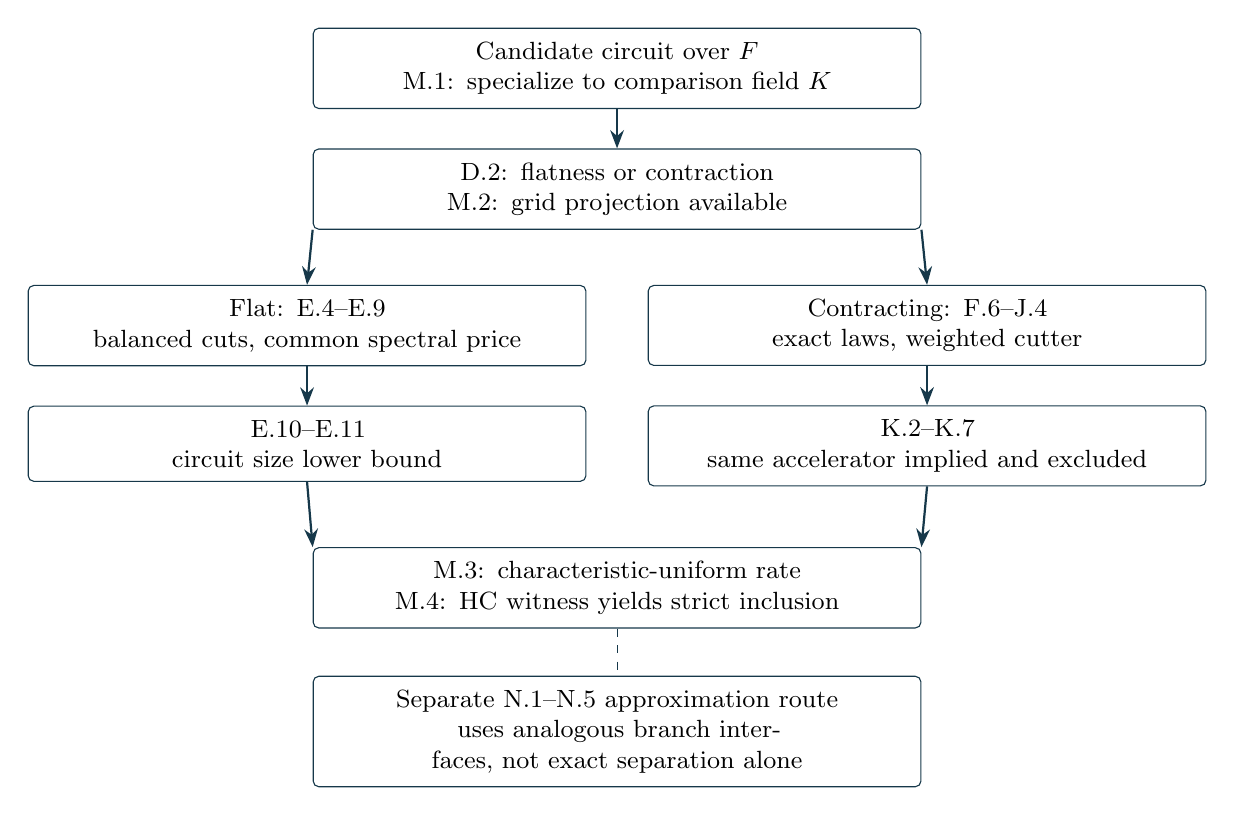
\begin{tikzpicture}[>=Stealth, font=\small,
  box/.style={draw=navy,rounded corners=2pt,align=center,text width=2.9in,inner sep=5pt},
  branch/.style={box,text width=2.65in}, line/.style={->,draw=navy,thick}]
\node[box] (m) {Candidate circuit over $F$\\M.1: specialize to comparison field $K$};
\node[box,below=5mm of m] (d) {D.2: flatness or contraction\\M.2: grid projection available};
\node[branch,below=7mm of d,xshift=-1.55in] (e) {Flat: E.4--E.9\\balanced cuts, common spectral price};
\node[branch,below=7mm of d,xshift=1.55in] (g) {Contracting: F.6--J.4\\exact laws, weighted cutter};
\node[branch,below=5mm of e] (rate) {E.10--E.11\\circuit size lower bound};
\node[branch,below=5mm of g] (acc) {K.2--K.7\\same accelerator implied and excluded};
\node[box,below=8mm of $(rate.south)!0.5!(acc.south)$] (all) {M.3: characteristic-uniform rate\\M.4: HC witness yields strict inclusion};
\node[box,below=6mm of all] (approx) {Separate N.1--N.5 approximation route\\uses analogous branch interfaces, not exact separation alone};
\draw[line] (m)--(d);\draw[line] (d.south west)--(e.north);\draw[line] (d.south east)--(g.north);
\draw[line] (e)--(rate);\draw[line] (g)--(acc);\draw[line] (rate.south)--(all.north west);\draw[line] (acc.south)--(all.north east);
\draw[dashed,draw=navy] (all)--(approx);
\end{tikzpicture}
\caption{Exact proof dependency route, with the separately justified border extension shown below. The two branches are sufficient alternatives in the same comparison field; the dashed connection denotes shared interfaces, not implication from the exact theorem.}\label{fig:dependencies}
\end{figure}

\subsection{Field transfer without losing correlations}\label{sec:field}
\begin{proposition}[Publisher M.1, same-size exact specialization]\label{prop:field}
Let $F$ and $K$ have the same characteristic, with $K$ algebraically closed. If an integer polynomial (interpreted in $F[X]$) is computed by a circuit of size $s$ over $F$, its image over $K$ admits a circuit of size $s$.
\end{proposition}
\begin{proof}
Let $k$ be the common prime field and work in the nonzero $K$-algebra $T=F\otimes_k K$. The finitely many constants of the candidate generate together with $K$ a finitely generated $K$-subalgebra $A\subseteq T$. A polynomial-ring presentation of $A$ has proper kernel. By the weak Nullstellensatz there is a $K$-algebra map $A\to K$. Lift the gate list to $A[X]$; its output identity follows from the injective map to $T[X]$. Apply the homomorphism to every gate. All references and polynomial operations survive; the target integer coefficients map to the appropriate characteristic. The gate count is unchanged.
\end{proof}
It is crucial that all constants specialize through one homomorphism. For example a root of $z^2+z+1$ in $\F_4$ cannot simply be assigned a value in $\F_2$ preserving that relation. Arbitrarily changing each occurrence would lose algebraic constraints. The algebraic closure of the prime field suffices as the fixed comparison field for each characteristic, so the cutoff need not depend on the original field. See \aud{passes/11d-field-transfer.md}{the field-transfer audit} and \pub{Paper/Transfer.lean}{21}{M.1}.

\subsection{Grid completeness: from an arbitrary target circuit to a controlled polynomial}\label{sec:grid}
Let $v:I\to V$ and $w:I\to W$ be onto incidence maps. For each incidence $i$ fix a local two-bit weight $D_i(a,b)$ in a commutative ring. The grid sum is
\[
 G(D)=\sum_{x:V\to\{0,1\}}\sum_{y:W\to\{0,1\}}
         \prod_{i\in I}D_i(x_{v(i)},y_{w(i)}).
\]
It is crucial that the same assignment to one vertex is used at all incidences. The publisher constructs HC matrices of every order $m\ge40|I|$ with value $G(D)$. The construction uses a cycle of heads, shared XOR gadgets, and incidence options: each head chooses a traversal, the two tips of each XOR gadget enforce compatible use, and each incidence contributes its selected local weight. There are at most $39|I|$ unpadded vertices; unit-weight single-option heads extend the order without multiplying the number of cycles. The permanent analogue uses factor three and requires characteristic other than two. These are projection theorems, not restrictions on candidate circuits.

The review traced the bijection between a shared assignment and a successor permutation. A fixed cycle cannot choose both inconsistent uses of a gadget; doing so would close a short cycle and omit vertices. Conversely a consistent assignment determines the local flags and the unique traversal. A finite two-incidence check with the same two shared bits gave four structural cycles, whereas sharing only one bit gave eight. A signed example gives $2+2z$ for shared choices, rather than $(3+z)^2$ under a mistaken independent-copy construction. This distinction persists under specialization to characteristic two.

For the weights used in the proof, each target variable is replaced by a one-variable affine expression or constant. An $s$-gate candidate therefore yields a grid-sum circuit with at most $5s$ gates, accounting for scalar and binary gates while retaining the original shared references. Thus if the grid sum has a large complexity, every candidate target circuit must pay it. The dimension factor $40$ (or $3$) and circuit substitution factor $5$ charge different resources. See \aud{passes/12b-hamiltonian-projection.md}{HC projection}, \aud{passes/pass13C-permanent.md}{permanent projection}, and \pub{Paper/HcGrid.lean}{18}{M.2}.

\section{Spectral prices and the geometric alternative}\label{sec:geometry}
The algebraic and metric derivations underlying this section are supplied in Appendix~\ref{sec:geometricdetail}.
\subsection{Tensor semantics and the class of prices}
For a finite party set, a tensor is a finite array indexed by one local coordinate at each party. A restriction applies a separate linear map at each party. Tensor products concatenate local coordinates; tensor sums are interpreted with compatible index sets. The binary equality wire $\langle 2\rangle_{ab}$ has entries equal to one precisely when the two endpoint coordinates agree. More generally a dimension-$r$ wire $\langle r\rangle_{ab}$ implements an $r$-valued shared index. A rank-$L$ decomposition across a bipartition can be realized by two hubs linked by one $L$-valued index, with all the outer legs carrying their respective local coordinates.

The publisher's spectral points obey nonnegativity, normalization at the scalar unit, multiplicativity for tensor product, restriction monotonicity and a cover inequality. The publisher describes this as a ``variant of Strassen's asymptotic spectrum'' \cite[p.~3]{claude}; its axioms use the upper cover inequality rather than requiring direct-sum additivity. For each such point $\varphi$ the value of an equality wire of dimension $r$ is $r^{d_\varphi(a,b)}$, defining a nonnegative pseudometric on parties. A price is a pseudometric whose restriction to any finite configuration is a limit of simultaneously scaled spectral distances $c d_\varphi$. Precise definitions and wire identities appear in Appendix A of \cite{claude} and \pub{Paper/Prices.lean}{23}{Prices.lean}. Classical spectral methods originate in Strassen \cite{strassen}; related asymptotic graph-tensor and surgery methods appear in \cite{cvz19,cz19}.

\interpret{A single spectral distance is a way to assign a consistent price to each communication wire. Unlike a single flattening, the construction may compare many positions and cuts at once. The same price must be used on all terms being compared; selecting the most convenient price separately for each summand would not give a valid inequality for their sum.}

\subsection{Why the upper-functional selection is multiplicative}\label{sec:gauges}
Proposition A.5 selects one spectral point below an upper functional $p_0$, preserving every comparison $p_0(tx)\le c\,p_0(ty)$ for \emph{all} tensor multipliers $t$. The review reconstructs why this is possible. Consider upper functionals below $p_0$ retaining the designated comparisons. A descending chain has an admissible pointwise infimum: each finite inequality can be tested at a common chain member approaching the finitely many relevant infima. By Zorn's lemma there is a minimal element $p$.

The first operation is power regularization,
\[
 r(t)=\inf_{n\ge1} p(t^n)^{1/n}.
\]
When a tensor has a finite cover, taking powers expands it by words in the cover elements. Group by multiplicities; commutativity permits the multiplicative constants in the exponential upper bounds of the finitely many cover generators to be paid once per generator. Taking roots recovers the cover inequality for $r$. Applying the multiplier comparison repeatedly preserves it after regularization. Minimality implies $r=p$ and hence $p(t^n)=p(t)^n$.

For $p(f)>0$, localize
\[
 q_f(t)=\inf_{n\ge0}\frac{p(tf^n)}{p(f)^n}.
\]
The unit is preserved by power equality. The same cover and multiplier constraints are inherited, and $q_f\le p$; hence $q_f=p$. Shifting the index of the infimum by one yields $p(t)p(f)\le p(tf)$, the reverse of submultiplicativity. A zero factor follows directly from the nonnegative upper bound. This gives multiplicativity of the selected functional. Notice that the existence of the minimal functional and the power-cover proof are substantive hypotheses of this selection argument.
\begin{counterexample}[Why the comparison must be contextual]
On the additive monoid $\N^2$ let $p(a,b)=\max(2^a,2^b)$ and take a cover to contain the element being covered. Then $p(1,0)=p(0,1)=2$, but translating by $(1,0)$ gives $p(2,0)=4$ and $p(1,1)=2$. Equality at the unit is not equality under all multipliers.
\end{counterexample}
See \aud{passes/11b-spectral-selection.md}{A.5 reconstruction}, \pub{Paper/Gauges.lean}{392}{A.5}, and the publisher's duality A.6. The selection is classical and existential; no efficient procedure for producing the point is asserted.

\subsection{One witness preserving all old wires}\label{sec:extension}
Given old parties $I$, an inclusion $\iota:I\to I'$, retractions $\pi_j:I'\to I$ and nonnegative weights $\theta_j$ summing to one, Proposition A.7 gives an enlarged spectral point dominated by
\[
 f(t)=\prod_j\varphi(\pi_j t)^{\theta_j}
\]
while preserving the value of a designated old tensor $C$. The proof constructs a gauge from the infimum of sums of $f$ over covers. Because every retraction is the identity on old parties, the gauge agrees with $\varphi$ on old tensors. Localizing at $\iota C$ and applying A.5 produces a spectral point that preserves $C$ exactly (the zero-valued case follows from domination). The designated tensor must be chosen before the point.

A.8 chooses $C$ as the product of dimension-two wires for \emph{all} ordered old pairs. The domination bounds each old distance from above. Multiplicativity and exact equality on $C$ give
\[
 \sum_{u,v\in I}\bigl(d_\varphi(u,v)-d_{\varphi'}(\iota u,\iota v)\bigr)=0.
\]
All summands are nonnegative, so each old wire distance is preserved. This is a powerful use of a single aggregate equality to prove many equalities: the one-sided comparison is indispensable.
\begin{counterexample}[Preserving the wrong tensor]
On two parties matrix rank and the indicator of being nonzero are both spectral points in the stated class. The second is dominated by the first and both agree on the scalar unit. Yet they assign values two and one to the $2\times2$ identity wire. Agreement on the unit does not fix that wire.
\end{counterexample}
For finite old and new sets, A.8's randomized retractions preserve the joint placement distribution. An approximation error $\epsilon$ on all old pairs increases the new bound by at most $\sum_j\theta_j\epsilon=\epsilon$. Compactness on finite tables followed by a common cofinal limit on finite restrictions yields a price with every required bound simultaneously. It is not necessary that each finite witness be compatible before taking the common limit. Importantly the new distances need only be \emph{at most} their expected placement distances. Treating them as equal would assert more than A.8 gives.

\scope{The A.5/A.7/A.8 arguments are reconstructed from the pinned publisher sources and archived targeted builds. They require their tensor-cover axioms and classical existence steps, not just abstract distance inequalities. See \pub{Paper/Extension.lean}{166}{A.7}, \pub{Paper/Prices.lean}{160}{all-wire equality}, and \aud{report/VP_VNP_Research_Review.pdf}{Edition 12, discussion of price extension}.}

\subsection{Crossing tensors and curvature}\label{sec:curvature}
The other geometric input is a crossing identity: a product of two equality wires can be expanded as a sum of integral coefficient tensors, each admitting two different cut decompositions. Let the wire alphabets have energies $e_1,e_2$, and write $\Theta=2(e_1+e_2)$. The review records the B.2 bounds $(N+1)P(N)$ and $(\Theta-N+1)P(\Theta-N)$ for the two product counts of the same coefficient $\Psi_N$. Here $P(M)$ counts Frobenius symbols with energy at most $M$. The underlying determinant expansion is integral; reflecting the formal variable exchanges the complementary degrees and the two cuts. The same coefficient may vanish after specialization into a small-characteristic field.

For clarity, the normalization in B.1 can be understood via partitions. Interleaving $k$ equal-size pairs of subsets into complementary residue classes gives $P(k^2E)\ge P(E)^k$. A product bound gives $\log P(E)=O(\sqrt E)$. By interleaving a nearly maximizing finite energy into increasingly large energies, the ratio $\log P(E)/\sqrt E$ converges to its finite positive supremum $\kappa$. The review's separate partition-series derivation identifies $\kappa=\pi/\sqrt3$ for natural logarithms: the series $Z(t)=\prod_{j\ge1}(1-e^{-2tj})^{-1}$ satisfies $t\log Z(t)\to\pi^2/12$, whereas optimizing the growth envelope gives $\kappa^2/4$. The numerical value is not needed by B.3. The necessary point is uniform control at the coefficient index selected by the spectral evaluation.

Select one maximizing coefficient $\Psi_N$ for a fixed spectral point. Use its two decompositions, not two separately maximizing coefficients. With energy budgets approximately $p^2 n,q^2 n$, the two associated normalized hub weights satisfy
\[
 r^2=\frac{\Theta-N}{n},\qquad (r')^2=\frac{N}{n},\qquad
 r^2+(r')^2\le2(p^2+q^2).
\]
Both inequalities survive the limit for this common choice. This is the joint comparison B.3 that C.2 consumes. A Manhattan-square test in the audit shows why using separate choices would be invalid: the two hub bounds require $r,r'\ge2$ while the joint squared budget is only four. Separately choosing $(2,0)$ and $(0,2)$ hides the contradiction. The complete determinant and minor-sign checks are in \aud{passes/11a-crossing.md}{Pass 11A} and \aud{report/VP_VNP_Research_Review.pdf}{the B.1/B.2 derivation}; the formal identity is \pub{Paper/Identity.lean}{699}{B.2}.

The endpoint curvature inequality C.1 is central. Suppose $w(x,v)=2D$ and $w(x,m),w(v,m)\le D$; the triangle inequality forces equality for the two legs. For $b=w(z,m)$ define
\[
 \Gamma=b^2-\frac12\bigl(w(z,x)^2+w(z,v)^2\bigr).
\]
The desired bound is $\Gamma\le-D^2$. We state the key reduction to make the order of limits explicit. At fixed $T\ge2$, set $\theta=1/T$, form the extended fan through A.8 and the averaged stable seminorm $N(\cdot)$ obtained from a translation-invariant limiting mean of squared distances. Write $\Lambda_2\le(D+b)^2$ for the average squared spoke length. The publisher's four fan estimates, audited in Pass 9, are
\begin{align*}
 N(1,0)&\ge D, &N(1,-1)^2&\le D^2(1-\theta+\theta^2),\\
 N(0,1)^2&\le\theta^2\Lambda_2,\\
 N(1,-1-A)^2&\ge A^2\theta^2\Lambda_2+A\theta\Gamma-4A\theta^2D(D+b)
 \qquad (A\ge1).
\end{align*}
Here the same fan mean and $\Lambda_2$ must apply to all $A$ at fixed $T$. C.2 gives a second-difference identity for $f(j)=N(1,-1-j)^2$. Subtracting $j^2\theta^2\Lambda_2$ leaves a discretely concave function $\psi$, so
\[
 \psi(A)\le\psi(0)+A(\psi(0)-\psi(-1)).
\]
Set $p=N(1,0)^2$, $q=N(1,-1)^2$ and $\beta=\theta^2\Lambda_2$.
Since $\psi(-1)=p-\beta$, the slope bound gives
$A[\theta\Gamma-4\theta^2D(D+b)-(q-p+\beta)]\le q$.
Divide by $A\theta$ once. The upper bound on $q-p$ and
$\Lambda_2\le(D+b)^2$ give a finite remainder
\[
 \Gamma+D^2 \le \frac{qT}{A}+\frac{6D^2+6Db+b^2}{T}.
\]
At fixed $T$ the same $q$ serves every $A$. Letting $A\to\infty$ gives
\[
 \Gamma+D^2\le \frac{6D^2+6Db+b^2}{T}.
\]
Finally send $T\to\infty$. The right-hand numerator depends only on the original points. This yields
\begin{equation}\label{eq:cat}
 w(z,m)^2\le \tfrac12 w(z,x)^2+\tfrac12 w(z,v)^2-\tfrac14 w(x,v)^2.
\end{equation}
Independently of the fan chosen for $T$, $0\le q\le D^2$. Thus $A=T^2$ also sends both terms of the finite remainder to zero. The choice $A=T$ leaves the intercept term equal to $q$ and supplies no uniform decay from these estimates. The successive limits above are sufficient. For a metric square with distances along its edges, two opposite corners $x,v$ are distance two; taking the other corners $m,z$ gives $w(z,m)^2=4$ but the right side of \eqref{eq:cat} is zero. The price hypothesis is therefore substantive; not every pseudometric is a price.

\scope{The four fan estimates and C.2 are inputs to this derivation. For this revision a separate exact-rational check exercised the finite remainder on 5,664 scalar configurations, including 480 with $D=0$. The cases test the displayed algebra. Realizing a given scalar configuration by a geometric fan is a separate question. The archived 44-module targeted build for C.1 and subsequent C.3/D.2 replay concern the exact publisher statements. See \pub{Paper/Fan.lean}{987}{C.1 endpoint}, \pub{Paper/Means.lean}{465}{C.2}, and \aud{checks/pass09_endpoint_replay_results.json}{the focused receipt}.}

\subsection{D.2: why lack of contraction produces Euclidean prices}\label{sec:d2}
Fix a field $K$. For a price on $\operatorname{Mat}_\mu(\F_2)$ define $D(r)$ as the root-mean-square distance between $a$ and $a+W$ under uniform $a$ and a uniform rank-$r$ matrix $W$. The binary field here indexes configurations, and need not be the field over which the circuit is computed. The publisher's Definition D.1 states:
\begin{itemize}[leftmargin=1.5em,itemsep=1pt]
\item Flatness: all finite subsets of all Euclidean spaces with their metrics are $K$-prices.
\item Contraction: some $\mu\ge2$ and $1\le s<\sqrt\mu$ satisfy $D(\mu)\le sD(1)$ for every such $K$-price.
\end{itemize}
D.2 asserts that at least one holds. We explain the structure of its proof. C.3 realizes each price as the pullback of a complete CAT(0) price space. For uniform transversal rank-$i$ and rank-$j$ increments, the CAT(0) quadrilateral inequality averaged over $a$ implies
\[
 D(i+j)^2\le D(i)^2+D(j)^2 \quad (i+j\le\mu).
\]
If contraction fails, take prices with $D(1)=1$ and $D(\mu)$ tending to $\sqrt\mu$. The finite normalized configurations are bounded and admit a limit price. Subadditivity gives $D(r)^2\le r$. Equality at $\mu$ and the inequality at $(r,\mu-r)$ force $D(r)^2=r$ for all ranks. At this limit every quadrilateral defect in the finite average is nonnegative and their average is zero; hence each defect is zero.

The remaining rigidity argument in D.2 upgrades equality of averages to equality of every squared distance. With $n_a(W)=w(a,a+W)^2$ and for transversal increments define
\[
 B_a(W,W')=\tfrac12[n_a(W+W')-n_a(W)-n_a(W')].
\]
The quadrilateral equalities yield base-point invariance along transversal shifts and additivity of $B_a$ on transversal triples. Elementary rank-one exchanges over $\F_2$ imply that $B_a$ takes one value $\lambda(a)$ on transversal rank-one pairs. The translation identity gives a sign reversal of $\lambda$ along a rank-one step. A rank-two step both reverses it (by the rank-two identity) and preserves it (as two rank-one steps), forcing $\lambda=0$. Additivity on transversal sums and rank-one normalization yield $w(a,a')^2=\operatorname{rank}(a-a')$. The binary diagonal matrices therefore form the vertices of an isometric Euclidean cube. C.4(f) fills the cube by geodesic interpolation, one coordinate at a time. Arbitrarily large cubes yield every finite Euclidean configuration after translation and scaling.

\interpret{The alternative is a rigidity-versus-saving dichotomy. If a strict uniform saving cannot be extracted, normalized price inequalities become tight; equality rigidifies a finite geometry enough to supply Euclidean configurations. If the saving exists, the contracting branch uses it to reduce network loads. This need not be a mutually exclusive dichotomy and the proof does not compute the case.}
\scope{D.2 is a pinned stated result. Our exposition traces its hypotheses and the equality mechanism; the full geometric construction remains in the source and its formal dependencies. See \pub{Paper/Alternative.lean}{43}{definition}, \aud{passes/07-field-alternative.md}{field alternative audit}, and \aud{passes/08-price-space-completion.md}{price-space completion}.}

\section{The flat branch: from an arbitrary circuit to a common price}\label{sec:flat}
\subsection{The auxiliary polynomial and its coefficient tensor}
Fix $k\ge2$ and $\ell\ge100\sqrt{k}$. Put $N=\binom{k}{2}$ and assign an $\ell$-bit string to each edge of the complete graph on $k$ vertices. At vertex $a$, let $X_{a,x_a}$ be the variable indexed by the tuple of strings on its incident edges. The polynomial $f_{k,\ell}$ sums the product of the $k$ chosen variables over all shared edge assignments. Its multidegree is one in each of the $k$ blocks. The coefficient tensor $t$ has one equality constraint for each pair of edge endpoints; it is the tensor product of $N$ dimension-$2^\ell$ wires. A circuit computing this polynomial need not use those edges in any recognizable way.

The key reduction is to recover a useful tensor representation from the output coefficients of any circuit. Fix a finite index set $T$ for each block (padding where necessary), and an arbitrary gate list $(p_i)_{i<L}$. For $S\subseteq[k]$ and a block assignment $x$, let
\[
 m_S(x)=\prod_{a\in S}X_{a,x_a},\qquad c_{i,S}(x)=[m_S(x)]p_i.
\]
The bracket is the exact monomial coefficient, with no contributions from unselected blocks. At a product $p_i=p_u p_v$ the identity
\begin{equation}\label{eq:split}
 c_{i,S}=\sum_{B\subseteq S}c_{u,B}c_{v,S\setminus B}
\end{equation}
holds because each variable with exponent one is assigned to exactly one of the ordered input sockets. The identity permits repeated predecessor indices $u=v$, high intermediate degree and cancellation. A sum gate adds its two coefficient tables.

\begin{proposition}[Balanced-cofactor decomposition, publisher E.4; review reconstruction]\label{prop:balanced}
Let $k\le3|A|\le2k$ define a balanced subset. For any $L$-gate list and every large $S$ (meaning $3|S|>2k$), there exist complementary coefficient tables $H^{i,S}_{\delta,A}$ depending only on the coordinates in $S\setminus A$ such that
\begin{equation}\label{eq:cofactor}
 c_{i,S}(x)=\sum_{\substack{A\subseteq S\\k\le3|A|\le2k}}\sum_{\delta<L}
 c_{\delta,A}(x)H^{i,S}_{\delta,A}(x|_{S\setminus A}).
\end{equation}
In particular the full block component is a sum over balanced cuts, with at most $L$ separated products for each fixed cut.
\end{proposition}
\begin{proof}
Induct strongly on the original gate index, retaining the same $k$ throughout. For a scalar or variable, a large set $S$ has at least two blocks and its coefficient is zero. At addition combine the two earlier collections entrywise. For each ordered allocation $B\sqcup C=S$ in \eqref{eq:split}, choose the left component if $3|B|\ge k$, and the right component otherwise. In the latter case $3|C|>k$. Denote the chosen set by $D$, its earlier gate by $r$, and the sibling gate by $s$. If $3|D|\le2k$, the chosen component is balanced; enter $c_{s,S\setminus D}$ as the complementary factor at $(r,D)$. If it is larger, apply the induction hypothesis to $(r,D)$ and multiply each resulting cofactor by the sibling coefficient. It depends only on $(D\setminus A)\sqcup(S\setminus D)=S\setminus A$. Summation of all ordered splits adds entries belonging to the same original gate and balanced subset. The induction descends in gate index even when $D=S$ and the sibling is a constant. This avoids a non-decreasing recursion in subset size. Setting $S=[k]$ at the output gives the claimed separated coefficient tables. Packaging each table as a polynomial on its own block set preserves the coefficient identity because the sets are disjoint.
\end{proof}
\begin{example}[One gate, two contexts]
For four blocks write $g=A_0B_0$ once and form $gC_0D_0+gC_1D_1$. Across the cut $\{A,B\}\mid\{C,D\}$ the cofactor at $g$ is $C_0D_0+C_1D_1$. It carries both contexts without introducing a second label for $g$. Keeping only the first use loses the coefficient of $A_0B_0C_1D_1$. If a repeated input is added twice it can cancel in characteristic two; the coefficient recurrence still holds.
\end{example}
This proof bounds the number of products for a fixed cut, not the circuit complexity of computing each cofactor. That distinction is exactly what allows it to treat arbitrary circuits without a formula-size expansion. The original source is \pub{Paper/Flat.lean}{229}{E.4}; the review's detailed proof is \aud{passes/pass13A-gate-reuse.md}{Pass 13A}. The formal lemma also admits commutative semirings at this stage.

\subsection{Routing a cut through hubs and paying for a common selector}\label{sec:selector}
For each balanced set $A$, route the separated coefficient sum through two hubs, one for each side, with an internal wire of dimension $L$ carrying the original gate index. Each outer end connects to its own hub by a dimension-$2^\ell$ wire. Let $T_A$ denote this hub tensor. By the coefficient decomposition and A.3, $t$ is a sum of restrictions of $T_A$. There are $J\le2^k$ candidate sets; different summands can correspond to different cuts.

Let $P$ be the set of parties with nontrivial output coordinates. Write $g_\varphi(P)$ for the exponent of the shared size-two diagonal selector on $P$, so a diagonal selector of size $r$ has spectral value $r^{g_\varphi(P)}$. We reproduce the key E.7 estimate under its exact restriction hypotheses:
\begin{proposition}[Mixed-cut spectral bound, publisher E.7]\label{prop:mixed}
If $t$ is the sum of restrictions of $T_1,\ldots,T_J$ and the output is trivial outside $P$, then for any spectral point $\varphi$,
\begin{equation}\label{eq:mixed}
 \varphi(t)\le J^{g_\varphi(P)}\max_{1\le j\le J}\varphi(T_j).
\end{equation}
\end{proposition}
\begin{proof}[Reconstruction of the exact case]
Take the $n$-fold tensor power, expand by words in $[J]^n$, and group by the vector of multiplicities of each letter. There are at most $(n+1)^J$ types. For a type $\tau$, choose a representative word and a permutation of positions for each word of that type. One common index among the $r_\tau$ words allows every party in $P$ to permute its output positions according to the same permutation. The other parties have no nontrivial output index to move. The sum of terms of type $\tau$ is thus a restriction of the representative product together with a shared selector of size $r_\tau$. Since $r_\tau\le J^n$, multiplicativity and the cover bound give
\[
 \varphi(t)^n\le(n+1)^J\bigl[J^{g_\varphi(P)}\max_j\varphi(T_j)\bigr]^n.
\]
If the exponential base is zero the desired claim follows at once. Otherwise take $n$th roots and send $n\to\infty$ with $J$ and all tensors fixed. The polynomial overhead has root tending to one. This proves \eqref{eq:mixed}.
\end{proof}
The approximate variant N.3 additionally extracts a Laurent coefficient; a polynomial-in-$n$ factor is charged at fixed degree envelope and fixed number of parties. It disappears in the same order of limits. One cannot let $J$ grow with $n$ without a new estimate: if $J=n$, the number of possible multiplicity types is at least $2^{n-1}$. Nor can one charge a selector on a party outside the actual output support. For example $E_{00}+E_{11}$ has matrix rank two whereas each term has rank one; a selector visible to only one of the output parties cannot coordinate both indices.

\begin{counterexample}[Exchanging the witness and cut quantifiers]\label{ex:mixed}
The common price is also necessary before maximizing over cuts. Consider two candidate wire tensors, with two flattening-rank tests assigning $(2,1)$ and $(1,2)$. The minimum of the row maxima is two; the maximum of the column minima is one. Choosing a favorable functional separately for each term would silently exchange the quantifiers. The review records the 84 signed tensor-power entries and 1,428 balanced directions checked in the Pass 14A finite controls; the general mixed-cut bound rests on the proof above. See \aud{passes/14a-flat.md}{Pass 14A}, \pub{Paper/Convex.lean}{22}{E.7}, and \pub{Nc/Price/BorderFew.lean}{134}{the type-count estimate}.
\end{counterexample}


\subsection{One common Euclidean witness and the price of the end selector}\label{sec:euclid}
In the flat case any finite Euclidean configuration is a price. This does not permit freely replacing every distance by Euclidean length in a tensor inequality: a common spectral point and one scale have to approximate \emph{all} distances simultaneously. E.8 and E.9 establish the additional selector estimate needed to pay for the mixed-cut sum.

Here is the quantitative mechanism. If $m_i$ is the midpoint of $a_i,b_i$ in a finite Euclidean configuration, choose a shared fair placement between the two maps. The extension argument of Section~\ref{sec:extension} preserves the product of all old wires and one designated old diagonal tensor. Positivity and one-sided domination force each factor, and then every old wire, to retain its value. The new labels become exact midpoints in the extended price. Suppose the original scaled spectral distances approximate the Euclidean distances to $d\le1$. With $R$ the sum of pair distances and $q$ the number of labels, the midpoint inequality bounds the displacement from the old Euclidean midpoint to the new label. Moving the $q$ selector legs one at a time gives error at most
\[
 q\sqrt{d(2R+4)}.
\]
Thus for per-level allowance $\eta$ one may choose
\[
 d=\min\left(1,\frac{\eta^2}{(q^2+1)(2R+4)}\right).
\]
Crucially this tolerance is selected before the spectral witness and applies to every needed triple of maps. The internal extensions may differ, but the inequality obtained is for the same original witness.

At each end position $\pm e_i/2$ of a $k$-cube, start with the random sign map $s e_i/2\mapsto s\chi_i\chi/2$ where $\chi\in\{-1,1\}^k$. Each such map has image in two positions on a diagonal of length $\sqrt k$. Averaging the first $j$ independent signs gives maps into the ternary half-cube. Each next level is a pointwise midpoint of two preceding maps. Include all those points and every possible hub position in the configuration before choosing the spectral point. The average satisfies $\mathbb E[\chi_i\chi_j]=\delta_{ij}$, so after $k$ levels it recovers the end positions. Taking $\eta=\Delta/(2k)$ and initial pair error at most $\Delta/2$ gives a selector exponent $G$ with scaled bound
\begin{equation}\label{eq:selector}
 cG\le \sqrt k+\Delta.
\end{equation}
The accumulated loss is per depth, not per leaf of the binary averaging tree. Coincident logical end positions do not create extra geometric cost; the pullback preserves the image exponent. See \pub{Paper/Convex.lean}{318}{cube induction} and \aud{passes/14a-flat.md}{E.8--E.9 reconstruction}.

\subsection{Paying-cut geometry and the scalar inequality}\label{sec:paying}
Place the two ends of an edge $a<b$ at $+e_a/2$ and $-e_a/2$, with signs assigned according to the cut in the routed tensor. The original wire length is one. For a balanced cut $A$, define $s_a=+1$ for $a\in A$ and $-1$ otherwise, and
\[
 u_A=\sum_{a<b\text{ crossing }A}s_a e_a,\qquad
 \gamma=\frac{2}{9\sqrt k},\qquad x_A=\gamma\frac{u_A}{\|u_A\|}.
\]
Since $\langle u_A,s\rangle=|A|(k-|A|)\ge2k^2/9$, Cauchy--Schwarz gives $\|u_A\|\ge2k\sqrt k/9$. Place the two hubs at $\pm x_A$. For unit $e$ use
\[
 \|e/2-x\|\le\tfrac12+\|x\|^2-\langle e,x\rangle,
\]
which follows from the tangent inequality for the square root at $1/4$. Summing the end lengths yields at most
\[
 N+2N\gamma^2-2\gamma\|u_A\|\le N-4k/81,
\]
where $N=k(k-1)/2$. The middle length is $2\gamma$. Both hubs for \emph{every} balanced set are included before choosing the common witness. Now apply Proposition~\ref{prop:mixed} and choose the paying cut for that witness.

Figure~\ref{fig:flat-routing} illustrates the distinction between the original and routed tensor.
\begin{figure}[!htbp]
\centering
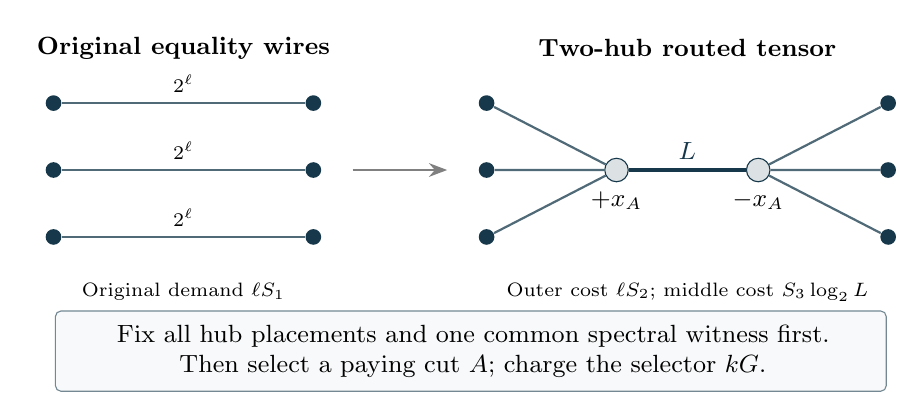
\begin{tikzpicture}[font=\small,>=Stealth, endpt/.style={circle,fill=navy,inner sep=2pt}, hub/.style={circle,draw=navy,fill=navy!15,inner sep=3pt}, wire/.style={draw=navy!75,thick}]
\node[font=\small\bfseries] at (1.65,2.6) {Original equality wires};
\node[font=\small\bfseries] at (8.05,2.6) {Two-hub routed tensor};
\foreach \i in {0,1,2}{
 \pgfmathsetmacro{\yy}{1.9-.85*\i}
 \node[endpt] (a\i) at (0,\yy) {};
 \node[endpt] (b\i) at (3.3,\yy) {};
 \draw[wire] (a\i)--node[above, font=\scriptsize] {$2^\ell$}(b\i);
 \node[endpt] (c\i) at (5.5,\yy) {};
 \node[endpt] (d\i) at (10.6,\yy) {};
}
\node[hub,label=below:{$+x_A$}] (hp) at (7.15,1.05) {};
\node[hub,label=below:{$-x_A$}] (hm) at (8.95,1.05) {};
\foreach \i in {0,1,2}{\draw[wire] (c\i)--(hp);\draw[wire] (hm)--(d\i);}
\draw[navy,very thick] (hp)--node[above] {$L$}(hm);
\draw[->,gray,thick] (3.8,1.05)--(5.0,1.05);
\node[font=\scriptsize,align=center] at (1.65,-.5) {Original demand $\ell S_1$};
\node[font=\scriptsize,align=center] at (8.05,-.5) {Outer cost $\ell S_2$; middle cost $S_3\log_2 L$};
\node[draw=navy!60,fill=navy!3,rounded corners=2pt,align=center,text width=10.2cm,inner sep=5pt] at (5.3,-1.25) {Fix all hub placements and one common spectral witness first.\par Then select a paying cut $A$; charge the selector $kG$.};
\end{tikzpicture}
\caption{Flat-branch routing, schematically showing three crossing equality wires of a single candidate cut. The full coefficient tensor has all $N$ wires, including edges on the same side; the drawing is not a Euclidean embedding of the complete instance. The comparison uses one witness for all candidate cuts before any paying cut is selected. See Eq.~\eqref{eq:budget}.}\label{fig:flat-routing}
\end{figure}

Let $S_1,S_2,S_3$ be the sums of original, outer and middle-wire exponents (the last a single wire), respectively, and let $G$ be the logical end selector exponent. Taking base-two logarithms of \eqref{eq:mixed}, and using $J\le2^k$, gives
\begin{equation}\label{eq:budget}
 \ell S_1\le kG+\ell S_2+S_3\log_2L.
\end{equation}
At $\Delta=1/(1000k)$ the common witness and its scale $c$ obey
\begin{align}
 cS_1&\ge N(1-\Delta), &cS_2&\le N-4k/81+2N\Delta,\label{eq:pricebounds}\\
 cS_3&\le4/(9\sqrt k)+\Delta, &cG&\le\sqrt k+\Delta.
\end{align}
Here $c$ is a metric scale, not the universal lower-bound constant. The proof uses the original $S_1$ and the paying cut's $S_2,S_3$ in the \emph{same} spectral point. The total pair approximation loss in the wire difference is $3\ell N\Delta$, independent of the number of candidate cuts.

\begin{theorem}[Review strengthening of the E.10 scalar margin]\label{thm:twelve}
Under \eqref{eq:budget}--\eqref{eq:pricebounds}, $k\ge2$, $\ell\ge100\sqrt k$ and $L\ge1$,
\[
 \log_2 L>\frac{\ell k\sqrt k}{12}.
\]
\end{theorem}
\begin{proof}
Write $z=\log_2 L\ge0$. Multiply \eqref{eq:budget} by the common scale, use the four one-sided bounds, and rearrange:
\[
 (4/(9\sqrt k)+\Delta)z
 \ge \ell(4k/81-3N\Delta)-k(\sqrt k+\Delta).
\]
Since $3N\Delta\le3k/2000$, $k(\sqrt k+\Delta)\le\ell k(1/100+1/10000)$, and $(4/(9\sqrt k)+\Delta)\sqrt k\le4/9+1/1000$, multiplication by $\sqrt k$ yields
\[
 az\ge b\ell k\sqrt k,\qquad
 a=\frac{4009}{9000},\quad b=\frac{7651}{202500}.
\]
Both constants are positive and $12b-a=1073/135000>0$. Hence $b/a>1/12$ and the strict conclusion follows.
\end{proof}
The source states denominator 16, and its printed proof and Lean arithmetic already establish denominator 14. The review's denominator 12 is a modest sharpening, not a correction to the final theorem. The independently checked scalar comparison at $k=4,\ell=200,z=138$ gives positive slack $15551/162000$ when each one-sided bound is saturated, even though $z<\ell k\sqrt k/11$. Thus the scalar relaxation alone does not justify denominator 11. No synthetic price in this example is asserted to arise from a circuit. The proof of Theorem~\ref{thm:twelve} and its circuit-level bridge checked in Lean with the archived freshly built Paper.Rate object; they were not among the publisher's five public Comparator targets. See \aud{checks/pass14a_margin_results.json}{scalar receipt}, \aud{checks/pass14a_circuit_results.json}{circuit-level receipt}, and \pub{Paper/Rate.lean}{123}{publisher arithmetic}.

\subsection{Conversion to the target size}\label{sec:flatconvert}
Let a candidate circuit of size $s$ compute a grid-complete target of matrix order $m$ with projection factor $\kappa$ (40 for HC, 3 for the permanent in allowed characteristics). The grid construction gives a circuit of size at most $5s$ for $f_{k,\ell}$ whenever
\[
 \kappa k^3\ell 2^{k\ell}\le m.
\]
For all sufficiently large $m$, set $B=\lfloor\log_2m\rfloor$ and choose the largest integer $r$ satisfying $200r^3\le B$. Then $r\ge\kappa+2$ at the specified threshold in E.11, and
\[
 \log_2m< B+1\le200(r+1)^3\le1600r^3.
\]
Set $k=r^2$, $\ell=100r$. The polynomial factor $\kappa r^6(100r)$ is at most $2^{107r}$ and hence at most $2^{100r^3}$ in the range used. The grid fits. The publisher's weaker /16 bound already gives $\log_2(5s)\ge25r^4/4$ and therefore $\log_2s>r^4$. Combining the inequalities proves
\[
 \log_2s>\frac{(\log_2m)^{4/3}}{1600^2}.
\]
This calculation applies to every sufficiently large $m$, not just selected cube sizes. It finishes the flat-case exclusion under the same comparison field. See \pub{Paper/Rate.lean}{337}{E.11}, \aud{passes/14a-flat.md}{rate conversion}.

\section{The contracting branch: from a geometric saving to exact weighted cuts}\label{sec:contract}
Appendix~\ref{sec:contractdetail} supplies the window estimates and related implementation details.
The second branch does not start with a low-rank decomposition of the target. Instead, the contraction condition supplies reusable tensor identities with a bound on the amount of data crossing a boundary. These identities are then composed into a tree-shaped computational interface. The point is not that the original arbitrary circuit was a tree; it is that the weighted computation derived from it can be cut under explicit resource bounds.

\subsection{Uniform quadratic inequality before choosing the group}\label{sec:groups}
Let $U_h$ be the upper unitriangular group over $\F_2$, with $b=2^{h(h-1)/2}$ elements and generators $x_j=1+E_{j,j+1}$. Conditional on the contracting data, the publisher's F.6 gives a uniform price inequality on the Cayley graph for $h=lu$, $l\ge2$, where $u$ and $C_{\rm P}$ depend only on the contracting parameters:
\[
 b^{-2}\sum_{g,k\in U_h}w(k,gk)^2
 \le C_{\rm P}\sum_{j<h-1}b^{-1}\sum_{k\in U_h}w(k,x_jk)^2.
\]
The review reconstructed the final averaging estimate from the preceding window inequality and near-orthogonality assumptions in F.2--F.5. To clarify why the constant is uniform, realize the price in a complete CAT(0) space, and project a map $z$ to the fixed-point sets $P_i$ for the window generators. With $k_0$ windows, let $\Phi(z)=\sum_i d(z,P_i z)^2$. Under the stated contraction/angle hypotheses, the averaging step satisfies
\[
 \Phi(z')\le(1-\delta/k_0)\Phi(z),\qquad
 k_0 d(z,z')^2\le\Phi(z)-\Phi(z'),\qquad \delta=1/2.
\]
If $\Delta_\Phi=\Phi(z)-\Phi(z')>0$, then
\[
 d(z,z')\le\sqrt{\Delta_\Phi/k_0}
 \le\frac{\Delta_\Phi}{\sqrt{\delta\Phi(z)}}
 \le\frac{2}{\sqrt\delta}(\sqrt{\Phi(z)}-\sqrt{\Phi(z')}).
\]
The same is trivial at zero. Iterating telescopes the path length, even though the rate factor approaches one as the window count increases. Completeness gives a common fixed point. Each generator occurs in at most two windows; the finite-window estimate supplies a constant $C_{\rm P}$ independent of $h$. This is the important order of choices, not a proof that every metric has this inequality. The earlier window and angle results are publisher premises here. See \pub{Paper/Groups.lean}{1085}{F.6} and \aud{passes/pass13B-gain.md}{the uniformity audit}.

For unordered vertex pairs $\mathcal P$ and graph edges $\mathcal E$ put $\alpha=2/[b(b-1)]$ and $\beta=2/b$. The finite-population conversion gives
\begin{equation}\label{eq:poinc}
 \sum_{e\in\mathcal P}\alpha w_e^2\le C'_0\sum_{\nu\in\mathcal E}\beta w_\nu^2,
\end{equation}
where one may take integer $C'_0\ge2C_{\rm P}+1$. Fix $C_1=4C'_0$, then choose a multiple $h$ of $u$ satisfying $h\ge\max(3,2u,4(1+8C_1))$. The later stage inequality needs $1+8C_1\le h/4$. If $C_1$ depended on $h$ in an uncontrolled way this choice might be circular.

\subsection{From the dual inequality to a menu of exact local laws}\label{sec:laws}
Define the weighted dual norms $\|n\|_{\mathcal P}^2=\sum n_e^2/\alpha$ and $\|y\|_*^2=\sum y_\nu^2/\beta$. Let $Z_1,Z_2$ be the norms of the all-ones vectors in these spaces and $c_0=\sqrt{C'_0}$. Choose an integer $a\ge4(Z_1+Z_2)+1$. Rounding a nonnegative unit-ball load up gives $\sigma=\lceil ax\rceil$ with $\|\sigma\|_{\mathcal P}\le R=a+Z_1$. For any price put $W^2=\sum_{\nu}\beta w_\nu^2$. Cauchy--Schwarz and \eqref{eq:poinc} yield
\[
 \langle\sigma,w\rangle\le c_0RW.
\]
For $W>0$, the vector $y_\nu=c_0R\beta w_\nu/W$ has norm $c_0R$ and attains the right side; its ceiling $B$ still dominates the old charge and has norm at most $c_0R+Z_2$. If $W=0$, zero load suffices. The resulting integral ball is finite. The entire menu is fixed independently of the price, although a maximizing member depends on it.

\begin{example}[A menu is not one universal choice]
For nonnegative $w=(w_1,w_2)$, $w_1+w_2\le2\max(w_1,w_2)$. The menu $\{(2,0),(0,2)\}$ dominates the old load $(1,1)$ in this support-function sense. Neither fixed member dominates it for both coordinate vectors. An existential choice depending on a price cannot be moved outside that price's universal quantifier.
\end{example}
For integral loads $D$, let $W^D$ denote the product of $D_e$ dimension-two equality wires. Multiplicativity gives $\log_2\varphi(W^D)=\langle D,d_\varphi\rangle$. Thus the price inequality has the form $\forall\varphi\,\exists B\in\mathcal B:\varphi(W^\sigma)\le\varphi(W^B)$. By A.6 it yields exact tensor covers of sufficiently large powers with a subexponential number of summands; in each summand the local tensor restrictions act on wires from the finite menu. The duality step uses nonvanishing at the all-zero assignment and a normalized upper functional. The certificate argument fixes the set of cover generators before raising powers; repeated substitutions exchange copies of the original tensor, and the sum of the certificate weights bounds the number of final branches. The resulting cover is a literal weighted tensor identity rather than an approximate probabilistic routing rule.

This is the bridge from spectral inequalities to a finite set of exact local laws over a finitely generated coefficient subring $A$. The bounds on channel loads include upward rounding, a common code index, and the coefficient weights. G.2 chooses the law family once the geometry is fixed; it is not chosen separately for each input circuit. The full G.2 construction and F.6 hypothesis are essential. See \pub{Paper/Gauges.lean}{560}{A.6}, \pub{Paper/Laws.lean}{425}{G.2} and \aud{passes/pass13B-gain.md}{dual norm and rounding reconstruction}.

\subsection{Tower routing, host multiplicity, and the load invariant}\label{sec:tower}
The tower in H.1 is built using reductions of $\operatorname{SL}_h$ over the truncated binary polynomial ring. At one layer the reduction kernel is described by trace-zero leading coefficients; chains of index-two subgroups give successive chamber projections of fibre $b$. The deleted-generator subgroups act freely in their relevant orbits, and projection restricts to a bijection on those orbits. Host bijections assign exactly $b$ children to a host. The same map must be used in the routing and in the multiplicity bound. Arbitrarily choosing hosts can overload a chamber.

For initial routing, the diameter estimate in the formal H.1(d) statement is $O_h((n+1)^7)$. Two translated word routes through an intermediate chamber give a congestion bound of $4m(N+X^2)$ for word-length bound $m$ and initial chamber count $X$. The printed argument explicitly gives the stronger cubic diameter; it is reconstructed in Section~\ref{sec:cubic}. Both exponents produce the polylogarithmic overhead needed here.

Write $v_j$ for the number of chambers at a stage, $Q_j$ for the quadratic load, and $d=\sqrt{C_1}a_1/b$ for the padding allowance. At the next stage $v_{j+1}=v_j/b$. Under the G.2 gain and routing multiplicity bounds H.2 gives
\begin{align}
 Q_{j+1}&\le \frac{\sqrt{1+8C_1}}{\sqrt h}Q_j+d v_{j+1}\le\tfrac12Q_j+d v_{j+1},\\
 Q_{j+1}+dv_{j+1}&\le\tfrac12(Q_j+dv_j)\quad(b\ge4).\label{eq:load}
\end{align}
The second line follows since $2/b\le1/2$. The additive rounding cost is absorbed by augmenting the potential before iterating. Cauchy--Schwarz converts the quadratic norm to a bound on the incident load at a node. With logarithmic depth, the publisher's bounds are of form $\Lambda M^{1-\gamma}(N+M^2)$ locally and $\Lambda M(N+M^2)$ globally, where $\gamma=1/\log_2b>0$ and $\Lambda$ is a polylogarithmic factor depending on the fixed parameters. The exceptional terminal packet IDs are charged separately. The H.2(d,e) structure and all-copy bounds also count consumed and padded variables, not just live edges.

The independent routing control explicitly enumerated $\operatorname{SL}_3(\F_2[s]/(s^2))$ (43,008 elements), successive chamber counts 5,376 and 672, and 72,576 selected routes. The observed middle multiplicity was eight and outer multiplicity at most two; the adversarial host collapse produced 64 children instead of eight. This small instance does not satisfy the large-$h$ gain hypothesis. It checks the routing mechanism, not the existence of the G.2 law family. See \aud{passes/14b-tower.md}{H.1--H.2 audit} and \pub{Nc/Tow/Load.lean}{364}{quadratic estimate}.

\subsection{Preservation of the weighted global value}\label{sec:glue}
Let each node $p$ contribute a local function $\phi_p$ of incident packet values in a commutative ring. A wire has one variable shared by its holders. The total value is the finite sum of products of the local functions. A local law is used in each layer of a move; distributivity expands the old agreement condition into a weighted sum of admissible replacements. Channel words contain a law index and its payload. A self-delimiting encoding, plus connectedness of the channel graph, ensures that the same sequence of indices is used by all incident roles. The outcome records lengths; those lengths alone do not identify the index sequence. A final marker and padding produce the final packet even at zero layers. Some bounded good outcomes are unrealizable and contribute zero. The source uses the whole sum, not the value of each outcome separately.

\begin{proposition}[Shared-boundary identity; local regrouping]\label{prop:glue}
Fix a feasible collection of shared variables and a partition of the network nodes into pieces. Let $B$ be the set of distinct current packet IDs crossing between pieces. For a boundary assignment $b$ define $V_j(b)$ as the sum of the product of local factors of piece $j$ over internal assignments consistent with $b$. Then the total value of the fixed network is
\begin{equation}\label{eq:glue}
 Z=\sum_{b\text{ on }B}\prod_j V_j(b).
\end{equation}
\end{proposition}
\begin{proof}
Restriction of a global assignment gives a unique common boundary word and one internal assignment for each piece. Conversely assignments of the pieces consistent with that word determine a unique global assignment; every packet is assigned at its holders by the same ID. The maps are inverse, and each node factor occurs exactly once. Regroup the finite sum by the word and apply distributivity. No positivity, division, or probabilistic independence is required.
\end{proof}
\begin{counterexample}[A shared label is part of the value]
With two boundary values, $f=(1,-1)$ and $g=(1,0)$, the shared contraction $\sum_b f(b)g(b)=1$. Multiplying their independent sums gives zero. With two distinct parallel packet coordinates, the audit's example on assignments $01,10$ has left weights $(2,-1)$ and right weights $(3,5)$, giving $2\cdot3-1\cdot5=1$; independent choices give eight. Collapsing the parallel coordinates can remove both contributions. The global answer depends on the correspondence of the boundary indices, not just the local sums.
\end{counterexample}
Figure~\ref{fig:shared-boundary} depicts the two-packet counterexample.
\begin{figure}[!htbp]
\centering
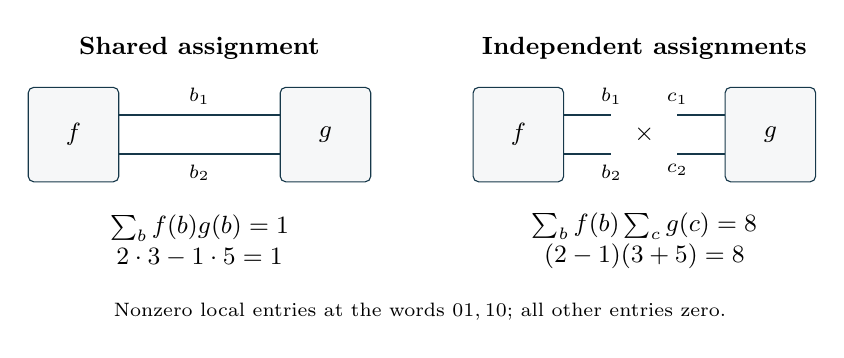
\begin{tikzpicture}[font=\small, factor/.style={draw=navy,fill=navy!4,minimum width=1.15cm,minimum height=1.2cm,rounded corners=2pt}, wire/.style={draw=navy,thick}]
\node[font=\small\bfseries] at (2.35,2.1) {Shared assignment};
\node[font=\small\bfseries] at (8.0,2.1) {Independent assignments};
\node[factor] (fl) at (.75,1.0) {$f$}; \node[factor] (gr) at (3.95,1.0) {$g$};
\draw[wire] ([yshift=2.5mm]fl.east)--node[above,font=\scriptsize] {$b_1$}([yshift=2.5mm]gr.west);
\draw[wire] ([yshift=-2.5mm]fl.east)--node[below,font=\scriptsize] {$b_2$}([yshift=-2.5mm]gr.west);
\node[factor] (f2) at (6.4,1.0) {$f$}; \node[factor] (g2) at (9.6,1.0) {$g$};
\draw[wire] ([yshift=2.5mm]f2.east)--++(.6,0) node[above,font=\scriptsize] {$b_1$};
\draw[wire] ([yshift=-2.5mm]f2.east)--++(.6,0) node[below,font=\scriptsize] {$b_2$};
\draw[wire] ([yshift=2.5mm]g2.west)--++(-.6,0) node[above,font=\scriptsize] {$c_1$};
\draw[wire] ([yshift=-2.5mm]g2.west)--++(-.6,0) node[below,font=\scriptsize] {$c_2$};
\node at (8,1.0) {$\times$};
\node[align=center] at (2.35,-.35) {$\sum_b f(b)g(b)=1$\\$2\cdot3-1\cdot5=1$};
\node[align=center] at (8.0,-.35) {$\sum_b f(b)\sum_c g(c)=8$\\$(2-1)(3+5)=8$};
\node[font=\scriptsize,align=center] at (5.15,-1.25) {Nonzero local entries at the words $01,10$; all other entries zero.};
\end{tikzpicture}
\caption{Signed two-packet control. Sharing both packet IDs retains their common boundary word. Independent summation creates cross terms, even though both local tables are unchanged. The figure illustrates Eq.~\eqref{eq:glue}, not the existence or resource gain of the contracting laws.}\label{fig:shared-boundary}
\end{figure}

The actual J.2 partition consists of heavy singleton pieces and full subtrees rooted at light children. Each nonempty piece has all its crossing tree edges incident to a single node. This strong shape constraint lets the incident-load estimate bound the boundary for one piece. Arbitrary connected pieces do not have it; two adjacent interior vertices of a four-node path have disjoint crossing edges. J.2 additionally pays exceptional terminal bits. Consumed packets can still be present in a local table; the all-copy budget pays their historical use. At the parameter tuple used later, the review records a per-piece cut bound $KT\Lambda/v^{300}$ bits and a total-bit bound $KT\Lambda/k$ that includes additional charged copies and original work. This is a specific bounded-good-outcome construction, not a theorem that any graph partition decreases storage.

The archived signed two-layer control tested all 16 boundary assignments, with outcome contributions $3,-60,50$ summing to $-7$. Deleting the label or terminal marker produced wrong values in negative controls. See \pub{Paper/Tree.lean}{1102}{weighted identity}, \pub{Paper/Pieces.lean}{640}{J.2 quantifiers}, \aud{passes/11c-piece-decomposition.md}{boundary-word reconstruction}, and \aud{passes/14b-tower.md}{the finite controls}.
\interpret{For a human reader, the construction can be viewed as a compiler from one exact weighted network to a sum of controlled network descriptions. Equation~\eqref{eq:glue} explains why the compiler must retain shared IDs; equation~\eqref{eq:load} explains why a value-preserving compiler is not enough without a resource invariant. Neither equation alone implies the full J.4 cutting theorem.}

\section{From weighted programs to a cutter and an accelerator}\label{sec:machine}
\subsection{Weighted computations, accepting bills, and plainness}\label{sec:plain}
The contracting branch uses a nondeterministic tree-program model with ordinary weights from a base ring $A$ and named scalars in a commutative $A$-algebra $R$. Write $\iota:A\to R$ for the coefficient map. An accepting run $r$ has an ordinary weight $w_r$ and an ordered list $b_r$ of requested scalar names, its bill. If $\lambda(q)$ is the scalar named by $q$, its contribution is
\begin{equation}\label{eq:value}
 \operatorname{val}(p,z)=\sum_{r\in\mathrm{Acc}(p,z)}\iota(w_r)\prod_{q\in b_r}\lambda(q).
\end{equation}
The sum is over occurrences of accepting runs, including repeated contributions and zero weights. The empty product is one; an empty accepting-run list has sum zero. The encoded program can request a name and continue independently of the name's scalar value. This is different from using the weight instruction, which multiplies an ordinary coefficient.

A short instance is a description of bounded size. A $T$-plain instance is stronger: the encoded program on the encoded argument halts on every run, all its accepting runs have empty bills, and each accepting run costs at most $T$. The time of executing a caller on that description and the time of the described computation need not be the same. The definition is deliberately not a bound on rejecting-run time. Universal halting is a separate guarantee. The relevant definitions appear in \pub{NS1/Accel.lean}{23}{Accel.lean} and Appendix J/K of \cite{claude}.

\begin{counterexample}[A short halting program need not be plain]
Consider a two-step computation that emits one supported name and then accepts. It halts on all runs and its accepting cost is at most two. Its accepting bill is nonempty, so it is nonplain at every time budget. An operational guarantee cannot alone discharge a value guarantee conditioned on plainness.
\end{counterexample}
The review Lean file \aud{checks/pass15_plain.lean}{pass15\_plain.lean} isolates this counterexample. It is a genuine distinction in the model and will be used in Section~\ref{sec:diagonal}.

\subsection{I.1: weighted simulation is weaker than trace-count bijection}\label{sec:i1}
Proposition I.1 simulates the plain program with a weighted universal automaton under a stated time threshold. The pointer interpreter navigates supported generator prefixes. An unsupported lookup of weight zero may leave an accepting source run with total weight zero, while the corresponding machine branch has no accepting trace. Thus the weighted sum is preserved, but the literal count of accepting occurrences need not be.

\begin{counterexample}[Zero-weight run need not survive simulation]\label{ex:i1}
A minimal example takes the empty name to have weight $-1$ over the integers, every other name zero, and applies the weight instruction to a quoted one-bit false name. The source can accept with weight zero and empty bill. The pointer machine follows supported prefixes and cannot follow the unsupported bit; that branch contributes no accepting trace. The two sums are both zero. In symbols a run list $[0]$ and an empty run list $[]$ have equal sum but different cardinality. This counterexample addresses the stronger wording of the manuscript's simulation, not the scalar identity in the numbered proposition. With a support assumption ensuring that all requested names have valid pointer transitions, the stronger count correspondence may have its intended scope. See \pub{Paper/Universal.lean}{29}{I.1}, \pub{Nc/Uni/EvalU.lean}{251}{pointer branch}, and \aud{passes/publisher-errata.md}{errata item 2}.
\end{counterexample}


\subsection{J.3: one cut, with separate run and value contracts}\label{sec:onecut}
For a fixed parameter tuple the cutter is one program on \emph{every} short description. On any input of size at most $s$, it halts on every run and its accepting outputs are lists of boundedly many bounded-size pieces, with empty bills and a bounded accepting-run clock. Only when the input is plain within the declared budget does the value equation assert that its value equals the weighted sum of products of the pieces' values and that the pieces have the needed plainness. The underlying J.2 network identity is used at the fixed program size, time, and cut parameters. The dealer can omit a tuple with an absent packet at an active wire, because the factor of its incident piece is zero; a present all-zero payload is a different value. Thus the enumeration need not be a bijection between all nominal tuples and accepting runs.

More explicitly, J.3 in the audited formal statement fixes $v$ large, time $\tau\ge v^{a_0}$, $4\lg\tau\le(\lg v)^2$, $s\le\tau$, $2\le k\le v^{64}$, and $\Lambda=(\lg v)^C$, where $\lg$ denotes binary digit length. One program of size at most $v^{a_0}$ serves all such inputs. Accepting runs cost at most $(s+\lfloor\tau k/v^{256}\rfloor)\Lambda$, return at most $k\Lambda$ pieces, each of size at most $(\lfloor s/k\rfloor+\lfloor\tau/v^{256}\rfloor)\Lambda$. For a plain parent, each returned piece is plain at time $\lfloor\tau\Lambda/k\rfloor$. The exact value is the weighted sum of their products. The additive size term permits padding and decoding even when $\lfloor s/k\rfloor=0$.

The reader should not interpret the accepting clock as a deadline for every rejecting execution. Nor should the existence of short pieces alone be taken as evidence of a correct cut. The source constructs a dealer and uses the universal simulation to identify the value of a plain parent. See \pub{Paper/Cuts.lean}{101}{J.3}, \pub{Nc/Dl/Cut.lean}{239}{zero-factor omission}, and \aud{passes/06-one-cut-and-iteration.md}{Pass 6}.

\subsection{J.4: composition, rounding, and the complete cost of a list}\label{sec:cut}
For each accepting parent run of weight $w$ and output list $y_1,\ldots,y_m$, substitute each child's cut expansion into $w\prod_i\operatorname{val}(y_i)$. Distributivity yields one term for every selection of one accepting child run \emph{per occurrence} in the list. The combined weight is the parent weight multiplied by all child weights; the new list is their concatenation. An empty list contributes the parent's weight. If a required child has no accepting run, the product contributes zero. Two repeated child descriptions may select different accepting runs. This identity works over a commutative ring without positivity.

In the audited J.4 scale, write $U=v^H$ with $H=16(a_0+217)\ge272$, and maintain a time bound $T$ and input-size bound $S$. The regular cut takes $k=v^{63}$ whenever $T\Lambda\ge Uv^{64}$; then $T'=\lfloor T\Lambda/k\rfloor$ satisfies $Uv\le T'\le T/v^{62}$. At the terminal cut take $k=\lfloor T\Lambda/U\rfloor+1$, so $2\le k\le v^{64}$ in the declared range, and $\lfloor T\Lambda/k\rfloor<U$. This is a legal final cut even at $T=U$. The size recurrence
\[
 S'=\bigl(\lfloor S/k\rfloor+\lfloor T/v^{256}\rfloor\bigr)\Lambda
\]
ensures $S'v^{48}k\le2cT\Lambda$ if $Sv^{48}\le cT$ and $c\ge1$. Here the padding term is bounded using $k\le v^{64}$; no extra scale factor is needed in this inequality. At a regular step $T\Lambda\le2kT'$ and so $S'v^{48}\le4cT'$. The piece count pays $(k\Lambda)T'\le T\Lambda^2$, and a terminal step uses $kU\le T\Lambda+U$.

The accepting cost of composing cutters with respective bounds $t_1,t_2$ and piece counts $P_1,P_2$ is at most
\begin{equation}\label{eq:listcost}
 t_1+P_1(t_2+62P_2+110)+100,
\end{equation}
with at most $P_1P_2$ pieces. This pays for concatenation and traversal as well as executing the child cutter. Code size is separately bounded by the first program plus three copies of the second plus 3000. Under the J.4 hypotheses, the induction uses $H\alpha$ as a depth bound and absorbs count, time, and size losses $(4\Lambda^2)^{H\alpha+1}$, $(100\Lambda^3)^{H\alpha+1}$, $(8\Lambda)^{H\alpha+1}$ respectively. The logarithmic scale hypothesis makes the largest at most $v$. The resulting common cutter has code size at most $v^H$, its pieces are plain within $v^H$ when the parent is plain, and the advertised bounds are
\[
 t\le\lfloor\tau/v^{24}\rfloor,\qquad
 P\le\lfloor\tau v^2/v^H\rfloor,\qquad
 S'\le v^{H-32}.
\]
Section~\ref{sec:j4tight} records the stronger simultaneous inequalities retained by the review's subsequent formal follow-up. The derivation uses the actual induction witnesses, not an arbitrary abstract cutter satisfying only the weakened interface. See \pub{NS1/Compose.lean}{89}{composition charge}, \pub{Paper/Cuts.lean}{460}{J.4}.

\scope{J.3 and J.4 are encoded publisher results. This audit reconstructed the recurrence, finite controls, and the consumer-facing contract. A complete independent human reconstruction of the instruction-level dealer/listing construction remains distinct from checking the published proof term.}

\subsection{K.2: compile a general circuit into weighted accepting runs}\label{sec:compiler}
The K.2 interface computes the degree-truncated value of a circuit at an encoded word. It does not require the intermediate degrees of the circuit to be bounded. For each gate define $c_g=p_g(0)$ and $q_g(j)=[T^j]p_g(Tu)$. At a product with ordered predecessors $h,v$ and $j\ge1$,
\[
 q_g(j)=c_vq_h(j)+c_hq_v(j)+\sum_{0<i<j}q_h(i)q_v(j-i).
\]
Inductively construct a row $\lambda_g$ on variable addresses and a row $\kappa_g$ on ordered pairs of gate addresses such that, with $a_g=\sum_x\lambda_g(x)u_x$,
\begin{equation}\label{eq:homog}
 q_g(j)=\ind{j=1}a_g+\sum_{l,r}\kappa_g(l,r)\sum_{0<i<j}q_l(i)q_r(j-i).
\end{equation}
Rows are zero at scalars and one-hot for the linear part of a variable. At addition they add. At multiplication set
\[
 \lambda_g=c_v\lambda_h+c_h\lambda_v,\qquad
 \kappa_g=c_v\kappa_h+c_h\kappa_v+\delta_{(h,v)}.
\]
Substitution of earlier recurrences proves \eqref{eq:homog}. Repeated predecessor addresses retain the two ordered sockets. For instance $(1+x)^2$ has degree-one term $2x$, zero in characteristic two but not over the integers. Treating the two references as one contribution would be wrong.

Let $E_g(T)=\sum_{j\ge1}q_g(j)T^{j-1}$. Then
\[
 E_g=a_g+T\sum_{l,r}\kappa_g(l,r)E_lE_r.
\]
For a pending list $L$ and budget $b\ge0$, define $W(b,L)=\sum_{j=0}^b[T^j]\prod_{g\in L}E_g$. Expanding the first factor gives the exact recurrence
\begin{equation}\label{eq:forest}
 W(b,g::L)=a_gW(b,L)+\ind{b>0}\sum_{l,r}\kappa_g(l,r)W(b-1,l::r::L),\quad W(b,[])=1.
\end{equation}
The value through cutoff $d\ge1$ at the output gate is $c_{\rm out}+W(d-1,[\rm out])$. For $d=0$ the constant component suffices. The integer potential $2b+|L|$ decreases by exactly one in either recursive move: a leaf removes one list entry, while a split decrements $b$ and replaces one entry by two. Starting at $2d-1$, it bounds branch length; the pending list has at most $d$ entries. This is the key accounting step. It prices occurrences, not distinct gate indices.

The trie holds coefficient rows and named powers; the program guesses address indices, bills the corresponding values, and uses a balanced access tree for the word. It pays the cost of preparation and padded addresses. For $S\le2^M,N\le2^m$ the source gives an advice-node bound $2^{3M+1}+2^{M+m+3}+3$, height $3M+m+4$, program size $c(M+m+1)+2(d+1)$, and accepting time
\[
 (d+1)(800(M+m)+4000)+(|z|+2)(40m+60)+10m+100.
\]
These are per-accepting-run cost and advice-size bounds, not bounds on the number of branches, total deterministic summation time, or bit cost of arbitrary scalar representations. See \pub{Paper/LowDeg.lean}{42}{K.2}, \pub{Nc/Acc/Loop.lean}{182}{forest recurrence}, and \aud{passes/14c-compiler.md}{compiler reconstruction}.

\subsection{K.3: canonical word encoding and the actual polynomial}\label{sec:k3}
Let $A_t(w)$ be the weighted automaton's fixed-time value for word $w$ of length less than $N$. Its canonical code has one symbol per consumed row, one end mark at row $|w|$, and zeros afterwards. Denote its monomial by $X_{C(w)}$. Two distinct canonical supports are incomparable: a proper prefix has an end marker where the longer word has an ordinary symbol, and non-prefix words disagree at the first unequal symbol. Thus the printed word polynomial
\[
 P(X)=\sum_{|w|<N}A_t(w)X_{C(w)}
\]
agrees with the automaton on each canonical word code. Omitting the end marker would already fail to distinguish a proper prefix from a longer code.

The concrete source constructs a clause polynomial with trailing-row freedom. In the single-input construction traced in the audit it is
\begin{equation}\label{eq:clause}
 Q(X)=\sum_{|w|<N} A_t(w)X_{C(w)}
     \prod_{j>|w|,\ j<N}\left(1+\sum_{\alpha\in\Gamma\cup\{\#\}}X_{j,\alpha}\right).
\end{equation}
The reason is that an accepting run fixes the consumed letters and the first end marker. Each later unused row may be empty or carry one allowed symbol without changing the certificate of that run. Conversely the cumulative input counter forces the used prefix in each contributing certificate. The formal theorem directly requires degree at most $N$ and agreement on every canonical word code, which both expressions satisfy. It is $Q$, not necessarily $P$, that the grid projection and the degree-truncation compiler use.

\begin{counterexample}[Off-code difference, review K.3 erratum]\label{ex:k3}
Take three rows, a binary alphabet, one start/end state, and one step. Give only the transition consuming zero weight one. Write $A=X_{0,0}X_{1,\#}$. The printed polynomial is $P=A$; the clause polynomial is
\[
 Q=A(1+X_{2,0}+X_{2,1}+X_{2,\#}).
\]
On the canonical code of the word 0 both equal one. Turning on a second end marker in row 2 gives $P=1,Q=2$ over the rationals. The formal polynomial identity $P=Q$ is false, whereas equality on canonical codes holds. The example is an actual off-domain test rather than a hypothetical concern about the compiler.
\end{counterexample}
An optional stronger construction adds a zero-weight guard for each pair $p<q<N$ and symbol $\alpha\in\Gamma\cup\{\#\}$, firing when row $p$ has an end mark and row $q$ carries $\alpha$. It eliminates every nonempty trailer. There are $(|\Gamma|+1)N(N-1)$ additional literal occurrences (two per guard), with no new variables. The audit's envelope $1600B^9$ becomes at most $1601B^9$ at its stated $B$. This restores the stronger polynomial identity but is not required by the publisher's construction; the review checked the guarded variant against independent coefficients. The distinction is important: an exact circuit for the concrete projected polynomial is compiled by K.2; only after summing its homogeneous components does K.3 evaluate it on a canonical short plain instance.

The general K.3 theorem fixes $A$, its generating table, $H$, and the grid-completeness factor. For sufficiently large scale $v$, any appropriately bounded target circuit gives one accelerator at that scale, of size at most $v^{C(a+1)}$ when the input gate bound is $v^a$. The same program and trie work for all short descriptions; they cannot depend on the individual input. The hypotheses include the logarithmic scale condition $(\lg v)^{Ca}\le v$ and matrix order at least $v^{B_0}$. See \pub{Paper/CircuitPhi.lean}{175}{clause degree and canonical value}, \pub{Paper/Circuit.lean}{294}{K.3}, \aud{passes/14c-compiler.md}{off-code and guarded constructions}. The external erratum asks that this domain be specified; it does not claim a defect in the proved endpoint.

\section{The diagonal argument: earning the right to substitute a value}\label{sec:diagonal}
\subsection{Two different promises of an accelerator}
An accelerator at scale $v$ has two kinds of guarantee, expressed in Definition K.1. The run guarantee applies to every short description $|z|\le v^{H-32}$: all runs of the accelerator halt, accepting cost is at most $v^{H-16}$, and the named constants lie in its supported table. The value guarantee additionally assumes that the \emph{described computation} is plain within $v^H$. It then equates the accelerator's weighted value with that computation's value. The first promise does not establish the second's domain. This is the central subtlety in K.6.

\subsection{K.4: postponement of named constants}\label{sec:postpone}
Suppose every run of $p$ on an argument halts, every accepting run costs at most $T<2^J$, and all names lie among leaves of a trie of height $\eta$ and size $Q'$. For a vector $e$ with one $J$-bit integer per leaf, define a wrapper $z_e$ that initializes those counters, interprets $p$, decrements a counter for each name request and rejects on failure or underflow. It accepts only if the interpreted run accepts and every counter is then zero. Its own accepting bills are empty. With ordinary accepted weights preserved, the value is
\begin{equation}\label{eq:postpone}
 V=\sum_e \lambda^e\,\iota(\operatorname{sum}(z_e)),\qquad
 \lambda^e=\prod_j\lambda_j^{e_j}.
\end{equation}
This holds by grouping accepting occurrences by their histogram. Supported names imply each original accepting occurrence matches exactly one tally; a missing lookup with value zero may contribute no matching wrapper without changing the weighted sum. A zero-valued supported leaf still has a matching tally. The ordered list of ordinary weights within each matched group preserves duplicate and zero contributions. The wrapper's accepting cost is at most
\[
 (1000+100(\eta+J+1))T+40Q'(J+1)+40,
\]
and its encoded size is bounded by the sizes of interpreter, program and argument plus $4Q'(J+1)+3$. This is a fixed-tally clock. The number of tallies can be exponential. See \pub{Paper/Postpone.lean}{19}{K.4}, \aud{report/pass15-k4.tex}{detailed interpreter proof}.

\begin{example}[Signed cancellation and occurrence counts]
Two accepting runs with the same tally and ordinary weights $1,-1$ have a nonempty matched run list but zero aggregate value. If their common named scalar is $\lambda$, their contributions cancel. Removing the entire group leaves the sum unchanged but loses a different observable. An implementation that needs branch counts rather than only weighted value would require a stronger contract.
\end{example}
The review proves a sharp clock extension in Section~\ref{sec:clock}. The published diagonal only uses the strict clock; it does not depend on this refinement.

\subsection{K.5: transfer to larger scales}\label{sec:scale}
Why transfer scales? Finite-field specialization below supplies a finite table but no bound on its size at the original scale. Instead one retains the constants and amplifies the allowed scale until every requisite description fits. K.5 uses J.4 to speed up the universal pre-evaluator by repeated cuts. It preserves operational promises on all short descriptions and the conditional value promise on plain descriptions; it does not assert that every intermediate program satisfies every auxiliary size predicate of K.1 without checking those fields again.

For $H=16h$, $h\ge17$, and integer $\alpha\ge5$, take $v'=v^\alpha$. For a round lowering the accepting exponent from $f+8$ to $f$, the audited formal budgets use a cutter clock $\tau'=v^{f+9}$, an input allowance $s=v^{\alpha(H-32)+1}$, and the old accelerator at scale $v$. The program guesses a tally, writes its postponed description, invokes the cutter and evaluates every piece in the resulting list. The advertised J.4 bounds give
\[
 t_{\rm list}\le v^{f-15},\qquad
 P\le v^{f+11-H},\qquad
 t_{\rm piece}\le v^{H-16}+30.
\]
The leading product of count and clock is $v^{f-5}$. The additive traversal, guessing, encoding and fixed overhead fit the remaining allowance, giving total per-accepting-run cost at most $v^f$ for the stated parameter range. This does not bound the deterministic work of enumerating every possible output list. The source also bounds code growth per round by $v^{h\alpha+2}+v^{H+1}$, from the initial universal program of size at most $v$.

On the value side the order is different. Plainness of the input permits the pre-evaluation identity; K.4 supplies a plain postponed instance, J.4 supplies plainness and weighted composition of its pieces, and the old accelerator may then use its value guarantee on each piece. All-run halting follows separately because the new program writes the description without evaluating it, and both cutter and old accelerator halt on all short inputs.

After $3\alpha$ rounds the accepting exponent in base $v$ is $H\alpha+1-24\alpha\le\alpha(H-17)$. The code fits $(v')^{4h}$ and the bound on the named power index increases by at most $51h\alpha^2\lg v$. For instance at $h=17,\alpha=5$, the final exponent is 1241, the needed lower endpoint for applying the round is 1240, and the promised endpoint is 1275. These inequalities use the same program and trie throughout the induction. The review checked complete round schedules, repeated pieces, empty products and signed cancellation. See \pub{Paper/Next.lean}{63}{round budget}, \pub{Paper/Next.lean}{270}{scale induction}, \aud{report/pass15-k5.tex}{Pass 15B derivation}.

\subsection{K.6: the self-application, in dependency order}\label{sec:contradiction}
Assume for contradiction that an accelerator of the stated moderate size exists over a nonzero commutative $A$-algebra. The finitely many constants generate a finite-type algebra over the finitely generated base. Reflect the accelerator to that algebra through its injection, then pass to a maximal quotient, a finite field $E$. These maps preserve the syntax, operational bounds, and value equalities; they need not preserve distinct constants. The nonzero field is needed at the last line. Finiteness ensures that the functions $x\mapsto x^{2^j}$ on $E$ have finitely many distinct representatives, with an index reduction $\mathrm{red}(j)$ valid simultaneously for all $x\in E$. K.5 with $\alpha=\max(5,a)$ and then repeatedly $\alpha=5$ produces unbounded compatible scales with the same constant trie and controlled height and exponent bounds. Choose a reached scale $u$ after the finite table is fixed, large enough for the self-query descriptions.

Define a program $P$ on an argument $x$. One branch accepts with weight one. The other guesses a tally $e$, names the scalar $\lambda^e$ using the finite power table, and calls $D$ on the postponed description $z_e$ of $x$ on $x$. Evaluate $x=P$. There are two expansions for the eventual value $V$ of $P(P)$, but they cannot yet be equated. The proof must follow this order:
\begin{enumerate}[leftmargin=1.7em]
\item \textbf{Size first.} Bound the syntax of $P$ and every $z_e$ independently of their values. In particular $|z_e|\le u^{H-32}$ for all guessed tallies. This is a statement about encoded data.
\item \textbf{Run promise.} Apply only $D.\mathrm{run}$ to the short descriptions. Thus $P(P)$ halts on every run, each accepting run costs at most $T=u^{H-15}$, and all requested names are supported in the expanded trie. The actual operational expansion is now
\begin{equation}\label{eq:opdiag}
 V=1+\sum_e\lambda^e\operatorname{val}(D,z_e).
\end{equation}
No correctness guarantee for $D$ has yet been used.
\item \textbf{Plainness.} Choose $J$ with $T<2^J$. K.4 applies to the now justified run list of $P(P)$, gives all-run halting of each $z_e$, empty accepting bills, and a cost bound fitting $uT=u^{H-14}\le u^H$. Equation~\eqref{eq:postpone} gives the separate identity
\begin{equation}\label{eq:otherdiag}
 V=\sum_e\lambda^e\iota(\operatorname{sum}(z_e)).
\end{equation}
These facts prove that every short $z_e$ is also plain in the sense needed by $D$.
\item \textbf{Value promise.} Only now, at the source's first value call in NoAcc.lean line 216, apply $D.\mathrm{val}$ to each $z_e$ using both its size and plainness proof. Thus $\operatorname{val}(D,z_e)=\iota(\operatorname{sum}(z_e))$. Substituting into \eqref{eq:opdiag} and comparing \eqref{eq:otherdiag} gives $V=1+V$.
\item \textbf{Contradiction.} Subtract $V$ in the nonzero field $E$, giving $0=1$. The hypothetical accelerator cannot exist under the hypotheses.
\end{enumerate}
Figure~\ref{fig:diagonal-order} summarizes the order of the preceding obligations.
\begin{figure}[!htbp]
\centering
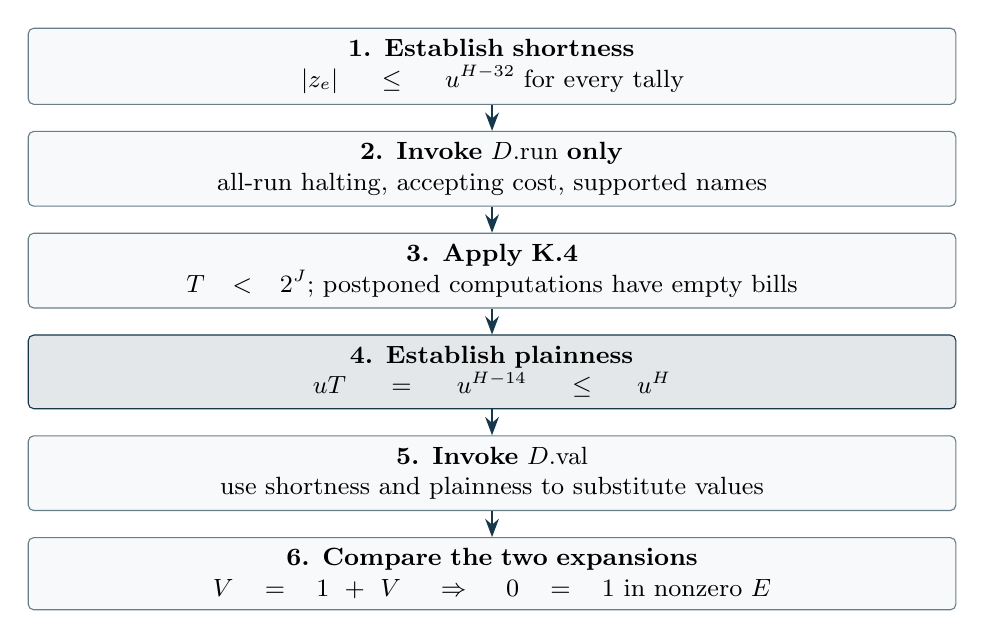
\begin{tikzpicture}[>=Stealth,font=\small, node distance=3.3mm,
 auditstep/.style={draw=navy!65,fill=navy!3,rounded corners=2pt,text width=11.5cm,align=center,inner sep=4pt},
 flow/.style={->,thick,draw=navy}]
\node[auditstep] (s) {\textbf{1. Establish shortness}\\ $|z_e|\le u^{H-32}$ for every tally};
\node[auditstep,below=of s] (r) {\textbf{2. Invoke $D.\mathrm{run}$ only}\\ all-run halting, accepting cost, supported names};
\node[auditstep,below=of r] (k) {\textbf{3. Apply K.4}\\ $T<2^J$; postponed computations have empty bills};
\node[auditstep,below=of k,draw=navy,fill=navy!12] (p) {\textbf{4. Establish plainness}\\ $uT=u^{H-14}\le u^H$};
\node[auditstep,below=of p] (v) {\textbf{5. Invoke $D.\mathrm{val}$}\\ use shortness and plainness to substitute values};
\node[auditstep,below=of v] (c) {\textbf{6. Compare the two expansions}\\ $V=1+V\ \Rightarrow\ 0=1$ in nonzero $E$};
\foreach \x/\y in {s/r,r/k,k/p,p/v,v/c}{\draw[flow] (\x)--(\y);}
\end{tikzpicture}
\caption{Dependency order inside K.6, after specialization and the choice of a reached scale. The operational equality \eqref{eq:opdiag} is available at step 2; the postponement equality \eqref{eq:otherdiag} at step 3. Semantic substitution requires the distinct proof of plainness at step 4. The figure does not assert that a hypothetical accelerator exists.}\label{fig:diagonal-order}
\end{figure}

\interpret{This argument is an indirect diagonalization, rather than a program that literally computes a contradictory value. The assumption of a uniformly correct bounded evaluator is what makes it possible to establish the description's required promise before using its semantic guarantee. A naive self-reference proof that assumes its own plainness would be circular. Here shortness alone supplies the operational handle needed to prove plainness. The two-step nonplain program from Section~\ref{sec:plain} illustrates why one may not skip that step.}
\scope{The pinned K.6 result uses the cutting hypothesis, the common table, finite-type specialization and the scale condition. The review's Pass 15 reconstructed the operational and value contracts and checked five review lemmas against 16 freshly built publisher modules. Neither its finite controls nor the above exposition construct an accelerator. See \pub{Paper/NoAcc.lean}{188}{plainness}, \pub{Paper/NoAcc.lean}{216}{first value use}, \aud{passes/15-diagonal.md}{Pass 15}, \aud{checks/pass15_lean.json}{targeted receipt}.}

\subsection{K.7: the same accelerator must be supplied and denied}\label{sec:match}
A nonexistence theorem at one scale does not exclude an object constructed at a different scale or over a different coefficient structure. Fix the contracting law setting $(A,\theta,H)$ and a candidate circuit for a grid-complete target of order $M$ with size at most $M^a$. At sufficiently large sizes and under the logarithmic bound, the scale lemma chooses $v$ such that
\[
 v^{B_0}\le M,\qquad M^a\le v^{2B_0a},\qquad
 (\lg v)^{(C_2+1)C_1(2B_0a+1)}\le v.
\]
With $d=2B_0a$ and $b=C_1(d+1)$, the one scale pays K.3's $(\lg v)^{C_1d}\le v$ and K.6's $(\lg v)^{C_2b}\le v$. K.3 supplies $\mathrm{HasAcc}(\theta,K,H,v,v^b)$ and K.6 denies precisely that proposition. The source's K.7 chooses the parameters to exclude all candidate sizes up to $2^{c_K(\log_2M)^2/\log_2\log_2M}$ for sufficiently large $M$ and a fixed positive field-dependent $c_K$. The match of field, constants, clock and scale is the bridge from the hypothetical computation to a circuit lower bound. See \pub{Paper/Scales.lean}{141}{matched applications}, \aud{passes/14e-circuit-to-contradiction.md}{whole-chain synthesis}.

\section{Assembling the all-fields and border conclusions}\label{sec:assembly}
\subsection{Uniform exponent, characteristic-dependent threshold}
Choose once for each characteristic an algebraic closure $K$ of the prime field. Proposition~\ref{prop:field} transfers a candidate of the same size over every field of that characteristic into $K$. Apply D.2 there. In a flat field, Section~\ref{sec:flatconvert} yields the explicit rate $2^{(\log_2m)^{4/3}/1600^2}$. In a contracting field write $u=\log_2m$; K.7 gives the stronger eventual exponent $c_K u^2/\log_2u$. For fixed $K$,
\[
 \frac{c_Ku^2/\log_2u}{u^{4/3}/1600^2}
 =1600^2c_K\frac{u^{2/3}}{\log_2u}\longrightarrow\infty.
\]
Thus the same absolute coefficient $1/1600^2$ works in both branches after increasing $m_0(p)$. This order of choices is the reason the universal coefficient does not require a uniform effective classification of fields. The HC projection applies in all characteristics; the permanent projection requires $2\ne0$. This reconstructs the composition from a single arbitrary candidate to the lower bound of Theorem~\ref{thm:main}, conditional on the cited publisher results.

\begin{corollary}[Publisher M.4; exact separation]
For every field $F$, $\VP_F\subsetneq\VNP_F$.
\end{corollary}
\begin{proof}
Propositions~\ref{prop:witness} and \ref{prop:hc} give inclusion and the HC family in VNP. If HC lay in VP, one fixed integer $a$ would bound its gate count by $m^a+a$ for every $m$. Since $c(\log_2m)^{1/3}\to\infty$, for sufficiently large $m$ the lower bound of Theorem~\ref{thm:main} is at least $m^{a+1}\ge m^a+a$. This contradicts its strict inequality.
\end{proof}
The proof is not a lower bound on Boolean truth-table evaluation or on bit complexity of the gate coefficients. It establishes a statement in the algebraic model specified in Section~\ref{sec:model}.

\subsection{What changes in the border proof}\label{sec:approx}
Appendix~\ref{sec:borderdetail} gives the N.1--N.5 derivations supporting the following summary.
The pinned formalization also states and supplies a proof of the corresponding rate for approximating circuits. Section~\ref{sec:border} explains the fixed-size coefficient-field equivalence. Appendix N of the original manuscript supplies additional arguments, so the border separation is not deduced merely by treating the exact theorem as continuous. The audit has formal coverage of the approximate endpoints; its detailed mathematical reconstruction chiefly concerns the exact proof.

In the flat branch, N.3 permits the restriction maps in E.7 to have Laurent-polynomial coefficients. If the sum has no negative powers and constant coefficient $t$, the constant coefficient of its $n$-fold product is $t^{\otimes n}$. At fixed Laurent degree envelope $\Delta$ and fixed number of parties, extracting the coefficient by separate exponent contributions incurs a factor bounded by $(2n\Delta+1)^{|V|}$ in addition to the type count. Taking the $n$th root at fixed parameters removes both polynomial factors, recovering the mixed-cut price comparison. The assumption of no negative powers of the sum is necessary for identifying its constant tensor power with that of the original product. This is the N.3 consumer used by E.10/E.11 for approximation.

The contracting branch is more delicate. Define an approximate accelerator with constants in $R[\varepsilon,\varepsilon^{-1}]$ and value on each short plain instance in $\iota(\operatorname{sum}(z))+\varepsilon R[\varepsilon]$. The operational guarantee is unchanged. Since intermediate factors may have poles, substituting an approximate value into an expression with negative powers could promote a positive-power error to the constant term. Proposition N.4 therefore maintains the error condition by rescaling the parameter. For a round fix a tally $e$ and let $r$ exceed the absolute values of the exponents in its exterior factor $\lambda^e$. Substitute $\varepsilon\mapsto\varepsilon^r$ in the old accelerator. On plain pieces its error now lies in $\varepsilon^rR[\varepsilon]$. Since the negative exponents of the exterior factor have magnitude less than $r$, multiplication leaves a positive-power error. Summing over the cutter's weighted outputs preserves the approximate value guarantee. The trie, exponent envelope, and program size are budgeted under the iterated scale conditions.

At a sufficiently large scale, N.4 constructs an exact accelerator by explicitly extracting the constant coefficient. It guesses bounded named multiplicities and one term of each corresponding power, accumulates their Laurent exponent in a sufficiently wide counter, and uses the interpreter to match the guessed multiplicities to the actual run. A zero exponent sum selects the constant coefficient; the absolute exponent bound prevents modular aliases. The coefficient table becomes a finite set of new constants over the original algebra. The source bounds its size and accepting cost sufficiently to apply K.6, which rules out the resulting exact accelerator. This is the claimed mechanism in the printed proof, whose instruction-level realization is formalized in Lean. A separate human audit of that implementation remains open in our register. The proof may not be replaced by simply discarding all nonconstant scalar terms at the beginning of a computation.

\begin{example}[Why error control must include poles]
An approximation $a(\varepsilon)=1+\varepsilon$ has the same constant coefficient as 1, but multiplying the error by $\varepsilon^{-1}$ introduces a constant one. Rescaling the error to order $r>1$ makes that contribution positive-order again. This is the local reason the N.4 rescaling must exceed the pole budget.
\end{example}
Consequently N.5 supplies an eventual approximation lower bound of the same form as Theorem~\ref{thm:main}. Since HC is in VNP, $\VNP_F\not\subseteq\bVP_F$ for each field. This direction is important: it does not assert that $\bVP_F\subseteq\VNP_F$. Exact computation is a constant degeneration. The publisher separately discusses consequences for determinantal complexity in Remark N.6, explicitly outside the numbered formalized conclusions. We do not treat that remark as a sixth Comparator target. See \pub{Paper/Approximate.lean}{266}{N.5} and the \aud{passes/statement-correspondence.md}{model audit}.

\section{Original local refinements and the status of the errata}\label{sec:extensions}
We collect the review's local mathematical contributions, carefully separating independent proof checks from the public endpoint comparison. The strict denominator-12 bound was proved in Section~\ref{sec:paying}; it is an independent refinement of a scalar budget within the flat case. It does not replace the universal coefficient in the publisher's result. The other two formal refinements are as follows.

\begin{table}[H]
\centering\small
\caption{Review-authored local refinements under the respective pinned hypotheses. These are not changes to the final universal exponent.}\label{tab:local-refinements}
\begin{tabular}{@{}>{\raggedright\arraybackslash}p{.24\linewidth}>{\raggedright\arraybackslash}p{.35\linewidth}>{\raggedright\arraybackslash}p{.33\linewidth}@{}}\toprule
Quantity & Pinned stated bound & Review bound \\\midrule
E.10, $\log_2 L$ & $\ge\ell k^{3/2}/16$ (proof gives $/14$) & $>\ell k^{3/2}/12$\\
K.4 clock premise & $T<2^J$ & $T\le2^J$ (sharp)\\
J.4 listing time & $\lfloor\tau/v^{24}\rfloor$ & $\lfloor\tau/v^{47}\rfloor$\\
J.4 piece count & $\lfloor\tau v^2/v^H\rfloor$ & $\lfloor\tau v/v^H\rfloor$\\
J.4 piece size & $v^{H-32}$ & $v^{H-47}$\\
\bottomrule\end{tabular}
\end{table}

\subsection{A sharp inclusive clock in the postponement interpreter}\label{sec:clock}
The publisher's K.4 assumes $T<2^J$. A $J$-bit unsigned counter represents integers in $[0,2^J-1]$. It is natural to ask whether equality at the clock endpoint is genuinely excluded or merely convenient.
\begin{theorem}[Review K.4 extension, inclusive endpoint]\label{thm:clock}
In the stated K.4 machine and under its other hypotheses, the postponement conclusions and the original wrapper time and size bounds remain valid when $T\le2^J$. The endpoint is sharp uniformly over programs: at accepting clock $T=2^J+1$ a supported-name program can have no matching $J$-bit tally and nonzero original value.
\end{theorem}
\begin{proof}
The structural accepting-run induction establishes $|b_r|+1\le \operatorname{cost}(r)$: the machine pays at least one step beyond its emitted name count. (The exact induction and its use in K.4 are in the review Lean file.) Thus $T\le2^J$ implies $|b_r|\le2^J-1$. Each leaf multiplicity is at most that length, and all original supported accepting occurrences match their unique tally. The wrapper construction, weighted partition and its cost proof remain unchanged. For sharpness take a program with $2^J$ nested requests of the same supported leaf followed by a quote, using the machine's name instructions. Its unique accepting run costs $2^J+1$ and emits exactly $2^J$ requests, so its histogram needs the unrepresentable count $2^J$. Over the integers give the leaf value 2. The original contribution is $2^{2^J}\ne0$, whereas every wrapper with $J$-bit initial counters rejects, making their sum zero. This rules out the next clock uniformly for the same representation.
\end{proof}
This is a strengthening of the stated machine-level tally interface, not a change to the circuit bound. The publisher's diagonal has the strict budget and therefore does not depend on it. The review-authored declarations are in \aud{checks/pass15_plain.lean}{pass15\_plain.lean}; the proof and sharp witness are recorded in \aud{report/pass15-k4.tex}{the K.4 chapter} and \aud{checks/pass15_lean.json}{the targeted Lean receipt}. The proof's positive one-step margin is a resource invariant, not an assumption about a general-purpose interpreter.

\subsection{Simultaneous sharper bounds for the J.4 cutter}\label{sec:j4tight}
The subsequent unnumbered follow-up applies the actual J.4 induction to retain more of its slack. It does not initiate a new numbered pass. Under the same hypotheses as the pinned J.4, the induction gives a common cutter with resource inequalities
\[
 t v^{48}\le \tau v,\qquad Pv^H\le\tau v,\qquad S'v^{48}\le v^H v,
\]
where $t$ is accepting listing time, $P$ is the number of returned pieces, and $S'$ the bound on each piece's encoded size. The construction chooses $H=16h\ge272$ and operates at $v\ge v_0$ with $v>0$. Under these hypotheses the inequalities give the following simultaneous conclusions by natural-number division and cancellation:
\begin{center}
\begin{tabular}{@{}lll@{}}\toprule
Quantity & Advertised J.4 & Review follow-up \\\midrule
Listing clock & $\lfloor\tau/v^{24}\rfloor$ & $\lfloor\tau/v^{47}\rfloor$\\
Piece count & $\lfloor\tau v^2/v^H\rfloor$ & $\lfloor\tau v/v^H\rfloor$\\
Each piece size & $v^{H-32}$ & $v^{H-47}$\\
\bottomrule\end{tabular}
\end{center}
The plainness cutoff and the cutter code-size bound remain $v^H$. These conclusions concern a particular cutter constructed by the proof; they are not implications of the weaker abstract CutHyp alone. The derivation accounts for the same program, the same returned list, and the same cost convention simultaneously.

At the K.5 call $\tau=v^{f+9}$, the stronger bounds give listing time at most $v^{f-38}$ and count at most $v^{f+10-H}$ for $v\ge31$, $H\ge16$, $f\ge38$ and $H\le f+10$, under the two resource inequalities. Combining the latter with $v^{H-16}+30$ gives an upper bound $31v^{f-6}\le v^{f-5}$ for $v\ge31$. This strengthens two cost terms of the existing round, leaving the other overheads and final lower-bound constant unchanged. The two review declarations \texttt{Review.J4.j4\_iterate\_bounds} and \texttt{Review.J4.k5\_listing\_and\_traversal} checked against retained publisher objects with the three allowed axioms. The receipt does not claim a fresh rebuild of those imports or a full new scale transfer. See \follow{followups/j4/README.md}{the unnumbered J.4 follow-up}, \follow{followups/j4/J4_Followup.lean}{Lean source}, and \follow{followups/j4/verification.json}{verification receipt}.

\subsection{Cubic tower word diameter: a reconstruction of the printed strengthening}\label{sec:cubic}
The printed proof of H.1(d) already identifies a cubic bound, while the stated and formal theorem uses exponent seven. We include the reconstruction because it illustrates why balanced composition matters; the cubic estimate is not a new discovery of this review. Fix $h\ge3$ and $R=\F_2[s]/(s^{n+1})$, set $\zeta=1+s$, and use elementary matrices $e_{ij}(a)=I+aE_{ij}$. For distinct $i,m,j$,
\[
 [e_{im}(a),e_{mj}(b)]=e_{ij}(ab),\qquad
 e_{ij}(a+b)=e_{ij}(a)e_{ij}(b).
\]
The generator words on the $h$-cycle provide the required seeds for coefficients 1 and $\zeta$; the wrap carries $\zeta$. A fixed word length $C_h$ covers the seed moves for each ordered pair, using a third index. For powers $\zeta^a$ balanced commutators of exponents $\lfloor a/2\rfloor,\lceil a/2\rceil$ give length at most $C_h4^{\lceil\log_2a\rceil}\le4C_ha^2$. The powers $1,\zeta,\ldots,\zeta^n$ have a triangular coefficient matrix with diagonal one in the $s$-basis; multiplication by the unit $\zeta$ shifts them to a basis indexed by $1,\ldots,n+1$. Arbitrary coefficients therefore require at most $4C_h\sum_{a=1}^{n+1}a^2=O_h((n+1)^3)$ operations in this word model.

Row elimination over the local ring always finds a unit pivot in an invertible remaining block. Characteristic two row exchanges use three elementary operations. Determinant-one diagonal factors can be handled by pairs $\operatorname{diag}(u,u^{-1})$, written using six elementary matrices. The total number of transvections is bounded solely in terms of $h$ (the audit gives $(h-1)(h+9)$). Thus the word diameter is cubic with $h$ fixed. The finite group control at $n=1$ cannot validate this asymptotic exponent; the formal H.1 result retains exponent seven. Either suffices for the consumer H.2. See \aud{passes/14b-tower.md}{cubic derivation} and \pub{Paper/Tower.lean}{25}{the formal H.1 statement}.

\subsection{Disposition of the four textual observations}
\begin{longtable}{@{}p{.13\linewidth}p{.40\linewidth}p{.39\linewidth}@{}}
\toprule
Passage & Finding & Disposition \\\midrule\endhead
K.3 (pp. 56--57) & The clause polynomial can differ from the printed word sum off canonical codes. & State agreement on canonical marked encodings and the degree bound; compile the actual clause polynomial. Counterexample~\ref{ex:k3}.\\[3pt]
I.1 (p. 50) & Unsupported zero-weight lookup can lose an accepting trace. & Preserve the weighted sum; qualify bijection of all accepting runs with the support premise. Counterexample~\ref{ex:i1}.\\[3pt]
H.1(d) (pp. 44--45) & The formal and advertised seventh-power estimate is weaker than the cubic derivation. & Already disclosed in the paper; clarify cross-reference to H.1(d), which H.2 consumes.\\[3pt]
E.10 (pp. 36--37) & The printed and formal arithmetic yield denominator 14, the proposition states 16. & Already disclosed. Our /12 result is an independent local tightening; no change to $1/1600^2$.\\
\bottomrule
\end{longtable}
The first two are the substantive wording qualifications filed in \href{https://github.com/anthropics/formal-math/issues/57}{publisher issue \#57}. They are mathematical counterexamples to stronger interpretations, not objections to the formal endpoints. The upstream issue was open with zero comments when checked on 26 November 2026. Publisher endorsement of our wording has not been obtained. See \aud{passes/publisher-errata.md}{the complete errata note}.

\section{Computational verification and reproducibility}\label{sec:formal}
\subsection{The trust boundary}
A kernel accepts a proof term as inhabiting a formal type relative to its definitions, imports, and foundational axioms. To verify a mathematical claim one must also establish that the type encodes the intended claim. The two checks complement rather than substitute for each other, a distinction emphasized in discussions of machine-checked mathematical proof \cite{pollack}. This review therefore distinguishes (i) source custody, (ii) build and kernel acceptance, (iii) challenge/solution signature correspondence, (iv) mathematical statement reading, and (v) review-authored proofs and finite controls.

The publisher source is pinned at commit \nolinkurl{11b6c7e3c927df2658f513b6b68ea7f8929c62c5}. The source lock records the VP--VNP subtree of 333 blobs, Git tree \nolinkurl{b076b4b081298c4e909bac3f87f0e4462d1fb2cb}, and the 70-page manuscript hash. In preparing this publication manuscript, we independently computed the SHA-256 of the supplied publisher PDF and matched the locked digest
\begin{center}\small\nolinkurl{882f5eefb1e067cc8c99ddfe660c10d1d67f9fcee7b69364bd0bab06c0c1f97c}.\end{center}
The original Lean verification receipts bind Lean 4.33.1 \cite{lean4} and nine external dependency revisions (including mathlib \cite{mathlib} at \nolinkurl{0df444a360eaa60ab8c11dca51a86af692955474}); prebuilt external library objects are part of their stated trust input. The source lock and exact workflow record the project code and checker. Comparator \cite{comparator} compares the exported declarations and invokes the kernels, including nanoda \cite{nanoda}; the pinned exporter and sandbox revisions are recorded in the \follow{reproduce/versions.env}{verifier lock}. We do not claim to have rebuilt mathlib from source during that review.

\subsection{Five endpoints, isolated imports, and the permitted axioms}
The trusted challenge imports Statement alone (which imports Mathlib), declaring the five required types using placeholder proofs. The proof-bearing Solution imports Statement and the relevant proof modules, not the challenge. Importing both in one environment merely to find a theorem name would be an inadequate verification. The archived native execution reads the two sets of types in isolated environments and compares the full signatures; the separate Comparator execution compares the public challenge and solution and checks the exported proof. The permitted foundational axioms are propositional extensionality (\texttt{propext}), quotient soundness (\texttt{Quot.sound}), and classical choice (\texttt{Classical.choice}).

\begin{center}
\begin{tabular}{@{}p{.36\linewidth}p{.54\linewidth}@{}}\toprule
Configured declaration & Encoded conclusion \\\midrule
\texttt{Solution.mainTheorem} & Exact HC over every field and permanent over fields of characteristic $\ne2$.\\
\texttt{Solution.separation} & Proper inclusion of VP in VNP over every field.\\
\texttt{Solution.mainTheoremApprox} & Laurent-series approximation of HC over every field and of permanent in characteristic $\ne2$.\\
\texttt{Solution.separationClosure} & VNP not contained in the defined border VP for every field.\\
\texttt{Solution.permanent\_over\_real} & Exact permanent specialization over the real field.\\
\bottomrule\end{tabular}
\end{center}
The approximate and exact public predicates quantify their positive rate constants separately; the supplied proofs admit the same explicit choice. The distinction between statement-level equivalence and kernel acceptance is especially relevant for the formal border convention. See \aud{passes/14d-formal.md}{Pass 14D} and \aud{passes/statement-correspondence.md}{the public-model audit}.

\subsection{Recorded executions and independent extensions}
The table identifies the historical executions. The paragraph below records which checks the review team repeated for version 1.1.
\begin{longtable}{@{}>{\raggedright\arraybackslash}p{.25\linewidth}>{\raggedright\arraybackslash}p{.39\linewidth}>{\raggedright\arraybackslash}p{.28\linewidth}@{}}\toprule
Recorded execution & Result and scope & Evidence \\\midrule\endhead
Complete native build (Pass 14) & 324 publisher Lean sources (323 distinct modules of four default targets plus reporting script) compiled; 5/5 full signature matches; 22 axiom reports and 10 intermediate type readbacks. External libraries pinned, prebuilt. & \aud{checks/pass14_release.json}{Native receipt}; \aud{checks/pass14_release.py}{runner}.\\[3pt]
Linux Comparator & Review-team GitHub Actions run 45691617731, job 139478246305; default targets and unmodified publisher driver; all five configured declarations accepted, nanoda enabled. & \href{https://github.com/nousentllc/VP-VNP-Review/actions/runs/45691617731}{Run}; \aud{checks/pass14_comparator.json}{receipt}.\\[3pt]
Review /12 bound & Scalar and circuit-level refinement checked against the exact freshly built Paper.Rate object. Not a publisher Comparator endpoint. & \aud{checks/pass14a_circuit_results.json}{Circuit receipt}.\\[3pt]
Pass 15 targeted build & 16 publisher modules rebuilt for NoAcc, eight publisher declarations and five review lemmas queried. K.4 clock and plainness distinction. & \aud{checks/pass15_lean.json}{Targeted receipt}.\\[3pt]
Release-candidate Tier 0 & Stored source/receipt checks and 24 finite controls; outside AI reader reported successful Tier 0 replay. & \follow{REPRODUCE.md}{Reproduction guide}; \follow{reconciliation/release-candidate.md}{candidate record}.\\[3pt]
Native Tier 1 candidate & 23 review Lean modules checked on macOS against retained pinned publisher objects; expected evidence hash matched. & \follow{reconciliation/release-candidate.md}{candidate record}.\\[3pt]
Unnumbered J.4 check & Two review declarations accepted against retained publisher objects, with permitted axioms. No fresh publisher rebuild in this follow-up. & \follow{followups/j4/verification.json}{follow-up receipt}.\\
\bottomrule\end{longtable}
The original archived Linux build and the new Docker reproduction entry points are different evidence. The latter had not received a fresh Linux replay in the release record. A separate outside operator has not yet independently executed Tiers 1 and 2. The external AI critique (Claude Opus 5.5, reported model ID \texttt{claude-opus-5-5}) provided six observations and a follow-up Tier 0 check. It is not an independent human assessment or a second full kernel reproduction.

\paragraph{Checks repeated for version 1.1.}
On 26 November 2026 the review team ran Tier~0 in clean exports of
\href{https://github.com/nousentllc/VP-VNP-Review/tree/f726d3a7608e31b5c88804764b6e65c203179d42}{the tagged candidate}
and \href{https://github.com/nousentllc/VP-VNP-Review/tree/f7d16f5fd48ac0ffcfe50c3828778dc7c97a27c3}{the current review snapshot},
and in the extracted v1.0 software deposit. Each replay checked custody of the 333-blob publisher tree, historical receipt consistency and the 63-entry claim map, and reproduced the 24 finite controls. The same controls ran on three copies of the evidence. The 530 selected source and evidence files agree byte for byte across the deposited software, the report bundle and the review snapshot.
The team also reran Lean on the two J.4 review declarations with the pinned, retained publisher imports. Each returned the three axioms listed above. This targeted elaboration checks the added J.4 results. The last complete five-endpoint Lean/nanoda comparison remains the archived Linux job in the table.
The historical Tier~2 transcript verifier reproduced its expected evidence digest and rejected a control transcript with the nanoda success marker removed. It checks the contents of a recorded run. The supplemental publication examples also reproduced their saved values, including 72 integer J.4 cases. The publication ZIP supplies the programs, fresh receipts and input pins.

\subsection{Receipt reconciliation and negative controls}\label{sec:receipts}
The external review identified that the comparator transcript's build counts had been mixed. Edition 12 traced all 14 quoted lines to their actual sources. The 9,032 figure belongs to the outer build; 8,708 and 9,027 belong to the two inner Comparator builds. These are build-job counts, not numbers of mathematical lemmas, and host-specific logs need not reproduce those counts. The provenance correction leaves the exact acceptance markers intact. See \aud{reconciliation/edition12-comparator-and-margin.md}{log and margin reconciliation} and \aud{reconciliation/edition12-external-review.md}{response to all six observations}.

A second concern is the separation of the intentional placeholders in Challenge from the proofs. The original workflow inherited a filter recognizing single quotes, whereas Lean's diagnostics can enclose \texttt{sorry} in backticks. The review separately scanned the complete recorded native and Linux transcripts, finding exactly the five intended Challenge warnings per build and none outside Challenge. The maintained parser accepts both quote styles. This is a repair to diagnostic coverage, not an assertion that the original workflow alone checked every possible failure mode. The proof-side axiom readbacks and the actual Comparator acceptance remain separate evidence. See \aud{checks/pass14_warnings.py}{warning parser}.

The independent finite controls were used to falsify weakened assumptions, not to estimate the probability that an unbounded theorem is correct. Their most informative role is to separate mathematically valid transformations from incorrect simplifications. For example, the two-cut rank test detects selection of independent witnesses; the boundary-word test detects deletion of a common label; the two-step program detects shortness without plainness. None of these constructs the spectral point or hypothetical accelerator required for the theorem. Appendix~\ref{app:matrix} maps these controls to the 63-claim register.

\section{Implications for mathematical understanding and computational representations}\label{sec:implications}
We draw three methodological lessons from the audit. These observations are not new complexity-theoretic corollaries.

\subsection{A global observable determines the information that must survive local composition}
The identity $Z=\sum_b\prod_jV_j(b)$ shows that local sufficiency must be qualified by the admissible shared boundary. An independent summation over each region generally computes a different function (Section~\ref{sec:glue}). This is why the proof tracks shared packet identities and the scope of local rewrites. The weighted identity is established for the publisher's model; transfers to other computational models require separate hypotheses and proofs.

\subsection{A recursion is more than its local register budget}
The accepting cost of one K.5 round is a sum of listing cost, count times per-occurrence cost, and overhead. The number of accepting computations is not controlled by that bound. Likewise a finite cut with small boundary may use expensive preprocessing, multiple historical copies, or a large installed table. The review retains those distinctions because they are needed by different downstream consumers. A proposed deterministic algorithm cannot claim the same bound merely by substituting exhaustive enumeration for a guessed branch. The interpretation is a general discipline for reading recursive resource proofs; it is not a theorem transferring the publisher's lower bound to memory or other computational models.

\subsection{An equality is only as strong as its observational domain}
The K.3 clause example makes the domain of equivalence explicit. Two representations agreeing on canonical codes need not agree as formal polynomials. The I.1 example makes the choice of observable explicit: weighted value is not trace count. And K.6 shows the order in which an operational guarantee may be used to establish a semantic precondition. We summarize this as a conditional interface principle: if an operation is defined only on a domain $D$, equivalence of representations on $D$ may be substituted only after proving that the next operation stays inside $D$ and preserves its other required resource and type hypotheses. If the domain expands, the old equality may fail. The counterexamples in this paper provide motivation, not an independently established general architecture or lower bound. A separate research program may test such transfers.

\section{Limitations, open obligations and independent review}\label{sec:limits}
The central verification finding is that the five \emph{encoded} statements were accepted in the recorded proof checks against the pinned definitions and axiom policy. Their correspondence to conventional nonuniform arithmetic complexity is separately analyzed in Section~\ref{sec:model}. A named independent human reader of the statement is still desirable. The following questions are explicit limitations rather than invitations to expand the numbered review indefinitely:
\begin{enumerate}[leftmargin=1.7em]
\item \textbf{Geometry and duality.} The existence of the full G.2 law family depends on the upstream CAT(0) price geometry and the detailed F.2--F.5 contraction/near-orthogonality results. Appendices~\ref{sec:geometricdetail} and \ref{sec:windowdetail} reconstruct the completion, toolkit and F.1--F.5 route as well as the final uniformity comparison. This is explanatory source review; independent expert verification of every step remains pending, and finite group tests do not establish the upstream assumptions.
\item \textbf{Machine-level reading.} J.3/J.4's concrete dealer, listing program and every instruction-level overhead have formal coverage, but our human-oriented reconstruction does not rederive every subroutine. The J.4 follow-up strengthens the simultaneous bounds from retained induction witnesses; it is not a different proof of the full separation.
\item \textbf{Approximate computation.} The border endpoints passed formal comparison. Appendix~\ref{sec:borderdetail} develops N.2/N.3, the round invariant, exponent growth and constant-coefficient extractor of N.4; the complete approximate-accelerator implementation is a separate human-reading task. In particular there is no claim about coefficient bit cost or every possible topology-based closure.
\item \textbf{Reproduction.} The publisher-source and review-team checks share the formal definitions and foundational axioms. A fresh independent outside-operator execution of the tagged Docker Tiers 1/2 and an independent human statement-level assessment remain pending. The two-kernel evidence does not establish a field-wide consensus or eliminate all possible trusted-base failures.
\item \textbf{Scope of refinements.} The strict /12 scalar estimate, inclusive K.4 clock, and J.4 bounds are local. No claim is made that the first is an optimal geometric constant, the second is a general interpreter bound, or the third improves the final circuit exponent. The H.1 cubic estimate is already described in the publisher manuscript.
\end{enumerate}
The public review invitation \href{https://github.com/nousentllc/VP-VNP-Review/issues/1}{issue \#1} solicits a human expert's independent reading of the precise formal definitions, characteristic exception, quantifier order and approximation convention. The upstream wording issue is likewise not represented as resolved. The conclusions are limited to the recorded verification and the stated mathematical reconstruction.

\section{Conclusion}\label{sec:conclusion}
The AI-assisted statement reading finds correspondence with the publisher's stated algebraic model, with precise qualifications about approximation and nonuniform circuit cost. Independent human assessment of that reading remains pending. The recorded review-team native build and two-kernel Comparator execution document acceptance of the five encoded statements at the pinned revision under the recorded trust assumptions; this is not outside-operator reproduction or an independent proof of the separation. Our dependency-ordered reconstruction explains how the geometry of prices, balanced extraction, shared selectors, weighted tensor laws, cutting and diagonalization are connected. The strongest lesson is not a new claim about general complexity: it is that value preservation is an interface property, and its use requires the same shared data, same hypotheses, and explicitly matched resources.

The review's independently derived counterexamples make the two exposition qualifications precise. Its local mathematical refinements strengthen the flat scalar estimate, the inclusive postponement clock, and the cutter's simultaneous resource bounds within their original hypotheses. Those results have their own proofs and verification receipts, and should be cited as review contributions rather than credited as the origin of the VP--VNP separation. The historical audit and its evidence remain available as supplementary records.

\section*{Research contributions and AI disclosure}
\addcontentsline{toc}{section}{Research contributions and AI disclosure}
Justin Candler directed the research and defined its objectives. Uriel, the project's AI research agent operating through OpenAI Codex and ChatGPT, contributed mathematical reconstructions, finite controls, Lean checks, manuscript preparation and evidence reconciliation. The release-candidate tooling records GPT-6.2; a complete model inventory for earlier passes is unavailable. Claude Opus 5.5 (reported model identifier \texttt{claude-opus-5-5}) contributed the external AI critique and Tier 0 follow-up. This contribution is not independent human peer review. Additional user-supplied feedback from DeepSeek informed the final presentation and scope language; no kernel reproduction is attributed to that editorial review. The claimed separation and its supplied formalization are attributed to Claude and Anthropic \cite{claude}.

\noindent\textbf{Data and code availability.} The repository contains the pinned publisher source, verification receipts, review code, finite controls, and historical technical report. The claim dossier in Part II (p.~\pageref{part:dossier}) preserves the 63 claim-level entries and their evidence boundaries; the machine-readable register is available at \aud{report/proof-coverage.csv}{proof-coverage.csv}. Publisher material retains its upstream license and notices. Independent human statement assessment and outside-operator Tiers 1 and 2 remain pending.

\appendix
\section{Technical derivations: spectral geometry and the field alternative}\label{sec:geometricdetail}
This appendix gives the algebraic and metric arguments supporting Sections~\ref{sec:geometry} and \ref{sec:flat}. These are explanatory reconstructions of the pinned publisher proof; formal verification and the limits of independent mathematical review are reported in Sections~\ref{sec:formal} and \ref{sec:limits}.

\subsection{Wire exponents, co-located labels, and the actual hub maps}
For a nonempty set of parties $P$, put $a(q)=\varphi(\langle q\rangle_P)$. Restriction and the scalar unit imply $1\le a(q)\le q$, while multiplication gives $a(qq')=a(q)a(q')$. Monotonicity then forces a power law. To see the last step explicitly, for integers $p,q>1$ compare $p^n$ with $q^{\lfloor n\log_qp\rfloor}$ and $q^{\lfloor n\log_qp\rfloor+1}$. Apply $a$, take logarithms, divide by $n$, and let $n$ grow. It follows that $\log a(p)/\log p=\log a(q)/\log q$. Thus $a(q)=q^g$ for one $g\in[0,1]$. A singleton has $g=0$, since its nonzero unit tensor is equivalent by restriction to the scalar unit.

The triangle inequality for wire exponents is also an actual local map. From the wires $\langle q\rangle_{uv}\langle q\rangle_{vw}$ contract the two indices at $v$ by the equality pairing. The result is $\langle q\rangle_{uw}$. Restriction monotonicity gives $q^{d(u,w)}\le q^{d(u,v)+d(v,w)}$ for $q>1$, hence $d(u,w)\le d(u,v)+d(v,w)$. The same construction along a spanning tree bounds a multiparty diagonal exponent by the sum of its edge distances. The tree estimate is part of the publisher's toolkit, although the public endpoint route does not require every clause of every packaged theorem.

For the hub lemma, write the coefficient tensor as $t(x,y)=\sum_{j=1}^{L}\alpha_j(x)\beta_j(y)$. Copy every coordinate of $x$ to the first hub and every coordinate of $y$ to the second. A dimension-$L$ middle wire provides one common $j$. Contracting the first hub with $\alpha_j(x)$ and the second with $\beta_j(y)$ yields exactly $t$. The middle index is not two independent choices. If hubs are mapped onto existing party labels, the local linear maps at the merged site multiply and contract all their distinct logical legs. Ordinary restriction allows this. A consumer that requires identity maps at the original ends should first retain distinct logical end and hub labels and only pull back the geometric placement; physical coincidence alone does not make every local map an identity. Pass 12D tested 116 placements and 600 entries, including such coincidences, but the formula supplies the general argument. See \aud{passes/12d-hub-routing.md}{the hub-routing reconstruction}.

\subsection{The crossing coefficient is an integral object, not merely a rank estimate}\label{sec:crossdetail}
The B.2 family is more informative than the statement that two unrelated flattenings have small rank. It gives one integral coefficient tensor and two decompositions of it, with complementary degree budgets. Here is the algebra behind that fact. Write $y=X^2$ and define integer polynomials
\[
 B(r,n)=[t^n]\frac{(1+t)^r}{(1+yt)^{r+1}},\qquad
 C(r,n)=[t^n]\frac{(1+yt)^r}{(1+t)^{r+1}}.
\]
Then $C(r,n)=y^n B(r,n)|_{y\mapsto y^{-1}}$. With $\beta_r(t)=(1+t)^r/(1+yt)^{r+1}$, multiplication of the finite geometric sum gives
\[
 (1-yts)(1-y)\sum_{r<R}y^r\beta_r(t)\beta_r(s)
 =1-y^R(1+yt)(1+ys)\beta_R(t)\beta_R(s).
\]
Comparison of the coefficients of $t^i s^j$, modulo $y^R$, yields
\[
 (1-y)\sum_{r<R}y^rB(r,i)B(r,j)\equiv [i=j]y^i\pmod {y^R}.
\]
This is a finite congruence in a formal power-series ring. It uses no analytic convergence, positive-definite scalar product, or division in the final coefficient ring. It is consequently available before specializing the integer coefficients to any field.

For four symbols $s_a=(I_a,J_a)$ and similarly $s_b,s_c,s_d$, arrange rows and columns in party order $a,d,c,b$. The publisher's matrix has diagonal party blocks zero and the following entries at row index $i$ and column index $j$:
\[
\resizebox{\linewidth}{!}{$\displaystyle
\begin{pmatrix}
0&C(i,j)&[i=j]X^{2i+1}&(y-1)X^{2i+1}B(i,j)\\
-C(j,i)&0&X^{2j+1}B(j,i)&-[i=j]X^{2i+1}\\
-[i=j]X^{2i+1}&-X^{2i+1}B(i,j)&0&-(y-1)C(i,j)\\
-(y-1)X^{2j+1}B(j,i)&[i=j]X^{2i+1}&(y-1)C(j,i)&0
\end{pmatrix}. $}
\]
Each displayed entry represents a block indexed by the corresponding finite sets; it is not a single four-by-four scalar matrix unless those sets are singletons. Let $\Psi(X)$ be its determinant. At $X=1$ the factors $y-1$ vanish and the remaining inter-party blocks force the matching of the two symbols, with a sign depending only on their sizes. Exchanging the two sets in the appropriate symbols and absorbing that fixed sign gives the two-wire tensor when the coefficients of $\Psi$ are summed.

To bound the coefficient at degree $N$, choose $R=N+1$. The congruence just proved factors the two off-diagonal pair blocks modulo $X^{2R}$ through the diagonal matrix $D=\operatorname{diag}(X^{2r+1})_{r<R}$. A Schur-complement enlargement reduces the determinant to an expansion in choices of rows from two such diagonal blocks. A surviving choice is a pair $(T_1,T_2)$ with equal cardinalities. Unequal cardinalities leave a rectangular zero-coupled block and therefore give determinant zero. An equal-cardinality choice contributes
\[
 X^{E(T_1,T_2)} A_{T_1,T_2}(s_a,s_d;X)
                         B_{T_1,T_2}(s_b,s_c;X).
\]
Only choices with $E(T_1,T_2)\le N$ survive at degree $N$. There are at most $P(N)$ such Frobenius symbols. Splitting the residual degree $N-E$ between the two factors costs at most $N+1$ possibilities. Hence this very coefficient has an $AD\mid BC$ decomposition with at most $(N+1)P(N)$ products. The sign in the explicit printed-order minor expansion is part of the factorization, rather than a positivity assumption; the review's equal-rank parity reduction has $d^2-d$ even.

The reciprocal identity supplies the other cut. Apply $X\mapsto X^{-1}$, rescale the rows and columns by the prescribed monomials, and interchange $b,d$. The products of the row and column multipliers have total $X$-degree $\Theta=2(e_1+e_2)$. The factors $(y-1)^{2n_2}$ and $(1-y)^{2n_2}$ cancel as polynomial factors. Rows and columns undergo the same permutation, so their permutation signs multiply to one. The result is
\[
 X^\Theta\Psi(X^{-1};s_a,s_b,s_c,s_d)
       =\Psi(X;s_a,s_d,s_c,s_b).
\]
In particular $\deg\Psi\le\Theta$. Its degree-$N$ coefficient has the second cut decomposition bounded by $(\Theta-N+1)P(\Theta-N)$. The identity precedes specialization; coefficient cancellation in characteristic two does not invalidate it. The archived checks use four signed determinant instances and an independent finite coefficient family. They neither establish an unbounded determinant identity by enumeration nor certify the review's explicit sign convention as a separate Lean theorem. See \aud{passes/12d-counting-and-minors.md}{Pass 12D} and publisher Appendix B.3.

\subsection{Why the counting error is uniform in the chosen coefficient}
The partition-counting background is classical (\cite{andrews,hardyRamanujan}); here the relevant uniformity concerns the coefficient chosen after evaluating the tensor.
The selected $N$ in B.3 depends on the spectral point and the large energy. A pointwise lower asymptotic at that $N$ would be unsafe, particularly when $N=0$. The proof instead uses the lower asymptotic only at the two initial energy budgets $E_1,E_2$, where it finds large classes of fixed size and energy. At every possible output index it uses the global bound $\log P(N)\le\kappa\sqrt N$. Polynomial losses such as $(E_i+1)^2$, $N+1$ and $\Theta+1$ have logarithms $O(\log n)$ uniformly for $0\le N\le\Theta=O(n)$. After division by $\sqrt n$ these losses vanish uniformly, including at zero.

A normalization detail deserves its own argument. The interleaving injection proves $P(k^2E)\ge P(E)^k$ for every $k$. With $E_0$ chosen near the supremum of $\log P(E)/\sqrt E$, take $k=\lfloor\sqrt{E/E_0}\rfloor$. Then
\[
 \frac{\log P(E)}{\sqrt E}\ge
 \left(1-\sqrt{E_0/E}\right)\frac{\log P(E_0)}{\sqrt{E_0}}.
\]
This proves a full limit, not just a subsequential lower bound. For the review's explicit constant, let $A(E)=P(E)$ and let $Z(t)$ count exact energies. Partial summation gives $Z(t)=t\int_0^\infty e^{-tx}A(x)\,dx$ with the initial atom incorporated by the integral convention. The upper and lower growth envelopes $\exp((\kappa\pm\eta)\sqrt x)$, outside a fixed compact interval, imply $t\log Z(t)\to\kappa^2/4$ by maximizing $-tx+\kappa\sqrt x$; restricting the lower integral to a small interval around its maximizer gives the matching lower bound. Frobenius symbols of energy $2n$ are partitions of $n$, so
\[
 Z(t)=\prod_{j\ge1}(1-e^{-2tj})^{-1},\qquad
 t\log Z(t)=\sum_{r\ge1}\frac{t}{r(e^{2tr}-1)}\longrightarrow
 \sum_{r\ge1}\frac1{2r^2}=\frac{\pi^2}{12}.
\]
The passage through the sum follows from $e^u-1\ge u$ and summability of $1/(2r^2)$. Thus $\kappa=\pi/\sqrt3$ for natural logarithms. The publisher only needs a common positive $\kappa$; this additional normalization is a review derivation, not a newly formalized endpoint.

\subsection{The invariant mean and its order of limits}
For fixed $T$, the fan construction produces a sequence of prices on two copies of $\mathbb Z^2$. A common bound $W_n(P,P+g)\le K\|g\|_1$ holds for each fixed displacement $g$. Average over the two-sheet rectangles $0\le i<n^2$, $0\le k<n$, then take one fixed free-ultrafilter limit. For a bounded function sequence and fixed translation, the proportion of points affected by the boundary tends to zero. Thus the mean is translation invariant. No assertion that the individual fan geometries converge ordinarily is needed.

Set $\nu(g)^2=\mathbb E W(P,P+g)^2$. Translation invariance and Minkowski give evenness and subadditivity. Fekete's lemma yields $N(g)=\lim_{S\to\infty}\nu(Sg)/S=\inf_{S\ge1}\nu(Sg)/S$, a homogeneous seminorm on integer vectors. Apply the scalar crossing display pointwise with the two local wire distances as its weights, average, and use Cauchy--Schwarz on the products of distances. Then scale all eight fixed vectors by $S$ and pass to $N$. The same positive Young parameter is retained throughout this step.

For completeness, the last parallelogram argument uses long vectors $A_i=R^2(a+b)+i(a-b)$ and $B_i=R^2(a-b)+i(a+b)$ for $0\le i<R$. Apply the symmetric crossing inequality at these vectors and again after subtracting $a$. The bounded first-difference terms telescope when averaged over $i$. Convexity of a seminorm controls the remaining long-direction differences, leaving
\[
 N(a+b)^2+N(a-b)^2\le 2N(a)^2+2N(b)^2+O(R^{-1}).
\]
Let $R\to\infty$. Applying the resulting inequality to $a+b,a-b$ and using integer homogeneity gives the reverse inequality. This is the complete logical role of C.2 in the later fan endpoint. The order is fixed fan parameter, fixed displacements in the finite-box mean, homogenization, the long-vector comparison, and then the endpoint's successive $A\to\infty$ and $T\to\infty$. Taking $A=T$ is not justified by the preceding error estimate.

\subsection{Completion must produce one midpoint for every test point}\label{sec:completiondetail}
A quantifier distinction can be hidden by the phrase ``the CN inequality holds.'' The needed assertion is that for each endpoint pair there exists one midpoint satisfying the inequality for all test points. Choosing a new midpoint after seeing the test point gives a different condition.

Add a fresh midpoint label for every pair in $V_j$ by A.8, obtaining an extending price on $V_{j+1}$. The two upper half-distance bounds and the triangle inequality force exact equality on the two legs. Every finite collection of labels in $\bigcup_jV_j$ lies in one stage, so the union has a price. Quotient zero-distance labels and take its metric completion $Y$. To show that its metric is a price, fix finitely many points $y_1,\ldots,y_q$ and approximate them by old points $x_{i,n}$. The bound
\[
 |d(x_{i,n},x_{j,n})-d(y_i,y_j)|\le d(x_{i,n},y_i)+d(x_{j,n},y_j)
\]
is uniform over the finite set of pairs. Each old distance table is a price and the set of price tables is closed under pointwise limits. Repeated labels and zero distances cause no problem, since the argument is on finite pullbacks rather than on injective placements.

Now choose $x_n\to x$, $v_n\to v$ in the dense union and an old midpoint $m_n$. Put $D_n=d(x_n,v_n)/2$ and $\epsilon_{nk}=d(x_n,x_k)+d(v_n,v_k)$. The CN inequality for $m_n$ at $m_k$ gives
\[
 d(m_n,m_k)^2\le \tfrac12d(m_k,x_n)^2+\tfrac12d(m_k,v_n)^2-D_n^2.
\]
Both first distances are at most $D_k+\epsilon_{nk}$ and $|D_n-D_k|\le\epsilon_{nk}/2$. Since the $D_k$ are bounded, the right side tends to zero. Thus the midpoints are Cauchy; their limit $m$ has the two required half-distances. Taking limits in CN at each fixed $z\in Y$ proves its inequality for that same $m$. Completeness now supplies the intended CAT(0) structure. This fills a reading obligation recorded in the old C.3 row at the level of the mathematical argument; it adds no new kernel receipt.

\subsection{The CAT(0) toolkit and the rigid cube}\label{sec:toolkitdetail}
For general metric geometry background, see \cite{bridsonHaefliger}; the specialized rigidity argument below follows the publisher.
The toolkit's common engine is strong midpoint convexity. Suppose a continuous nonnegative $G$ on a nonempty closed midpoint-convex subset satisfies
\[
 G(m)\le\tfrac12G(q)+\tfrac12G(q')-\tfrac c4d(q,q')^2,\qquad c>0.
\]
A sequence approaching $\inf G$ is Cauchy by this inequality, so it has a minimizing limit $b$. Starting with $G(y)\ge G(b)$, apply the inequality at the midpoint of $b,y$. If $G(y)\ge G(b)+c'd(y,b)^2$ is known everywhere, the midpoint argument improves the coefficient to $(c+c')/2$. Iteration from $c'=0$ gives $G(y)\ge G(b)+c d(y,b)^2$. Applied to sums of squared distances this yields barycenters; applied to distance from a fixed point on a closed convex subset it yields the projection inequality.

Taking weights $1-t,t$ at two endpoints produces the geodesic point at parameter $t$ and the inequality
\[
 d(z,\gamma(t))^2\le (1-t)d(z,x)^2+t d(z,v)^2-t(1-t)d(x,v)^2.
\]
For the quadrangle estimate, apply this to a point on $[y,u]$, bound $d(x,v)$ through that point, and optimize its parameter. The result is
\[
 d(x,v)^2+d(y,u)^2\le d(x,u)^2+d(y,v)^2+2d(x,y)d(u,v).
\]
The weaker diagonal-versus-side sum follows from $2ab\le a^2+b^2$; equality in that weaker inequality forces opposite sides to agree. These equality consequences, rather than the weak inequality alone, are what D.2 consumes.

To fill a rigid rectangle, define
\[
 \Phi(p,p';r,r')=d(p,r')^2+d(p',r)^2-d(p,r)^2-d(p',r')^2.
\]
The quadrangle estimate bounds it by $2d(p,p')d(r,r')$. If opposite sides of the original rectangle have lengths $\delta,h$ and both squared diagonals equal $\delta^2+h^2$, splitting its two length-$h$ sides at parameters $s,t$ decomposes $\Phi$ into four terms. Their upper bounds sum to the already attained total $2h^2$, hence each is attained. First set $s=t$ to show the equal-height segments have length $\delta$. Then the geodesic inequalities and the attained four-point identity give
\[
 d(a,b)^2=\delta^2+h^2(s-t)^2.
\]
This permits filling a cube coordinate by coordinate, preserving every pairwise distance, not only edge lengths.

There is no inference here that the entire rank-distance space is Euclidean. D.2 obtains the diagonal binary cube as a subconfiguration of the extremal price. The review's signed squared-distance control on full binary matrix spaces distinguishes that assertion from a Euclidean embedding of every matrix. The eight-step rank-exchange argument still uses transversality of both row and column spaces; additivity on arbitrary matrix sums is not a premise. See publisher Appendix O and \aud{passes/07-field-alternative.md}{Pass 7}.

\section{Technical derivations: contraction, projection, and program interfaces}\label{sec:contractdetail}
\subsection{From rank contraction to a uniform window constant}\label{sec:windowdetail}
The window estimates underlying F.6 explain why a dimension-independent constant exists. Let a group length contract for every homomorphic image of the additive matrix group of dimension $\mu$. For the root mean square $D(r)$ of a uniformly selected rank-$r$ image, random full-rank left and right embeddings of $Z\otimes I_i$ give
\[
 D(\mu i)\le sD(i),\qquad D(i+j)\le D(i)+D(j).
\]
The second inequality uses a uniformly selected transversal pair and Minkowski. Expanding $r$ in base $\mu$, with $j=\lfloor\log_\mu r\rfloor$, gives $D(r)\le\mu(j+1)s^jD(1)$.

For a rank-one upper-right block $\xi\omega^T$ in a unitriangular matrix, first suppose the two pivot coordinates of $\xi,\omega$ are one. Words within the two diagonal blocks send the pivot basis vectors to $\xi,\omega$, using each adjacent generator at most twice. Conjugating the single cross-block generator by those words uses each at most four times. In general express each of $\xi,\omega$ as a sum of at most two vectors with the required pivot, then multiply the at most four rank-one contributions. This yields the safe factor 18 in F.2. The argument uses group words and the length triangle inequality; it does not assume commuting arbitrary unitriangular factors.

Split a uniformly random element of $U_n$, for $n$ a power of two, into its upper-right block and two smaller diagonal blocks. The diagonal blocks use disjoint generator sets. The preceding estimates give
\[
 \vartheta_n\le\vartheta_{n/2}+18\mu(d+1)s^d,
 \quad d=\lfloor\log_\mu n\rfloor,
 \quad \vartheta_n=O((1+\log n)^2n^{\log_\mu s}).
\]
Since $s^2<\mu$, the exponent $\log_\mu s$ is strictly below $1/2$, so $C(n)=n\vartheta_n^2=o(n^2)$. Quotients of larger unitriangular groups cover other $n$. The formal proof uses its own explicit rounded envelope; the asymptotic argument identifies why the strict contraction is necessary.

Let $P_{[p,p+n)}$ project to the points fixed by that window. The orbit barycenter and projection estimate give
\[
 d(z,P_{[p,p+n)}z)^2\le C(n)\sum_{p\le j<p+n-1}d(z,x_jz)^2.
\]
For overlapping windows of length $2u$, put $b_k=P_{[k,3u)}a$ when $a$ is fixed by $[0,2u)$. Every generator except possibly $x_{k-1}$ fixes $b_k$. The remaining displacement is bounded by $2d(b_{k-1},b_k)$, whose square is paid by the telescoping projection-distance decrement. The barycenter of the $u-1$ points $b_k$, $u<k<2u$, therefore has total squared generator displacement at most $4R^2/(u-1)^2$, where $R=d(a,P_{[0,3u)}a)$. The window estimate puts that barycenter within $\zeta R$ of the common fixed set if $4C(3u)\le\zeta^2(u-1)^2$. It follows that the distance from $a$ to the other window's fixed set is at least $(1-\zeta)R$.

The conversion to almost orthogonality has two stages. If $a,a'$ are the projections of $z$, and $v$ is the common projection of $a$, write $r=d(z,a)$, $r'=d(z,a')$, $\alpha=d(a,v)$ and $\beta=d(a',v)$. Shrink along $[v,a]$ and $[v,a']$ in the ratio $\sigma'\beta=c\sigma\alpha$. The preceding separation bound and geodesic convexity imply
\[
 \alpha^2+\beta^2-2c\alpha\beta\le d(a,a')^2
 \quad\text{if }1-c^2\le(1-\zeta)^2.
\]
Applying convexity twice between the two projection segments and optimizing the two parameters gives
\[
 (rr'+\alpha\beta)d(a,a')^2
 \le\alpha\beta(r^2+r'^2)+rr'(\alpha^2+\beta^2).
\]
Insert the first inequality and cancel the common term. Degenerate zero lengths follow directly or by continuity. Thus $d(a,a')^2\le r^2+r'^2+2crr'$. Choose $\zeta=1/32$, $c=1/4$, and fix $u$ large enough before the eventual dimension $h=lu$. Disjoint windows have $c=0$ by commutation. The barycenter iteration in Section~\ref{sec:groups} now has $1-2c=1/2$, independently of the number of windows. This recovers the missing route into F.6. A full new instruction-by-instruction assessment of the formal geometry is not asserted.

\subsection{A signed permanent projection with its algebra exposed}\label{sec:permdetail}
For each incidence $n$, let $\sigma,\rho$ be permutations whose cycles are the two incidence fibres. Introduce columns $A_n,B_n,C_n$ and three row forms
\begin{align*}
 &\tfrac12(A_n+B_n+A_{\sigma n}-C_n),\\
 &A_n+B_n-A_{\sigma n}+C_n,\\
 &W_n(1,1)C_n+W_n(0,1)B_n+
     W_{\rho n}(1,0)C_{\rho n}+W_{\rho n}(0,0)B_{\rho n}.
\end{align*}
The permanent is the coefficient of the product of all columns in the product of the rows. Work temporarily modulo all column squares. The first two rows multiply to $A_nB_n+A_{\sigma n}C_n$: the unwanted cross terms cancel, and each surviving cross coefficient is $2(1/2)=1$. Using each $A$ once forces the local choice to be constant on each $\sigma$-cycle. Exactly one of $B_n,C_n$ remains. The third-row choice uses every remaining column once exactly when its choice is constant on each $\rho$-cycle. The resulting coefficient is the product of the prescribed weights for the two shared Boolean assignments. Unit diagonal padding changes neither this coefficient nor its multiplicity.

This proof explains the characteristic restriction: replacing $1/2$ by a generic $h$ multiplies every local surviving coefficient by $2h$. The requirement is $2h=1$, which cannot hold in characteristic two. It also explains why counting only positive permutations is not sufficient. In the review's signed two-incidence example the positive and negative raw contributions are 213 and $-143$, giving 70. Treating repeated shared bits as independent gives 260. Neither a monotone computation nor independent local enumeration reproduces this invariant. The independent symbolic control covers 512 coefficients over six finite layouts; arbitrary size is justified by the coefficient argument, not by those instances.

A clause of weight $w$ is reduced by adding a selector bit: selector zero contributes one, selector one contributes $(w-1)$ times all the literal indicators. Put $w-1$ on one designated literal so it is charged once. This identifies the same right fibre's affine variable throughout the three-row projection. A target circuit then permits five-gate replacements for each affine entry, while retaining all old references. The matrix-order factor three and substitution factor five are separate. For HC, the XOR construction replaces this signed projection and supplies factor 40 without division; the two projections cannot be interchanged in characteristic two.

\subsection{I.2: why a matched tape sequence has one network encoding}\label{sec:runnetdetail}
A tape automaton's two sides must carry the same word, even when a reading event precedes a writing event in physical time. Split the run into $K$ blocks of $T$ letters and the input into $K$ parts. Order the block nodes first, then the input-part nodes. For each tape and writing node record whether it writes anything; otherwise record its first and last reading partners. Empty writers repeat the preceding endpoint by convention. Validity requires the reader intervals to occur monotonically in writer order. Boundary states connect the adjacent time blocks.

Each packet word for an ordered pair of nodes concatenates that pair's symbols for all tapes, with a delimiter for each tape. A local block tensor sums over its length-$T$ letter and state sequences with the specified partners and boundary states. An input-part tensor tests its supplied symbols. A matched global sequence gives one set of boundary states, partner endpoints and packet counts. Conversely, for nonempty words $w_{pp'}$ and $w_{rr'}$ with $p<r$, valid partner endpoints force $p'\le r'$. Thus concatenating by writer order and by reader order gives the same tape word. The local sequences glue into a matched global sequence. The equality is one of weighted finite sums over these data, not an assumption of chronological queue execution.

The maximum incident packet count is needed before the tower is invoked. With $|S|$ tapes and a $c$-bit symbol/delimiter code, the publisher bounds it by
\[
 2\bigl(T+2K(|S|+1)\bigr)c/\ell+2K.
\]
A proposed count outside the permitted bound has a zero local tensor factor and contributes zero. Removing it preserves the weighted sum. This is why the network-to-tree theorem can be applied to the retained counts. It is not a claim that an arbitrary count vector was feasible. Appendix Q additionally records that the formal statement permits more general boundary states and directed packet labels.

\subsection{The three pieces of the J.3 implementation}
The cutter must describe a plan, evaluate its pieces, and account for both operations. A structural straight-line program uses installed finite tables for group elements, cosets, paths, host choices, and bounded integer operations. Its cost is for one proposed sequence of outcomes. It does not evaluate the sum over all sequences. This table model is part of H.2(d), and arbitrary binary table operations should not be silently reinterpreted as constant-time operations on an ordinary bit machine.

For each piece the script contains binary $T,\ell$, the contents of its cut packets, names of its inner packets, and instructions of three kinds: a time block; one node's role in a law move; or an equality/zero test. The evaluator guesses inner contents once, stores them under shared packet names, and processes the instructions. A block guesses its letters and states and checks partner words. A role guesses the common law indices and channel bits and checks their delimited packet encoding. A coefficient in the finitely generated ring is represented by a fixed sum of products of generators; a weighted branch guesses the summand and multiplies its factors. This is a weighted implementation of ring addition, not a numerical probability distribution.

The decoder must distinguish an absent packet from a present all-zero payload. An absent active cut packet may cause the relevant local factor to vanish, allowing that tuple to be omitted. A zero payload on a present wire remains an assignment. The same distinction applies to terminal markers at a law move with zero layers. Packet lengths alone cannot replace the common sequence of law indices.

Finally the listing program writes the input word, guesses the bounded plan data, validates partner intervals and good outcomes, computes the pieces, guesses the cut contents, and emits the evaluator/script pairs. Its cost includes input traversal, plan construction, and all emitted cut data. The evaluator's cost includes the blocks, every relevant copy of packet bits and every instruction; the all-copy charge in H.2(e) is what permits the bound. A small live boundary does not itself bound the work spent in consumed copies or padded slots. This decomposition explains the provenance of the J.3 bounds. The instruction-level implementation remains backed by the publisher formalization and archived build, not by a new independent implementation in this manuscript.

\subsection{J.4's resource improvement is a same-witness statement}
The unnumbered follow-up returns one cutter and simultaneous bounds, not three existential cutters. Its invariant $tv^{48}\le\tau v$ cancels a positive $v$ to $tv^{47}\le\tau$, whence $t\le\lfloor\tau/v^{47}\rfloor$. Similarly $Pv^H\le\tau v$ gives the new count, and $S'v^{48}\le v^Hv$ gives $S'\le v^{H-47}$ for the supplied $H\ge272$. Code size and piece plainness remain separately bounded by $v^H$. These elementary final cancellations are not enough to produce the invariant; the follow-up instantiates the actual publisher iteration and its code-size proof.

\begin{counterexample}[Independent choices for repeated occurrences]\label{ex:occurrences}
As a concrete composition check, suppose a parent returns two occurrences of the same child whose accepting weights are $2,-1$. The correct product expansion is $(2-1)^2=4-2-2+1=1$. Forcing the two occurrences to select the same child run would give $4+1=5$. An empty child list instead gives one, and a required child with no accepting run gives zero. These three cases explain why list occurrence, concatenation and traversal appear in the cost and value proofs together. The sharper listing and count bounds do not prove that exhaustive evaluation of the entire nondeterministic sum became efficient, and do not establish a new global circuit exponent.
\end{counterexample}


\section{Technical derivations: border approximation (N.1--N.5)}\label{sec:borderdetail}
The 63-entry Edition 12 register concentrates on the exact chain. Its public-statement row and formal receipts include border endpoints, but that coverage is not equivalent to a detailed N.4 reconstruction. The following derivations complement that register without altering the historical evidence.

\subsection{N.1--N.2: finite truncation and simultaneous specialization}
The approximation definition constrains every monomial coefficient at every Laurent index $i\le0$, including negative indices. Matching just the constant coefficient while allowing a pole in the output would be weaker. A circuit has finitely many scalar gates and a finite polynomial expression in those scalars. If there are $L$ gates, total degree in the scalar inputs is bounded by $2^L$; repeated squaring explains the exponential envelope. If all scalar valuations are at least $-\Delta$, retaining their coefficients through degree $N=2^L\Delta$ suffices: a discarded term has degree greater than $N$, and the other at most $2^L-1$ scalar factors can lower it by at most $(2^L-1)\Delta$. Thus it cannot affect a nonpositive output coefficient. For $\Delta=0$, positive-order discarded terms likewise remain positive-order. The backward precision construction in Section~\ref{sec:border} gives an alternative circuit-sensitive proof.

After truncation there are finitely many scalar coefficients. Their output conditions at nonpositive powers are finitely many polynomial identities, since the circuit output has finite support. Specialize all these coefficients through one homomorphism into the algebraic closure of the prime field, using the same finite-type argument as M.1. The target's integer coefficients are fixed. This preserves the absence of poles and the target constant coefficient simultaneously, with no change to the circuit's gate positions. Specializing coefficients independently would not preserve their relations.

This proves a statement about gate count with unrestricted scalar constants, in the setting of algebraic approximation discussed in \cite{burgisserFactors,ikenmeyerSanyal}. It supplies neither a polynomial truncation order in $L$ nor a bound on scalar representation length. The algebraic-closure interpretation of a Zariski closure quoted by the publisher is background, not a replacement for its explicit Laurent witness definition over arbitrary fields.

\subsection{N.3: coefficient extraction has a cost before the limit}
Let $q(\varepsilon)=\sum_jf_j(T_j)$ have no negative powers and constant tensor $t$. Then $[\varepsilon^0]q^n=t^{\otimes n}$, because every chosen power is nonnegative. Individual summands may have poles; that identity concerns their sum. For a fixed multiplicity type and a fixed Laurent envelope $[-\Delta,\Delta]$ of the local maps, the map at each party in the $n$th product has exponents in $[-n\Delta,n\Delta]$. Expanding the maps by their exponent contributions costs at most $(2n\Delta+1)^{|V|}$ restrictions. Retain this factor together with the at most $(n+1)^J$ types and the common word selector. Its $n$th root tends to one only with $J,|V|,\Delta$ fixed. Dropping it before coefficient extraction would omit the operation that returns a tensor over the original field.

For example, $q=1+\varepsilon+\varepsilon^{-1}$ has constant coefficient one, but $q^2$ has constant coefficient three. The no-pole condition on $q$ is precisely what excludes the two cross terms. Over fields of small characteristic the numerical difference may disappear in this example, but the formal implication without the hypothesis is already refuted over the integers. The underlying tensor-power proof itself remains characteristic independent.

\subsection{N.4: rescaling one round and retaining a finite table}
An approximate accelerator on a plain input has value $a+\varepsilon b(\varepsilon)$ with $a$ in the original algebra and no negative powers in $b$. A cutting round first postpones names, giving an exact finite sum $\sum_e\lambda^e\operatorname{sum}(z_e)$. Fix an integer $r$ larger than the absolute value of every exponent in every exterior factor $\lambda^e$ admitted by the bounded tally. This is one bound for the round, not a separate choice after observing an uncontrolled execution.

Apply $\sigma_r:\varepsilon\mapsto\varepsilon^r$ to the old accelerator's constants. For plain pieces $y$, its values are now $a_y+\varepsilon^rb_y$. A finite product of such expressions lies in $\prod_y a_y+\varepsilon^rE[\varepsilon]$, including the empty product. Multiplication by $\lambda^e$ preserves a positive error order because its poles have order strictly below $r$. The cutter weights lie in the base ring, so their finite weighted sum preserves the same error ideal. Cancellation is allowed throughout. This establishes the value part of one round; the unconditional run clause still follows from the short-input cutter and old accelerator interfaces.

The program does not install a fresh independent scalar for each possible product. It retains the old trie and adjoins the rescaled old accelerator's trie, guesses one common multiplicity vector for its use on the entire list of pieces, and runs the postponement interpreter against that vector. Each round raises trie height by one and adds a controlled number of leaves. At scale change $u\mapsto u^5$, at most 15 rounds use the same old accelerator. If $E_u$ bounds the binary length of Laurent exponents, the printed recurrence is of the form
\[
 E_{u^5}\le16E_u+O(b_0+\lg u).
\]
Since $\lg(u^5)=5\lg u$, a fixed power of $\lg u$ dominates this recurrence; for instance any exponent larger than $\log_5 16$ absorbs its homogeneous growth, with a sufficiently large coefficient for the additive term. The initial Laurent envelope may be arbitrary. The proof chooses a sufficiently large reached scale after that envelope is fixed. This is not a uniform bound on its size at the starting scale.

\subsection{N.4: the exact constant-coefficient extractor}
At a reached scale, each constant is a rescaling of an original finite Laurent polynomial. Its $n$th power has at most $2n\Delta+1$ possible exponent positions before rescaling; rescaling may make the exponents large but does not increase the number of terms. Name multiplicities satisfy $n<2^J$ with $J=O(\lg u)$. The number of original leaves, allowed power names, multiplicities and term indices therefore has a polynomial envelope in $u$, while the exponents themselves require only polynomially many bits in $\lg u$.

For every named power $c$, guess its multiplicity $n$ and a term of $c^n$. Name that term's coefficient in $E$ and add its Laurent exponent to a counter. Missing terms have coefficient zero. Then run the tally interpreter on the accelerator, rejecting unless the actual name multiplicities equal the guesses. Accept only if the exponent counter is zero. Choose the modulus $M=2^W$ strictly greater than the absolute value of every possible total exponent. Then $-M<s<M$ and $s\equiv0\pmod M$ imply $s=0$. The strict inequality matters: $s=M$ would be an alias. The selected weighted sum is exactly the constant coefficient of the old value.

The installed coefficient table is finite and has polynomial size at this reached scale. The extraction adds only a polylogarithmic factor to accepting-run time, using the spare exponent in the approximate scale-transfer construction. It yields an exact accelerator with exponent bound one for its new constants. K.6 excludes that exact accelerator over the nonzero algebra. This establishes the printed mathematical mechanism for N.4; a complete independent reimplementation of the counter, coefficient table and interpreter is not supplied here. The archived formal endpoint acceptance and the newly explained mechanism remain separate evidence.

\subsection{N.5 and the limit of the conclusion}
The small approximating target circuit first transfers to a Laurent-polynomial coefficient ring. The flat branch uses N.3. The contracting branch applies the low-degree compiler over that ring: truncating polynomial degree preserves the target's constant term even if the positive-order error has larger degree. It produces an approximate accelerator, which N.4 excludes. The public wrappers share intermediate rate comparisons with the exact proof; they do not simply call the exact theorem as a continuity principle. The formal source cuts off Laurent coefficients at more than one interface.

The result is $\VNP_F\not\subseteq\overline{\VP}_F$ under the defined one-parameter model. It does not reverse that containment, determine the optimal degeneration order, or bound coefficient bit complexity. Remark N.6 on determinantal complexity is explicitly not formalized as a numbered theorem. It is not a sixth accepted Comparator endpoint. This is a useful example of a mathematically motivated consequence whose evidence category must remain different from the five configured formal comparisons.


\section{Reproduction route and pinned evidence}\label{sec:repro}
The following pins separate the publisher, the numbered review, the release candidate and the unnumbered follow-up:
\begin{itemize}[leftmargin=1.7em]
\item Publisher: \href{https://github.com/anthropics/formal-math/tree/11b6c7e3c927df2658f513b6b68ea7f8929c62c5/vp-vnp}{\nolinkurl{11b6c7e3c927df2658f513b6b68ea7f8929c62c5}}.
\item Numbered Edition 12: \href{https://github.com/nousentllc/VP-VNP-Review/tree/567303d0bcf4f9d54390437b137752446e58ccd6}{\nolinkurl{567303d0bcf4f9d54390437b137752446e58ccd6}}; \aud{handoff/VP_VNP_Review_2026-11-25_pass15.zip}{original handoff archive} and \aud{report/VP_VNP_Research_Review.pdf}{66-page technical supplement}.
\item Tagged reproduction candidate: \href{https://github.com/nousentllc/VP-VNP-Review/tree/f726d3a7608e31b5c88804764b6e65c203179d42}{\texttt{v1.0-edition12-rc1}}. The release record identifies the tag's commit \nolinkurl{f726d3a7608e31b5c88804764b6e65c203179d42}.
\item J.4 follow-up: \href{https://github.com/nousentllc/VP-VNP-Review/tree/8a7976933b6b2b4ffda1ad3a0dfb5fc6b6f023e8}{\nolinkurl{8a7976933b6b2b4ffda1ad3a0dfb5fc6b6f023e8}}; follow-up files are separate from rc1.
\item Repository snapshot consulted for publication provenance: \href{https://github.com/nousentllc/VP-VNP-Review/tree/c2bd1f6ae02c985a81bf26da5cd3f11c58a6e5e7}{\nolinkurl{c2bd1f6ae02c985a81bf26da5cd3f11c58a6e5e7}}. It preserves the expanded-audit verification records and the historical claim register.\end{itemize}
The published v1.0 report used the snapshot above. The fresh checks also used \href{https://github.com/nousentllc/VP-VNP-Review/tree/f7d16f5fd48ac0ffcfe50c3828778dc7c97a27c3}{review commit \texttt{f7d16f5}}. The DOI in this paragraph identifies the published v1.0 report: \href{https://doi.org/10.5281/zenodo.24568943}{\nolinkurl{10.5281/zenodo.24568943}}. Reproducibility source: \href{https://doi.org/10.5281/zenodo.24569000}{\nolinkurl{10.5281/zenodo.24569000}}. The published PDF is also available on \href{https://www.alphaxiv.org/abs/2611.lean-vp-vnp-formalization-audit}{alphaXiv}. A Software Heritage identifier for the exact software tree remains unconfirmed. The DOI for this edition is \href{https://doi.org/10.5281/zenodo.24572841}{\nolinkurl{10.5281/zenodo.24572841}}. The v1.1 ZIP manifest identifies the PDF and editable source.

The full reproduction guide is \follow{REPRODUCE.md}{REPRODUCE.md}. From a disposable checkout of the release candidate, use:
\begin{verbatim}
python3 checks/check_all.py
bash reproduce/run.sh 1
bash reproduce/run.sh 2
\end{verbatim}
Tier 0 verifies custody and stored receipts and reruns 24 finite controls; it does not launch Lean or Comparator. Tier 1 compiles the 23 review Lean files and pinned publisher imports in a Linux/amd64 Docker environment. Tier 2 performs the full default-target publisher build and Comparator/nanoda run. Tiers 1/2 require image setup and the recorded dependencies, and Tier 2 requires Landlock support in the Linux host/container. The exact commands, build limitations, and expected evidence hashes are specified in the repository; their canonical evidence JSON excludes host-dependent runtime and raw object-byte differences. For independent reproduction record the exact checkout, OS/kernel/architecture, Docker version, UTC execution date, operator attribution with permission, full output lines, hashes and failures. A verified manuscript build and a proof build are different tasks.

The original Edition 12 technical PDF build receipt reports SHA-256 \nolinkurl{413a668bbc8af667499107a5bd04a93120f8cf092ca4e5e733b60be118af9149}. This identifies the historical technical report, not the present article. The two-page verdict digest and source inputs are identified in the \aud{report/edition12-build.json}{build receipt}. Licenses are scoped by material in \follow{LICENSES/README.md}{the repository license record}.

\par\medskip\noindent\textbf{Recorded evidence digests.} The following SHA-256 values are from the cited reproduction and verification records, not newly rebuilt Lean objects. They identify distinct artifacts or canonical evidence JSON; the digest scope is part of the identifier.
\begin{longtable}{@{}p{.27\linewidth}p{.67\linewidth}@{}}\toprule
Artifact or evidence & SHA-256 (recorded) \\\midrule\endhead
Publisher PDF & \nolinkurl{882f5eefb1e067cc8c99ddfe660c10d1d67f9fcee7b69364bd0bab06c0c1f97c}\\
Tier 0 evidence index & \nolinkurl{b1d5e732dc2a80a2432c727f3b658f63be37651aa700596a4281397b641993f8}\\
Expected Tier 1 canonical evidence & \nolinkurl{ad6acd7b7fbee926a4fa96fe61f50e8bcfa5e381d683317e8b8ea9a05c6437d9}\\
Expected Tier 2 canonical evidence & \nolinkurl{8d0ea4d8393b1f0768f5dbafeb3b8ec2f64c485fbf8e4c311d8f9cb9ca7ed2e6}\\
Archived Comparator ZIP & \nolinkurl{51c556d89448e6574e57dc4cceca799fd187d786fb7807516d65bc5629772307}\\
Decompressed hosted transcript & \nolinkurl{f4202727be9e16f795a32cf2e4df28be0917001edfb9102c821ba4ed81b57e21}\\
J.4 review Lean source & \nolinkurl{345992301cf70ba924bab01b664ed1981183d1c0e50a311bf31d3732f90d5b3d}\\
J.4 retained Cuts object & \nolinkurl{29a79c34e66872dc54502a2adb96e04416442f71c53f7ec2f5ef8647b8d61dd6}\\
\bottomrule\end{longtable}
The archive references and canonical digest scopes are specified in \follow{REPRODUCE.md}{the reproduction guide}, \pubsnap{source-lock.json}{the source lock}, \follow{checks/pass14_comparator.json}{the Comparator receipt}, and \follow{followups/j4/verification.json}{the J.4 receipt}. Expected Tier 1/2 digests do not themselves constitute an outside-operator run.

\section{Claim-to-section map and bounded evidence}\label{app:matrix}
The following map groups all 63 claim identifiers of the Edition 12 register by the mathematical obligation they address. It is a reading index, not a replacement or new disposition ledger. The exact claim statements, source lines, independent-evidence scope, and unresolved reading obligations remain in \aud{report/proof-coverage.csv}{proof-coverage.csv}. The accompanying supplementary claim dossier preserves the entry-level evidence and limitations. Several identifiers address a single theorem's different hypotheses and consumers. The unnumbered J.4 follow-up is outside the 63-entry register and is separately cited in Section~\ref{sec:j4tight}.
\small
\begin{longtable}{@{}p{.23\linewidth}p{.46\linewidth}p{.23\linewidth}@{}}
\toprule
Obligation & Edition 12 claim identifiers & Here \\\midrule\endhead
Public statement and field transfer & 1.1; Circuit model; M.1; M.3; M.3 to separation; Statement correspondence & Sections \ref{sec:model}, \ref{sec:field}, \ref{sec:assembly}\\[3pt]
Target projection and witness & E.1; E.2; E.3; M.2; M.4; HC witness & Sections \ref{sec:grid}, \ref{sec:hcwitness}\\[3pt]
Spectral tensor interfaces & A.2--A.3; A.5; A.6; A.7; A.8 & Sections \ref{sec:gauges}, \ref{sec:extension}, \ref{sec:laws}\\[3pt]
Crossing, curvature, field alternative & B.1; B.2 proposition; B.3; Display (B.2); C.2; C.1; C.3; C.4; D.2 & Sections \ref{sec:curvature}, \ref{sec:d2}\\[3pt]
Flat decomposition and pricing & E.4; E.7; E.8; E.9; E.10; E.11; E.4 to E.7; E.10 review margin & Section \ref{sec:flat}\\[3pt]
Contracting laws and weighted tower & F.6; G.2; H.1; H.2 value; H.2 loads; G.2 to H.2; H.2(d,e) & Section \ref{sec:contract}\\[3pt]
Universal evaluation and cutting & I.1; I.2; J.2; J.3; J.4 & Sections \ref{sec:machine}, \ref{sec:glue}\\[3pt]
Compiler and encoding & K.2; K.3; K.2 advice and time; K.3 canonical code & Sections \ref{sec:compiler}, \ref{sec:k3}\\[3pt]
Postponement, scale, diagonal & K.4; K.5; K.6; K.7; K.3 to K.6; K.4 filter; K.5 cut costs; K.6 scale choice; K.6 plainness before value; K.4 review endpoint & Sections \ref{sec:diagonal}, \ref{sec:clock}\\[3pt]
Proof acceptance and custody & Global build; Comparator; Shared branch replay & Section \ref{sec:formal}\\
\bottomrule
\end{longtable}
\normalsize
\subsection{Representative executed finite controls}
These numbers identify recorded controls; they are not pooled statistics or tests of the unbounded separation. Source anchors allow the reader to inspect inputs, outputs, and exact scope.
\begin{longtable}{@{}p{.25\linewidth}p{.43\linewidth}p{.24\linewidth}@{}}
\toprule
Control & Scope and interpretation & Record \\\midrule\endhead
Curvature endpoint & 102 finite-box cases and five growing-step identities; checks part of the endpoint estimate. & \aud{checks/pass09_endpoint_replay_results.json}{Pass 9 receipt}\\
HC membership & 66,067 Boolean tables; exact cycle multiset through order four; proof establishes arbitrary orders. & \aud{passes/pass13D-membership.md}{Pass 13D}\\
Flat geometry & 84 signed tensor-power entries, 1,428 balanced hub directions, two rank controls, and scalar margins. & \aud{checks/pass14a_flat.py}{Finite checker}\\
Tower routing & 43,008 group elements, 72,576 selected routes, multiplicity checks; small $h$ does not satisfy the gain hypothesis. & \aud{passes/14b-tower.md}{Pass 14B}\\
K.3 canonical code & 512 Boolean patterns and seven words on one instance; 2,048 guarded coefficients in signed cases. & \aud{passes/14c-compiler.md}{Pass 14C}\\
K.4 tally & 16,576 bill--budget pairs in the finite test; signed duplicate example; inclusive endpoint proof separate. & \aud{checks/pass15_k4.py}{Finite checker}\\
K.5 resource recurrence & Two complete integer schedules and 121 finite lists; no deterministic total-work assertion. & \aud{checks/pass15_k5.py}{Finite checker}\\
K.6 budget & Seven prime-field controls and six budget fixtures; hypothetical accelerator remains a premise. & \aud{checks/pass15_k6.py}{Finite checker}\\
\bottomrule
\end{longtable}
The historical audit contains additional cases and targeted builds. The recorded Tier 0 checks and finite controls do not substitute for a full proof replay.

\begin{thebibliography}{99}
\bibitem{claude} Claude (Anthropic). \emph{VP $\ne$ VNP over every field}. Publisher manuscript and Lean formalization, November 2026. Immutable revision \nolinkurl{11b6c7e3c927df2658f513b6b68ea7f8929c62c5}. \url{https://github.com/anthropics/formal-math/tree/11b6c7e3c927df2658f513b6b68ea7f8929c62c5/vp-vnp}.
\bibitem{valiant} Valiant, L. G. (1979). Completeness classes in algebra. \emph{Proceedings of the Eleventh Annual ACM Symposium on Theory of Computing}, 249--261. \href{https://doi.org/10.1145/800135.804419}{doi:10.1145/800135.804419}.
\bibitem{strassen} Strassen, V. (1988). The asymptotic spectrum of tensors. \emph{Journal f\"ur die reine und angewandte Mathematik}, 384, 102--152.
\bibitem{review} Candler, J. (2026). \emph{The VP--VNP lower bound: From weighted networks to circuit lower bounds}. AI-assisted cumulative review, Edition 12, 66 pp., November 25. \aud{report/VP_VNP_Research_Review.pdf}{Technical report}; \aud{report/proof-coverage.csv}{claim register}.
\bibitem{repro} Candler, J. (2026). \emph{VP--VNP Research Review: Edition 12 Reproduction Package}, release candidate \texttt{v1.0-edition12-rc1}. \url{https://github.com/nousentllc/VP-VNP-Review/tree/f726d3a7608e31b5c88804764b6e65c203179d42}.
\bibitem{j4} Candler, J. (2026). \emph{Edition 12 follow-up: What J.4 supplies to K.5}. AI-assisted technical note, Lean declarations and verification receipt. \follow{followups/j4/README.md}{Pinned follow-up}.

\bibitem{bcs97} B\"urgisser, P., Clausen, M., and Shokrollahi, M. A. (1997). \emph{Algebraic Complexity Theory}. Springer.
\bibitem{burgisser2000} B\"urgisser, P. (2000). \emph{Completeness and Reduction in Algebraic Complexity Theory}. Springer.
\bibitem{burgisserCook} B\"urgisser, P. (2000). Cook's versus Valiant's hypothesis. \emph{Theoretical Computer Science}, 235, 71--88. \href{https://doi.org/10.1016/S0304-3975(99)00183-8}{doi:10.1016/S0304-3975(99)00183-8}.
\bibitem{burgisserFactors} B\"urgisser, P. (2004). The complexity of factors of multivariate polynomials. \emph{Foundations of Computational Mathematics}, 4, 369--396.
\bibitem{ikenmeyerSanyal} Ikenmeyer, C., and Sanyal, A. (2022). A note on VNP-completeness and border complexity. \emph{Information Processing Letters}, 176, 106243.
\bibitem{cvz19} Christandl, M., Vrana, P., and Zuiddam, J. (2019). Asymptotic tensor rank of graph tensors: beyond matrix multiplication. \emph{Computational Complexity}, 28, 57--111.
\bibitem{cz19} Christandl, M., and Zuiddam, J. (2019). Tensor surgery and tensor rank. \emph{Computational Complexity}, 28, 27--56.
\bibitem{bridsonHaefliger} Bridson, M. R., and Haefliger, A. (1999). \emph{Metric Spaces of Non-Positive Curvature}. Springer.
\bibitem{andrews} Andrews, G. E. (1984). Generalized Frobenius partitions. \emph{Memoirs of the American Mathematical Society}, 49, no. 301.
\bibitem{hardyRamanujan} Hardy, G. H., and Ramanujan, S. (1918). Asymptotic formulae in combinatory analysis. \emph{Proceedings of the London Mathematical Society}, s2-17, 75--115.
\bibitem{pollack} Pollack, R. (1998). How to believe a machine-checked proof. In G. Sambin and J. M. Smith (eds.), \emph{Twenty Five Years of Constructive Type Theory}, 205--220. Oxford University Press. \href{https://doi.org/10.1093/oso/9780198501275.003.0013}{doi:10.1093/oso/9780198501275.003.0013}.
\bibitem{lean4} de Moura, L., and Ullrich, S. (2021). The Lean 4 theorem prover and programming language. In \emph{Automated Deduction -- CADE 28}, LNCS 12699, 625--635. Springer. \href{https://doi.org/10.1007/978-3-030-79876-5_37}{doi:10.1007/978-3-030-79876-5\_37}.
\bibitem{mathlib} The mathlib Community (2020). The Lean mathematical library. In \emph{Proceedings of CPP 2020}, 367--381. ACM. \href{https://doi.org/10.1145/3372885.3373824}{doi:10.1145/3372885.3373824}. Verification revision: \url{https://github.com/leanprover-community/mathlib4/tree/0df444a360eaa60ab8c11dca51a86af692955474}.
\bibitem{comparator} Leanprover contributors. \emph{Comparator} (software). Verification revision \nolinkurl{575674928e239f5bc452aab72d1dd7b0f1326494}. \url{https://github.com/leanprover/comparator/tree/575674928e239f5bc452aab72d1dd7b0f1326494}.
\bibitem{nanoda} Simmons, R., and contributors. \emph{nanoda\_lib} (software). Verification revision \nolinkurl{68d5ca9db226849b41a6fff59d796ff19d0a8840}. \url{https://github.com/robsimmons/nanoda_lib/tree/68d5ca9db226849b41a6fff59d796ff19d0a8840}.

\end{thebibliography}

% Part II: integral supplementary evidence.
\clearpage
\fancyhead[R]{\small\sffamily Claim dossier}
\phantomsection
\addcontentsline{toc}{part}{Part II. Supplementary claim dossier}
\label{part:dossier}
\thispagestyle{plain}
\vspace*{1.10in}
{\color{navy}\sffamily\large\bfseries PART II\par}
\vspace{0.65em}
{\noindent\color{navy}\rule{\textwidth}{0.8pt}\par}
\vspace{1.25em}
{\Huge\bfseries Supplementary Claim Dossier\par}
\vspace{0.75em}
{\Large Claim-level evidence, proof interfaces, and reproducibility\par}
\vspace{2.3em}
\noindent\textbf{Relationship to Part I.} The preceding academic audit reconstructs the mathematical argument, explains the proof dependencies and separates the pinned stated results from the review's own contributions. This dossier supplies the granular record for all 63 historical claim entries. It is an integral supplement to the audit, not a second independent proof or a new set of results.

\bigskip
\noindent\textbf{Reading route.} Begin with the \hyperref[app:matrix]{claim-to-section map in Appendix~\ref*{app:matrix}} (p.~\pageref{app:matrix}) to locate the mathematical topic. Use the corresponding numbered entry to inspect the precise claim, historical finding, scope of the independent evidence, remaining limitations, and source and review anchors. The \hyperref[sec:repro]{reproduction section in Part I} gives the source pins, verification commands and evidence boundaries.

\bigskip
\noindent\textbf{Evidence status.} The dossier preserves the Edition 12 claim register. Historical limitations are retained as such; the subsequent J.4 refinement and later verification information are discussed separately in Part I. Finite controls, mathematical derivations and kernel acceptance should not be conflated. The original machine-readable register remains available as \aud{report/proof-coverage.csv}{\texttt{proof-coverage.csv}}.

\vfill
{\noindent\color{navy}\rule{\textwidth}{0.5pt}\par}
{\small\sffamily 63 claim entries \quad\textbullet\quad Linked source and review anchors\par}
\clearpage
\section*{Claim-level evidence register}
\noindent Each entry retains the historical claim, review finding, evidence scope, limitations, interface detail and links to the pinned sources. The numbered entries can also be reached directly through the PDF bookmarks.\par\medskip
\goodbreak
\Needspace{4\baselineskip}
\pdfbookmark[1]{01. 1.1}{dossier.01}
\hypertarget{claim.01}{}
\subsection*{01. 1.1}
\textbf{Role and claim.} Fix the target and all universal quantifiers. HC\_m over every field, and PERM\_m outside characteristic two, require size greater than m\textasciicircum{}(c(log\ensuremath{{}_2} m)\textasciicircum{}(1/3)).
\textbf{Historical finding.} M.1 transfers the same circuit to a comparison field of its characteristic. In a flat field E.11 excludes the circuit. In a contracting field K.3 and K.6 assert and deny the same accelerator. The branch rates give the universal coefficient 1/1600\ensuremath{{}^2} after a characteristic-dependent cutoff.
\textbf{Evidence scope.} 14A–C reconstruct the flat derivation, concrete tree and weighted compiler. 14E follows the interfaces, scale match, nonzero-field contradiction and final rate comparison. Global build and Comparator carry their own receipts.
\textbf{Historical limitation.} For readers studying the implementation: geometry below D.2, F.2–F.5, I.1–I.2 and J.3–J.4. Pass 15 reconstructs K.4–K.6 under the cutting hypothesis. See the separate Statement correspondence row.
\textbf{Interface detail.} HC sums one-cycle permutations and PERM sums all permutations of an m-by-m matrix. The review concerns exact computation.
\par\href{https://github.com/nousentllc/VP-VNP-Review/blob/8a7976933b6b2b4ffda1ad3a0dfb5fc6b6f023e8/primary/vp-vnp/Statement.lean\#L44}{source anchor: primary/vp-vnp/Statement.lean\#L44}
\par\href{https://github.com/nousentllc/VP-VNP-Review/blob/8a7976933b6b2b4ffda1ad3a0dfb5fc6b6f023e8/passes/14e-circuit-to-contradiction.md\#L32}{review anchor: passes/14e-circuit-to-contradiction.md\#L32}
\goodbreak
\Needspace{4\baselineskip}
\pdfbookmark[1]{02. Circuit model}{dossier.02}
\hypertarget{claim.02}{}
\subsection*{02. Circuit model}
\textbf{Role and claim.} Define which candidate circuits every branch must cover. Size counts a straight-line list of variables, field constants, sums and products, with earlier gates reusable.
\textbf{Historical finding.} E.4 collects one cofactor per original gate for each cut. K.2 collects coefficient contributions in a ring on ordered predecessor sockets, guesses nonuniform coefficient names and sums weighted accepting runs.
\textbf{Evidence scope.} 13A gate-index induction and 14C forest invariant. Four circuits over four rings gave 3,640 comparisons with gate evaluation, including cancellation and repeated references.
\textbf{Historical limitation.} A bit-cost or uniform-advice circuit model requires its own representation and lookup bounds.
\textbf{Interface detail.} Each circuit may depend on m. Evaluation on all points of a finite field would be weaker than equality of formal polynomials.
\par\href{https://github.com/nousentllc/VP-VNP-Review/blob/8a7976933b6b2b4ffda1ad3a0dfb5fc6b6f023e8/primary/vp-vnp/Statement.lean\#L23}{source anchor: primary/vp-vnp/Statement.lean\#L23}
\par\href{https://github.com/nousentllc/VP-VNP-Review/blob/8a7976933b6b2b4ffda1ad3a0dfb5fc6b6f023e8/passes/14c-compiler.md\#L19}{review anchor: passes/14c-compiler.md\#L19}
\goodbreak
\Needspace{4\baselineskip}
\pdfbookmark[1]{03. A.2–A.3}{dossier.03}
\hypertarget{claim.03}{}
\subsection*{03. A.2–A.3}
\textbf{Role and claim.} Convert wire exponents and cut decompositions into spectral upper bounds. A spectral point values a binary wire by 2 to its distance exponent; the hub construction routes cut terms through auxiliaries.
\textbf{Historical finding.} Equality wires copy each logical end index to its hub, and one shared middle index selects the product. Co-located tables multiply while their distinct logical legs remain separate.
\textbf{Evidence scope.} 12D reconstructed the local maps and boundary cases and exactly tested 116 placements and 600 output entries. E.10's restrictions on end operations are checked at a distinct logical-party caller. 12E rebuilt Paper.Prices and queried A.3 directly.
\textbf{Historical limitation.} For applications with additional restrictions on operations at end parties, verify those hypotheses before merging physical labels. Audit A.2's restriction framework beyond the hub construction if relied on elsewhere.
\textbf{Interface detail.} An ordinary restriction can have a nonidentity map at a site where an end and a hub coincide. E.10 retains separate logical labels when pulling back the geometric witness.
\par\href{https://github.com/nousentllc/VP-VNP-Review/blob/8a7976933b6b2b4ffda1ad3a0dfb5fc6b6f023e8/primary/vp-vnp/Paper/Prices.lean\#L436}{source anchor: primary/vp-vnp/Paper/Prices.lean\#L436}
\par\href{https://github.com/nousentllc/VP-VNP-Review/blob/8a7976933b6b2b4ffda1ad3a0dfb5fc6b6f023e8/passes/12d-hub-routing.md\#L3}{review anchor: passes/12d-hub-routing.md\#L3}
\goodbreak
\Needspace{4\baselineskip}
\pdfbookmark[1]{04. A.5}{dossier.04}
\hypertarget{claim.04}{}
\subsection*{04. A.5}
\textbf{Role and claim.} Select one spectral point that retains all required comparisons. A spectral point below a gauge keeps every triple that the gauge keeps for every multiplier.
\textbf{Historical finding.} Zorn minimality, the radius and localization give exact multiplicativity for the same witness; zero factors need a separate case.
\textbf{Evidence scope.} Independent reconstruction; pass-10 build and pass-11B theorem readback; two weakening counterexamples.
\textbf{Historical limitation.} Any use requiring effective or unique selection would need a further theorem. A.5 supplies existence.
\textbf{Interface detail.} An arbitrary infimum can fail submultiplicativity. Testing a triple only at the unit can miss a violating multiplier.
\par\href{https://github.com/nousentllc/VP-VNP-Review/blob/8a7976933b6b2b4ffda1ad3a0dfb5fc6b6f023e8/primary/vp-vnp/Paper/Gauges.lean\#L392}{source anchor: primary/vp-vnp/Paper/Gauges.lean\#L392}
\par\href{https://github.com/nousentllc/VP-VNP-Review/blob/8a7976933b6b2b4ffda1ad3a0dfb5fc6b6f023e8/passes/11b-spectral-selection.md\#L3}{review anchor: passes/11b-spectral-selection.md\#L3}
\goodbreak
\Needspace{4\baselineskip}
\pdfbookmark[1]{05. A.6}{dossier.05}
\hypertarget{claim.05}{}
\subsection*{05. A.6}
\textbf{Role and claim.} Produce asymptotic tensor covers behind the contracting laws. Comparison at every spectral point implies covers of high powers by at most 2\textasciicircum{}(\ensuremath{\epsilon}N) products of N factors.
\textbf{Historical finding.} If the replacement-cost infimum excludes strict exchange, A.5 gives a contradicting single spectral point. Strict exchange recursively eliminates copies down to bounded residual cost.
\textbf{Evidence scope.} 13B derived the weighted leaf count and common-power use in G.2; the full module is in the combined build.
\textbf{Historical limitation.} Reconstruct A.5's separation mechanism at full generality, including all hypotheses in the upper functional.
\textbf{Interface detail.} This is a bridge to section G. Existence of a spectral point alone provides no quantitative cover.
\par\href{https://github.com/nousentllc/VP-VNP-Review/blob/8a7976933b6b2b4ffda1ad3a0dfb5fc6b6f023e8/primary/vp-vnp/Paper/Gauges.lean\#L560}{source anchor: primary/vp-vnp/Paper/Gauges.lean\#L560}
\par\href{https://github.com/nousentllc/VP-VNP-Review/blob/8a7976933b6b2b4ffda1ad3a0dfb5fc6b6f023e8/passes/pass13B-gain.md\#L41}{review anchor: passes/pass13B-gain.md\#L41}
\goodbreak
\Needspace{4\baselineskip}
\pdfbookmark[1]{06. A.7}{dossier.06}
\hypertarget{claim.06}{}
\subsection*{06. A.7}
\textbf{Role and claim.} Extend a spectral witness for the price and flat-branch constructions. One extended spectral point respects the geometric-mean bound on every tensor and is exact on one designated old tensor.
\textbf{Historical finding.} The intermediate gauge agrees on every old tensor. Localization and A.5 force equality at the designated tensor of the selected point.
\textbf{Evidence scope.} Passes 10 and 11B reconstructed the selection; pass 10 rebuilt the complete target module and queried the theorem.
\textbf{Historical limitation.} E.8 now identifies the positive product of old pair wires and the old selector; any different application must identify its own simultaneous observables.
\textbf{Interface detail.} For zero spectral value, nonnegativity and domination suffice. A single preserved value need not determine the entire old point.
\par\href{https://github.com/nousentllc/VP-VNP-Review/blob/8a7976933b6b2b4ffda1ad3a0dfb5fc6b6f023e8/primary/vp-vnp/Paper/Extension.lean\#L166}{source anchor: primary/vp-vnp/Paper/Extension.lean\#L166}
\par\href{https://github.com/nousentllc/VP-VNP-Review/blob/8a7976933b6b2b4ffda1ad3a0dfb5fc6b6f023e8/passes/10-simultaneous-extension.md\#L12}{review anchor: passes/10-simultaneous-extension.md\#L12}
\goodbreak
\Needspace{4\baselineskip}
\pdfbookmark[1]{07. A.8}{dossier.07}
\hypertarget{claim.07}{}
\subsection*{07. A.8}
\textbf{Role and claim.} Add all fan and midpoint labels to one price. One extended price keeps every old distance and upper-bounds every pair by the expectation under a joint random map.
\textbf{Historical finding.} Preserving the product of all old wires and coordinatewise domination forces equality for each old wire. Common compact limits retain all inequalities.
\textbf{Evidence scope.} Independent source reconstruction, finite controls, and complete Paper.Prices replay in pass 10.
\textbf{Historical limitation.} A use with infinite-valued label maps would require additional hypotheses beyond the stated measurable finite-image setting.
\textbf{Interface detail.} The two coordinates in one expectation use the same random outcome. New distances may lie strictly below the expectation.
\par\href{https://github.com/nousentllc/VP-VNP-Review/blob/8a7976933b6b2b4ffda1ad3a0dfb5fc6b6f023e8/primary/vp-vnp/Paper/Prices.lean\#L366}{source anchor: primary/vp-vnp/Paper/Prices.lean\#L366}
\par\href{https://github.com/nousentllc/VP-VNP-Review/blob/8a7976933b6b2b4ffda1ad3a0dfb5fc6b6f023e8/passes/10-simultaneous-extension.md\#L18}{review anchor: passes/10-simultaneous-extension.md\#L18}
\goodbreak
\Needspace{4\baselineskip}
\pdfbookmark[1]{08. B.1}{dossier.08}
\hypertarget{claim.08}{}
\subsection*{08. B.1}
\textbf{Role and claim.} Bound the number of states in the two-wire decomposition. One positive \ensuremath{\kappa} upper-bounds log P(E) by \ensuremath{\kappa}\ensuremath{\sqrt{\vphantom{x}}}E for every E and gives the matching asymptotic lower rate.
\textbf{Historical finding.} Interleaving fixed-energy symbols proves that the supremum of log P(E)/\ensuremath{\sqrt{\vphantom{x}}}E is the full limit. The same supremum bounds every index. Frobenius coordinates and the partition product give \ensuremath{\kappa}=\ensuremath{\pi}/\ensuremath{\sqrt{\vphantom{x}}}3 for natural logs.
\textbf{Evidence scope.} 11A examined the consumer. 12D reconstructed B.1, checked finite interleavings and partition counts, and rebuilt the ten-module Paper.Identity closure including B.1.
\textbf{Historical limitation.} The review's explicit normalization is independently derived and has finite controls. A separate Lean statement of that value remains open. B.3 uses existence and commonality of \ensuremath{\kappa}.
\textbf{Interface detail.} A lower asymptotic evaluated at a potentially zero coefficient index would be invalid. The reconstruction tracks the two uses separately.
\par\href{https://github.com/nousentllc/VP-VNP-Review/blob/8a7976933b6b2b4ffda1ad3a0dfb5fc6b6f023e8/primary/vp-vnp/Paper/States.lean\#L136}{source anchor: primary/vp-vnp/Paper/States.lean\#L136}
\par\href{https://github.com/nousentllc/VP-VNP-Review/blob/8a7976933b6b2b4ffda1ad3a0dfb5fc6b6f023e8/passes/12d-counting-and-minors.md\#L5}{review anchor: passes/12d-counting-and-minors.md\#L5}
\goodbreak
\Needspace{4\baselineskip}
\pdfbookmark[1]{09. B.2 proposition}{dossier.09}
\hypertarget{claim.09}{}
\subsection*{09. B.2 proposition}
\textbf{Role and claim.} Provide one integral family for both cut routings. The crossing identity decomposes two matching wires into coefficient tensors with complementary cut complexities.
\textbf{Historical finding.} One signed minor expansion factors the coefficient across AD|BC; reflection gives the complementary-degree expansion across AB|CD for the same tensor. The surviving equal-rank sign has even parity in the printed convention.
\textbf{Evidence scope.} 11A verified a finite coefficient family and field cancellation. 12D derived truncation, signs and reflection, checked four signed polynomial determinants and rebuilt all ten publisher modules for Paper.Identity.
\textbf{Historical limitation.} A separate formal statement of the review's explicit printed-order minor sign remains open. The publisher's integral B.2 and its complementary-degree decomposition have been replayed.
\textbf{Interface detail.} This is a tensor identity. The later numbered inequality (B.2) is a separate statement.
\par\href{https://github.com/nousentllc/VP-VNP-Review/blob/8a7976933b6b2b4ffda1ad3a0dfb5fc6b6f023e8/primary/vp-vnp/Paper/Identity.lean\#L699}{source anchor: primary/vp-vnp/Paper/Identity.lean\#L699}
\par\href{https://github.com/nousentllc/VP-VNP-Review/blob/8a7976933b6b2b4ffda1ad3a0dfb5fc6b6f023e8/passes/12d-counting-and-minors.md\#L22}{review anchor: passes/12d-counting-and-minors.md\#L22}
\goodbreak
\Needspace{4\baselineskip}
\pdfbookmark[1]{10. B.3}{dossier.10}
\hypertarget{claim.10}{}
\subsection*{10. B.3}
\textbf{Role and claim.} Obtain two compatible bounds for one price table. There exist joint nonnegative hub weights in a squared budget that bound both routings.
\textbf{Historical finding.} Selecting one large spectral summand supplies the same index for degree and complementary degree. Uniform counting errors and compactness preserve one feasible pair.
\textbf{Evidence scope.} Reconstructed and stress-tested in 11A; Paper.Crossing compiled in pass 9. 12D's companion note reconstructs A.3 routing and tests repeated labels.
\textbf{Historical limitation.} Any stronger inference that restricts which physical sites can apply nonidentity maps must check the caller's hypothesis separately. The joint two-cut price inequality uses ordinary restriction monotonicity.
\textbf{Interface detail.} Separate maximizers can violate the joint budget. The transfer to a general price approximates all eight labels at once. Pass 12D supplied the common normalization and two degree bounds used here.
\par\href{https://github.com/nousentllc/VP-VNP-Review/blob/8a7976933b6b2b4ffda1ad3a0dfb5fc6b6f023e8/primary/vp-vnp/Paper/Crossing.lean\#L440}{source anchor: primary/vp-vnp/Paper/Crossing.lean\#L440}
\par\href{https://github.com/nousentllc/VP-VNP-Review/blob/8a7976933b6b2b4ffda1ad3a0dfb5fc6b6f023e8/passes/11a-crossing.md\#L18}{review anchor: passes/11a-crossing.md\#L18}
\goodbreak
\Needspace{4\baselineskip}
\pdfbookmark[1]{11. Display (B.2)}{dossier.11}
\hypertarget{claim.11}{}
\subsection*{11. Display (B.2)}
\textbf{Role and claim.} Pass the crossing bound into C.2 in a scalar form. Adding the joint inequalities and applying two quadratic estimates eliminates both auxiliary weights.
\textbf{Historical finding.} The derivation works pointwise with variable local wire distances as weights before translation averaging.
\textbf{Evidence scope.} 11A independent algebra and eight-point metric counterexample; formal implication compiled in pass 9.
\textbf{Historical limitation.} Maintain the simultaneous squared budget and a fixed positive Young parameter whenever taking the mean.
\textbf{Interface detail.} A bound optimized separately for each cut would not imply this scalar display.
\par\href{https://github.com/nousentllc/VP-VNP-Review/blob/8a7976933b6b2b4ffda1ad3a0dfb5fc6b6f023e8/primary/vp-vnp/Paper/Crossing.lean\#L465}{source anchor: primary/vp-vnp/Paper/Crossing.lean\#L465}
\par\href{https://github.com/nousentllc/VP-VNP-Review/blob/8a7976933b6b2b4ffda1ad3a0dfb5fc6b6f023e8/passes/11a-crossing.md\#L39}{review anchor: passes/11a-crossing.md\#L39}
\goodbreak
\Needspace{4\baselineskip}
\pdfbookmark[1]{12. C.2}{dossier.12}
\hypertarget{claim.12}{}
\subsection*{12. C.2}
\textbf{Role and claim.} Turn two-dimensional price averages into a parallelogram law. The homogenized mean seminorm obeys the parallelogram equality.
\textbf{Historical finding.} The numbered crossing display passes to the root-mean-square length and then to its homogeneous limit. The upper parallelogram inequality alone suffices at C.1's endpoint.
\textbf{Evidence scope.} Source reconstruction, pass-9 full dependency replay with direct axiom readback, and 11A caller audit.
\textbf{Historical limitation.} For an independent derivation of the complete mean argument, audit the remaining translation-invariant mean and seminorm steps in full generality. The preceding counting, determinant and routing arguments have now been reconstructed.
\textbf{Interface detail.} The bound on fixed displacements controls all mean terms. Individual fans need not converge ordinarily.
\par\href{https://github.com/nousentllc/VP-VNP-Review/blob/8a7976933b6b2b4ffda1ad3a0dfb5fc6b6f023e8/primary/vp-vnp/Paper/Means.lean\#L442}{source anchor: primary/vp-vnp/Paper/Means.lean\#L442}
\par\href{https://github.com/nousentllc/VP-VNP-Review/blob/8a7976933b6b2b4ffda1ad3a0dfb5fc6b6f023e8/passes/11a-crossing.md\#L39}{review anchor: passes/11a-crossing.md\#L39}
\goodbreak
\Needspace{4\baselineskip}
\pdfbookmark[1]{13. C.1}{dossier.13}
\hypertarget{claim.13}{}
\subsection*{13. C.1}
\textbf{Role and claim.} Establish the midpoint curvature inequality used by the geometry. A midpoint m on an endpoint pair at distance 2D satisfies the CN inequality for every test point z.
\textbf{Historical finding.} First A\ensuremath{\to}\ensuremath{\infty} at fixed T removes the intercept; then the error is at most (6D\ensuremath{{}^2}+6Db+b\ensuremath{{}^2})/T for b=d(z,m).
\textbf{Evidence scope.} Independent endpoint derivation, exact boundary checks, and a fresh 44-module replay of Paper.Fan in pass 9.
\textbf{Historical limitation.} Preserve the midpoint hypotheses and the order of limiting arguments in downstream interpretations.
\textbf{Interface detail.} The coefficient is uniform in T for fixed points. The intermediate seminorm may depend on T.
\par\href{https://github.com/nousentllc/VP-VNP-Review/blob/8a7976933b6b2b4ffda1ad3a0dfb5fc6b6f023e8/primary/vp-vnp/Paper/Fan.lean\#L987}{source anchor: primary/vp-vnp/Paper/Fan.lean\#L987}
\par\href{https://github.com/nousentllc/VP-VNP-Review/blob/8a7976933b6b2b4ffda1ad3a0dfb5fc6b6f023e8/passes/09-curvature-bound.md\#L1}{review anchor: passes/09-curvature-bound.md\#L1}
\goodbreak
\Needspace{4\baselineskip}
\pdfbookmark[1]{14. C.3}{dossier.14}
\hypertarget{claim.14}{}
\subsection*{14. C.3}
\textbf{Role and claim.} Realize every price inside one complete CAT(0) price space. Adding compatible midpoints, identifying zero distances and completing realizes the old table as a metric pullback.
\textbf{Historical finding.} The Cauchy estimate supplies one limiting midpoint for all test points and the compact price conditions persist on finite tables.
\textbf{Evidence scope.} Pass 8 derived the completion and replayed two lemmas. In 12E the full Paper.Curvature module compiled as part of the fresh, pinned 54-module D.2 build, with fresh theorem and axiom readbacks.
\textbf{Historical limitation.} At the mathematical level, finish the independent audit of how every finite configuration of the completion obtains its price and compare the source representation to the manuscript.
\textbf{Interface detail.} The method allows distinct original labels to map to one point.
\par\href{https://github.com/nousentllc/VP-VNP-Review/blob/8a7976933b6b2b4ffda1ad3a0dfb5fc6b6f023e8/primary/vp-vnp/Paper/Curvature.lean\#L211}{source anchor: primary/vp-vnp/Paper/Curvature.lean\#L211}
\par\href{https://github.com/nousentllc/VP-VNP-Review/blob/8a7976933b6b2b4ffda1ad3a0dfb5fc6b6f023e8/passes/12e-field-alternative-replay.md\#L7}{review anchor: passes/12e-field-alternative-replay.md\#L7}
\goodbreak
\Needspace{4\baselineskip}
\pdfbookmark[1]{15. C.4}{dossier.15}
\hypertarget{claim.15}{}
\subsection*{15. C.4}
\textbf{Role and claim.} Supply quadrangle, rectangle and projection facts to the field split and flat argument. The CAT(0) toolkit deduces geometric estimates from CN, including equality constraints for flat quadrangles.
\textbf{Historical finding.} Passes 7–8 located the exact equality and realization facts that D.2 needs.
\textbf{Evidence scope.} Some toolkit uses received mathematical review in pass 7. Paper.Toolkit was freshly compiled within D.2's 54-module build. The individual toolkit declarations received no new direct readback.
\textbf{Historical limitation.} Reconstruct the quadrangle, reflection and cube-filling cases relied upon by D.2, including their representation hypotheses.
\textbf{Interface detail.} A weak diagonal-sum bound alone does not recover the equality structure used in the field alternative.
\par\href{https://github.com/nousentllc/VP-VNP-Review/blob/8a7976933b6b2b4ffda1ad3a0dfb5fc6b6f023e8/primary/vp-vnp/Paper/Toolkit.lean\#L462}{source anchor: primary/vp-vnp/Paper/Toolkit.lean\#L462}
\par\href{https://github.com/nousentllc/VP-VNP-Review/blob/8a7976933b6b2b4ffda1ad3a0dfb5fc6b6f023e8/passes/07-field-alternative.md\#L5}{review anchor: passes/07-field-alternative.md\#L5}
\goodbreak
\Needspace{4\baselineskip}
\pdfbookmark[1]{16. D.2}{dossier.16}
\hypertarget{claim.16}{}
\subsection*{16. D.2}
\textbf{Role and claim.} Ensure at least one branch applies to each field. For a field K either its prices satisfy the contracting condition or every finite Euclidean distance table is a K-price.
\textbf{Historical finding.} Failure of contraction produces an extremal price; equality on transversal quadrangles and a cube construction give one table per configuration.
\textbf{Evidence scope.} Pass 7 reconstructed eight steps conditionally and tested metric shortcuts. Pass 12E freshly rebuilt all 54 original project modules needed for D.2 and read back its actual type, rank-price bridge, Euclidean-configuration result and axioms.
\textbf{Historical limitation.} Independently reconstruct the exchange, rigidity and cube-filling arguments at full generality. Pass 14E follows both alternatives to the same transferred circuit.
\textbf{Interface detail.} Exhaustion is sufficient; disjointness of the two conditions is unnecessary.
\par\href{https://github.com/nousentllc/VP-VNP-Review/blob/8a7976933b6b2b4ffda1ad3a0dfb5fc6b6f023e8/primary/vp-vnp/Paper/Alternative.lean\#L921}{source anchor: primary/vp-vnp/Paper/Alternative.lean\#L921}
\par\href{https://github.com/nousentllc/VP-VNP-Review/blob/8a7976933b6b2b4ffda1ad3a0dfb5fc6b6f023e8/passes/12e-field-alternative-replay.md\#L11}{review anchor: passes/12e-field-alternative-replay.md\#L11}
\goodbreak
\Needspace{4\baselineskip}
\pdfbookmark[1]{17. E.1}{dossier.17}
\hypertarget{claim.17}{}
\subsection*{17. E.1}
\textbf{Role and claim.} Provide the permanent target for the branch grid reductions outside characteristic two. A grid bit sum with weights over a commutative ring admitting one half is a permanent of a matrix of size S \ensuremath{\ge} 3|I| with the specified entries.
\textbf{Historical finding.} Each local row pair gives coefficient 2h. With 2h=1 the squarefree coefficient counts exactly the grid weight with shared bits and padding. The same nonempty matrix degenerates in characteristic two.
\textbf{Evidence scope.} 13C symbolic derivation, 512 formal coefficients over six finite layouts, signed enumeration, and a fresh Paper.Grids build.
\textbf{Historical limitation.} The \ensuremath{\kappa}=3 grid projection is used in both audited branches when 2\ensuremath{\ne}0. Any claim for permanent in characteristic two requires a new projection or a different argument.
\textbf{Interface detail.} The affine substitution cost is a separate gate-count allowance. Characteristic two is outside this permanent argument.
\par\href{https://github.com/nousentllc/VP-VNP-Review/blob/8a7976933b6b2b4ffda1ad3a0dfb5fc6b6f023e8/primary/vp-vnp/Paper/Grids.lean\#L23}{source anchor: primary/vp-vnp/Paper/Grids.lean\#L23}
\par\href{https://github.com/nousentllc/VP-VNP-Review/blob/8a7976933b6b2b4ffda1ad3a0dfb5fc6b6f023e8/passes/pass13C-permanent.md\#L5}{review anchor: passes/pass13C-permanent.md\#L5}
\goodbreak
\Needspace{4\baselineskip}
\pdfbookmark[1]{18. E.3}{dossier.18}
\hypertarget{claim.18}{}
\subsection*{18. E.3}
\textbf{Role and claim.} Connect the target circuit to the flat branch's auxiliary polynomial. A permanent circuit at sufficient size parameter gives one for the network polynomial through affine substitution.
\textbf{Historical finding.} For k\ensuremath{\ge}2 and \ensuremath{\ell}\ensuremath{\ge}1 there are k(k-1)\ensuremath{\ell}·2\textasciicircum{}((k-1)\ensuremath{\ell}) incidences. The 3-per-incidence order fits E.3's uniform threshold. The affine substitution increases size by at most a factor of five.
\textbf{Evidence scope.} 13C traced literals through E.1–E.3 and the five-gate encoding. Paper.Flat, including its E.3 declaration, was freshly compiled in the joint build.
\textbf{Historical limitation.} E.11 consumes the grid size through integer bracketing. Extension to a different input family requires a grid embedding with its own dimension factor.
\textbf{Interface detail.} M.2 supplies the all-characteristic HC route. The target matrix size and the gate cost of substituting an affine entry are distinct parameters.
\par\href{https://github.com/nousentllc/VP-VNP-Review/blob/8a7976933b6b2b4ffda1ad3a0dfb5fc6b6f023e8/primary/vp-vnp/Paper/Flat.lean\#L173}{source anchor: primary/vp-vnp/Paper/Flat.lean\#L173}
\par\href{https://github.com/nousentllc/VP-VNP-Review/blob/8a7976933b6b2b4ffda1ad3a0dfb5fc6b6f023e8/passes/pass13C-permanent.md\#L47}{review anchor: passes/pass13C-permanent.md\#L47}
\goodbreak
\Needspace{4\baselineskip}
\pdfbookmark[1]{19. E.4}{dossier.19}
\hypertarget{claim.19}{}
\subsection*{19. E.4}
\textbf{Role and claim.} Bring an arbitrary circuit, with gate reuse and cancellations, into the flat argument. The block-multilinear component is a sum over balanced subsets with at most L simple products per subset for an L-gate circuit.
\textbf{Historical finding.} Strong induction on gate index groups the ordered contributions by original gate and balanced subset. Each key has one cofactor on the complementary variables, even for repeated operands.
\textbf{Evidence scope.} 13A proof reconstruction, 441,920 finite coefficients, two-module induction, isolated E.4 readback, and a fresh full Paper.Flat build.
\textbf{Historical limitation.} The cut sum and numerical caller are reconstructed in 14A. The stronger interpretation of a fixed paying cut independent of the spectral point would require additional information.
\textbf{Interface detail.} Bounding rank across one shared flattening would exclude valid decompositions. The generic A.3 restriction is reconstructed in the 12D routing note. The mixed-cut circuit caller retains distinct logical end and hub labels.
\par\href{https://github.com/nousentllc/VP-VNP-Review/blob/8a7976933b6b2b4ffda1ad3a0dfb5fc6b6f023e8/primary/vp-vnp/Paper/Flat.lean\#L233}{source anchor: primary/vp-vnp/Paper/Flat.lean\#L233}
\par\href{https://github.com/nousentllc/VP-VNP-Review/blob/8a7976933b6b2b4ffda1ad3a0dfb5fc6b6f023e8/passes/pass13A-gate-reuse.md\#L19}{review anchor: passes/pass13A-gate-reuse.md\#L19}
\goodbreak
\Needspace{4\baselineskip}
\pdfbookmark[1]{20. E.7}{dossier.20}
\hypertarget{claim.20}{}
\subsection*{20. E.7}
\textbf{Role and claim.} Pay for combining the differently cut terms. For J permitted summands, the spectral value is bounded by J to the old-party exponent times the largest summand value.
\textbf{Historical finding.} For fixed k and one spectral point, sort J\textasciicircum{}n cut words by multiplicities. A diagonal shared selector permits simultaneous permutations on the active ends. There are at most (n+1)\textasciicircum{}J types. Taking nth roots removes that factor, yielding \ensuremath{\Phi}(t)\ensuremath{\le}J\textasciicircum{}g(P) max\_A \ensuremath{\Phi}(T\_A).
\textbf{Evidence scope.} 14A reconstructs the n\ensuremath{\to}\ensuremath{\infty} limit at fixed alphabet, zero-base case, D=0 at this caller, and flattening-rank counterexamples for omitted support and interchanged max/min. 84 signed entries checked.
\textbf{Historical limitation.} The conclusion allows the paying cut to depend on the common spectral point. General border maps retain the extraction-degree factor in the finite-power estimate.
\textbf{Interface detail.} The common tensor is priced by one spectral point. Different words of the same multiplicity share one permutation label at every nontrivial output.
\par\href{https://github.com/nousentllc/VP-VNP-Review/blob/8a7976933b6b2b4ffda1ad3a0dfb5fc6b6f023e8/primary/vp-vnp/Paper/Convex.lean\#L22}{source anchor: primary/vp-vnp/Paper/Convex.lean\#L22}
\par\href{https://github.com/nousentllc/VP-VNP-Review/blob/8a7976933b6b2b4ffda1ad3a0dfb5fc6b6f023e8/passes/14a-flat.md\#L21}{review anchor: passes/14a-flat.md\#L21}
\goodbreak
\Needspace{4\baselineskip}
\pdfbookmark[1]{21. E.8}{dossier.21}
\hypertarget{claim.21}{}
\subsection*{21. E.8}
\textbf{Role and claim.} Control the exponent of a midpoint configuration for a fixed base spectral point. A sufficiently accurate scaled Euclidean approximation gives approximate midpoint convexity of the party exponent.
\textbf{Historical finding.} Preserve the product of all old pair wires and the selector at the old midpoint map. Product saturation fixes every nonnegative loss. C.1 bounds moving q selector legs by q\ensuremath{\sqrt{\vphantom{x}}}(d(2R+4)). Choose d before any admissible witness and all triples on the finite configuration.
\textbf{Evidence scope.} 14A derives d=min(1,\ensuremath{\eta}\ensuremath{{}^2}/((q\ensuremath{{}^2}+1)(2R+4))) and identifies the positive observable retained by A.7. Extension witnesses may differ across triples while inequalities concern the same old \ensuremath{\Phi}.
\textbf{Historical limitation.} The CAT(0) midpoint comparison and A.7 are upstream dependencies. The tolerance controls only the fixed finite label configuration and chosen error.
\textbf{Interface detail.} Auxiliary extensions may vary by map while estimates return to the same base point.
\par\href{https://github.com/nousentllc/VP-VNP-Review/blob/8a7976933b6b2b4ffda1ad3a0dfb5fc6b6f023e8/primary/vp-vnp/Paper/Convex.lean\#L243}{source anchor: primary/vp-vnp/Paper/Convex.lean\#L243}
\par\href{https://github.com/nousentllc/VP-VNP-Review/blob/8a7976933b6b2b4ffda1ad3a0dfb5fc6b6f023e8/passes/14a-flat.md\#L29}{review anchor: passes/14a-flat.md\#L29}
\goodbreak
\Needspace{4\baselineskip}
\pdfbookmark[1]{22. E.9}{dossier.22}
\hypertarget{claim.22}{}
\subsection*{22. E.9}
\textbf{Role and claim.} Find a single spectral witness for the competing flat cuts. In the flat case a spectral point and scale approximate all distances of the finite configuration and bound its facet-centre exponent.
\textbf{Historical finding.} Add all ternary half-cube positions before choosing \ensuremath{\Phi}. Average the mapped facet centres over signs. Base loss \ensuremath{\Delta}/2 and k midpoint losses \ensuremath{\Delta}/(2k) give c g(P)\ensuremath{\le}\ensuremath{\sqrt{\vphantom{x}}}k+\ensuremath{\Delta} in the one chosen witness.
\textbf{Evidence scope.} 14A reconstructs simultaneous approximation on V\ensuremath{\prime}, endpoint collisions and the sign expectation. The 12C cube and varying-loss controls remain separate evidence.
\textbf{Historical limitation.} At E.10, both hubs of every balanced cut must already be included in the finite configuration before the witness is chosen.
\textbf{Interface detail.} The flat hypothesis supplies Euclidean approximation; A.5 alone does not select a Euclidean witness.
\par\href{https://github.com/nousentllc/VP-VNP-Review/blob/8a7976933b6b2b4ffda1ad3a0dfb5fc6b6f023e8/primary/vp-vnp/Paper/Convex.lean\#L318}{source anchor: primary/vp-vnp/Paper/Convex.lean\#L318}
\par\href{https://github.com/nousentllc/VP-VNP-Review/blob/8a7976933b6b2b4ffda1ad3a0dfb5fc6b6f023e8/passes/14a-flat.md\#L31}{review anchor: passes/14a-flat.md\#L31}
\goodbreak
\Needspace{4\baselineskip}
\pdfbookmark[1]{23. E.10}{dossier.23}
\hypertarget{claim.23}{}
\subsection*{23. E.10}
\textbf{Role and claim.} Lower-bound every circuit for the flat auxiliary polynomial. For k\ensuremath{\ge}2 and \ensuremath{\ell}\ensuremath{\ge}100\ensuremath{\sqrt{\vphantom{x}}}k the stated bound gives log\ensuremath{{}_2} L at least \ensuremath{\ell}k\textasciicircum{}(3/2)/16.
\textbf{Historical finding.} The same \ensuremath{\Phi} prices all original wires, candidate hub pairs and the end selector. For each maximizing cut, \ensuremath{\ell}S\ensuremath{{}_1}\ensuremath{\le}kG+\ensuremath{\ell}S\ensuremath{{}_2}+S\ensuremath{{}_3}log\ensuremath{{}_2}L; the two wire-error budgets sum to 3\ensuremath{\ell}N\ensuremath{\Delta}. The publisher proves denominator 14 and states 16. The review derives strict denominator 12.
\textbf{Evidence scope.} 14A checks 1,428 balanced hub directions. The independent scalar Lean receipt verifies 12b-a=1073/135000>0 as part of the implication; the circuit-level instantiation has its own replay evidence.
\textbf{Historical limitation.} The stronger /12 is conditional on flatness and the original circuit-to-price hypotheses. Any stronger margin needs an improved estimate or structure beyond the exhibited /11 scalar obstruction.
\textbf{Interface detail.} The size-preserving bridge for the printed variables matters when the lower bound is applied to the actual polynomial.
\par\href{https://github.com/nousentllc/VP-VNP-Review/blob/8a7976933b6b2b4ffda1ad3a0dfb5fc6b6f023e8/primary/vp-vnp/Paper/Rate.lean\#L317}{source anchor: primary/vp-vnp/Paper/Rate.lean\#L317}
\par\href{https://github.com/nousentllc/VP-VNP-Review/blob/8a7976933b6b2b4ffda1ad3a0dfb5fc6b6f023e8/passes/14a-flat.md\#L39}{review anchor: passes/14a-flat.md\#L39}
\goodbreak
\Needspace{4\baselineskip}
\pdfbookmark[1]{24. E.11}{dossier.24}
\hypertarget{claim.24}{}
\subsection*{24. E.11}
\textbf{Role and claim.} Translate the flat auxiliary lower bound to large permanent instances. In characteristic other than two, the flat hypothesis implies an eventual permanent lower bound exponential in (log\ensuremath{{}_2} m)\textasciicircum{}(4/3).
\textbf{Historical finding.} For each sufficiently large m, choose maximal r with 200r\ensuremath{{}^3}\ensuremath{\le}\ensuremath{\lfloor}log\ensuremath{{}_2}m\ensuremath{\rfloor}. The projection fits at k=r\ensuremath{{}^2} and \ensuremath{\ell}=100r; its cost is at most 5s. The published /16 estimate suffices for log\ensuremath{{}_2}s>(log\ensuremath{{}_2}m)\textasciicircum{}(4/3)/1600\ensuremath{{}^2}.
\textbf{Evidence scope.} 14A reconstructs integer bracketing, grid fit and affine gate overhead for HC (\ensuremath{\kappa}=40) and permanent (\ensuremath{\kappa}=3, 2\ensuremath{\ne}0).
\textbf{Historical limitation.} M.3 also requires the contracting-field rate, D.2 and transfer to a single comparison field for each characteristic.
\textbf{Interface detail.} The transfer to HC and characteristic two proceeds via the separate grid-completeness route.
\par\href{https://github.com/nousentllc/VP-VNP-Review/blob/8a7976933b6b2b4ffda1ad3a0dfb5fc6b6f023e8/primary/vp-vnp/Paper/Rate.lean\#L411}{source anchor: primary/vp-vnp/Paper/Rate.lean\#L411}
\par\href{https://github.com/nousentllc/VP-VNP-Review/blob/8a7976933b6b2b4ffda1ad3a0dfb5fc6b6f023e8/passes/14a-flat.md\#L43}{review anchor: passes/14a-flat.md\#L43}
\goodbreak
\Needspace{4\baselineskip}
\pdfbookmark[1]{25. F.6}{dossier.25}
\hypertarget{claim.25}{}
\subsection*{25. F.6}
\textbf{Role and claim.} Convert contraction of matrix prices into geometric input for routing. A Poincaré inequality controls averages for the group action used by the contracting construction.
\textbf{Historical finding.} The Poincaré constant is fixed before the dimension h. Telescoping the movement estimates avoids growth with the sliding-window count; the resulting uniform constant can fund G.2.
\textbf{Evidence scope.} 13B traced the F.6 interface, window telescope, and caller. A fresh query reads F.6 in the full Paper.Laws closure.
\textbf{Historical limitation.} Independently derive each F.2–F.5 angle, window and contraction estimate before invoking F.6.
\textbf{Interface detail.} 12A traces downstream use of the Poincaré inequality and the norm constants. Proving it from the group/window estimates remains substantive.
\par\href{https://github.com/nousentllc/VP-VNP-Review/blob/8a7976933b6b2b4ffda1ad3a0dfb5fc6b6f023e8/primary/vp-vnp/Paper/Groups.lean\#L1085}{source anchor: primary/vp-vnp/Paper/Groups.lean\#L1085}
\par\href{https://github.com/nousentllc/VP-VNP-Review/blob/8a7976933b6b2b4ffda1ad3a0dfb5fc6b6f023e8/passes/pass13B-gain.md\#L5}{review anchor: passes/pass13B-gain.md\#L5}
\goodbreak
\Needspace{4\baselineskip}
\pdfbookmark[1]{26. G.2}{dossier.26}
\hypertarget{claim.26}{}
\subsection*{26. G.2}
\textbf{Role and claim.} Supply the algebraic laws that allow the contracting cut. The contracting hypothesis yields suitable laws over a finitely generated coefficient subring.
\textbf{Historical finding.} A finite menu of rounded loads, a common tensor power and a label charged on every channel yield the required load norm. The gain constant is independent of h.
\textbf{Evidence scope.} 13B derives the dual certificate, rounding and finite generation, tests both rounding directions, proves two scalar estimates in Lean and freshly rebuilds Paper.Laws.
\textbf{Historical limitation.} 14B instantiates the G.2 laws in H.2; an independent full derivation of the earlier F.2–F.5 contraction mechanism is still a distinct human obligation.
\textbf{Interface detail.} A small packet example cannot validate the existence of the laws for every required scale.
\par\href{https://github.com/nousentllc/VP-VNP-Review/blob/8a7976933b6b2b4ffda1ad3a0dfb5fc6b6f023e8/primary/vp-vnp/Paper/Laws.lean\#L425}{source anchor: primary/vp-vnp/Paper/Laws.lean\#L425}
\par\href{https://github.com/nousentllc/VP-VNP-Review/blob/8a7976933b6b2b4ffda1ad3a0dfb5fc6b6f023e8/passes/pass13B-gain.md\#L50}{review anchor: passes/pass13B-gain.md\#L50}
\goodbreak
\Needspace{4\baselineskip}
\pdfbookmark[1]{27. H.1}{dossier.27}
\hypertarget{claim.27}{}
\subsection*{27. H.1}
\textbf{Role and claim.} Supply a tower, cosets, and bounded-length routes to H.2. The tower has the size, incidence, action, and word-length properties needed for staged routing.
\textbf{Historical finding.} Reduction of SL\_h over the truncated binary ring has a trace-zero layer. A chain of 2-subgroups gives b-to-one chamber projections and bounded top size. Deleted-generator group actions are free and equivariant. A host bijection assigns exactly b children; layer lifting gives diameter O\_h((n+1)\textasciicircum{}7). The printed cubic argument also follows from bounded wrapped-path seeds, balanced commutators, a shifted triangular basis and unit-pivot elimination.
\textbf{Evidence scope.} 14B derived the subgroup, orbit, path and load claims; independently constructed a group of 43,008 elements and inspected 72,576 selected-edge routes with middle fibre eight and outer multiplicity at most two. The human cubic derivation gives length at most 4C\_h(h-1)(h+9) times the sum of a\ensuremath{{}^2} for a=1,…,n+1.
\textbf{Historical limitation.} The independent h=3 finite check tests routing. The formal word diameter uses exponent seven. Certifying the stronger cubic estimate in Lean would be a distinct development.
\textbf{Interface detail.} The cubic and seventh-power bounds both suffice for H.2. The bounded number of arbitrary-entry transvections uses the local binary ring and fixes h before n varies.
\par\href{https://github.com/nousentllc/VP-VNP-Review/blob/8a7976933b6b2b4ffda1ad3a0dfb5fc6b6f023e8/primary/vp-vnp/Paper/Tower.lean\#L25}{source anchor: primary/vp-vnp/Paper/Tower.lean\#L25}
\par\href{https://github.com/nousentllc/VP-VNP-Review/blob/8a7976933b6b2b4ffda1ad3a0dfb5fc6b6f023e8/passes/14b-tower.md\#L11}{review anchor: passes/14b-tower.md\#L11}
\goodbreak
\Needspace{4\baselineskip}
\pdfbookmark[1]{28. H.2 value}{dossier.28}
\hypertarget{claim.28}{}
\subsection*{28. H.2 value}
\textbf{Role and claim.} Turn an arbitrary weighted network into a bounded sum of outcomes without changing its scalar. For a valid initial load the network value equals a sum of endpoint contractions over bounded good outcomes.
\textbf{Historical finding.} Relays insert equality tests. A connected law and a self-delimiting common sequence of indices give a full weighted identity after summing good outcomes and shared assignments. Terminal IDs, including t=0 cases, remain in the contraction when active.
\textbf{Evidence scope.} 14B traces the concrete plan and checks all 16 boundary assignments in an independent signed two-layer law. Outcome contributions 3, -60 and 50 sum to -7. The integer norm bound floors 2C\ensuremath{{}_1}a\ensuremath{{}_1}\ensuremath{{}^2} before multiplication by t\ensuremath{{}^2}.
\textbf{Historical limitation.} The complete identity assumes valid G.2 tables and a commutative algebra over the coefficient ring; an individual outcome need not preserve the scalar.
\textbf{Interface detail.} The good predicate is necessary for a possible outcome. It need not imply realizability. Dropping labels or the end packet gives 1 instead of 0 in the control.
\par\href{https://github.com/nousentllc/VP-VNP-Review/blob/8a7976933b6b2b4ffda1ad3a0dfb5fc6b6f023e8/primary/vp-vnp/Paper/Tree.lean\#L1102}{source anchor: primary/vp-vnp/Paper/Tree.lean\#L1102}
\par\href{https://github.com/nousentllc/VP-VNP-Review/blob/8a7976933b6b2b4ffda1ad3a0dfb5fc6b6f023e8/passes/14b-tower.md\#L13}{review anchor: passes/14b-tower.md\#L13}
\goodbreak
\Needspace{4\baselineskip}
\pdfbookmark[1]{29. H.2 loads}{dossier.29}
\hypertarget{claim.29}{}
\subsection*{29. H.2 loads}
\textbf{Role and claim.} Bound nonexceptional data incident to a piece and account separately for end packets. Every nonexceptional inter-node packet lies on a parent edge. At a single node the incident bound is \ensuremath{\Lambda} M\textasciicircum{}(1-\ensuremath{\gamma})(N+M\ensuremath{{}^2}); the global bound is \ensuremath{\Lambda} M(N+M\ensuremath{{}^2}).
\textbf{Historical finding.} For the least-energy type, Q\ensuremath{\prime}\ensuremath{\le}\ensuremath{\sqrt{\vphantom{x}}}(1+8C\ensuremath{{}_1})Q/\ensuremath{\sqrt{\vphantom{x}}}h+dv\ensuremath{\prime}\ensuremath{\le}Q/2+dv\ensuremath{\prime}. Adjoining dv to Q absorbs rounding. Endpoint Cauchy–Schwarz, v\_j=X/b\textasciicircum{}j and bounded top size give \ensuremath{\gamma}=1/log\ensuremath{{}_2} b. The global charge sums over levels.
\textbf{Evidence scope.} 14B reconstructs initial congestion 4m(N+X\ensuremath{{}^2}), b middle preimages, two outer contributors and the local/global sums. A collapsed host choice gives 64 children when b=8.
\textbf{Historical limitation.} This controls live loads. H.2(d,e) count consumed copies and program costs separately; J.2 additionally pays M\textasciicircum{}C\ensuremath{\ell} for exceptional packet bits.
\textbf{Interface detail.} The published gain admits the formal factor eight. Terminal IDs can join arbitrary nodes; they are charged in J.2 even at zero layers.
\par\href{https://github.com/nousentllc/VP-VNP-Review/blob/8a7976933b6b2b4ffda1ad3a0dfb5fc6b6f023e8/primary/vp-vnp/Paper/Tree.lean\#L1397}{source anchor: primary/vp-vnp/Paper/Tree.lean\#L1397}
\par\href{https://github.com/nousentllc/VP-VNP-Review/blob/8a7976933b6b2b4ffda1ad3a0dfb5fc6b6f023e8/passes/14b-tower.md\#L12}{review anchor: passes/14b-tower.md\#L12}
\goodbreak
\Needspace{4\baselineskip}
\pdfbookmark[1]{30. I.1}{dossier.30}
\hypertarget{claim.30}{}
\subsection*{30. I.1}
\textbf{Role and claim.} Provide a universal weighted evaluator for plain program inputs. The automaton produces the same total accepting weight within a quasi-linear simulation budget.
\textbf{Historical finding.} The pointer encoding preserves each surviving trace's weight and multiplicity. Zero-weight branches can disappear; the final matrix stage preserves the scalar.
\textbf{Evidence scope.} Pass 5 compared actual source semantics, checked finite traces in small rings and replayed focused Lean examples/arithmetic.
\textbf{Historical limitation.} Independently derive sorting and address-width costs across all inputs. The complete package replay and Comparator belong to the two formal rows.
\textbf{Interface detail.} An unqualified accepting-run bijection on p. 50 is too strong. The downstream J.3 and K.3 calls need the scalar and admitted time bound.
\par\href{https://github.com/nousentllc/VP-VNP-Review/blob/8a7976933b6b2b4ffda1ad3a0dfb5fc6b6f023e8/primary/vp-vnp/Paper/Universal.lean\#L29}{source anchor: primary/vp-vnp/Paper/Universal.lean\#L29}
\par\href{https://github.com/nousentllc/VP-VNP-Review/blob/8a7976933b6b2b4ffda1ad3a0dfb5fc6b6f023e8/passes/05-universal-automaton.md\#L5}{review anchor: passes/05-universal-automaton.md\#L5}
\goodbreak
\Needspace{4\baselineskip}
\pdfbookmark[1]{31. I.2}{dossier.31}
\hypertarget{claim.31}{}
\subsection*{31. I.2}
\textbf{Role and claim.} Express the automaton value as a tensor network that can be cut. Boundary states and packet counts expand the bounded automaton contraction.
\textbf{Historical finding.} A count vector beyond the incident bound contributes zero through a local table factor, so it can be removed before the tree law.
\textbf{Evidence scope.} Interface and zero-factor argument traced in 11C.
\textbf{Historical limitation.} Reconstruct the full run-to-network equality and its bit/work accounting independently.
\textbf{Interface detail.} Only after filtering valid counts do the H.2 and J.2 outcome and partition bounds apply.
\par\href{https://github.com/nousentllc/VP-VNP-Review/blob/8a7976933b6b2b4ffda1ad3a0dfb5fc6b6f023e8/primary/vp-vnp/Paper/Runnet.lean\#L31}{source anchor: primary/vp-vnp/Paper/Runnet.lean\#L31}
\par\href{https://github.com/nousentllc/VP-VNP-Review/blob/8a7976933b6b2b4ffda1ad3a0dfb5fc6b6f023e8/passes/11c-piece-decomposition.md\#L36}{review anchor: passes/11c-piece-decomposition.md\#L36}
\goodbreak
\Needspace{4\baselineskip}
\pdfbookmark[1]{32. J.2}{dossier.32}
\hypertarget{claim.32}{}
\subsection*{32. J.2}
\textbf{Role and claim.} Factor a bounded good outcome into smaller weighted pieces. One shared boundary value per current cut packet factors the weighted sum; each piece has controlled cut bits, total bits and size.
\textbf{Historical finding.} Restriction and gluing are inverse assignments. A single boundary node charges all cut edges of a piece; copies, padding and given work require further charges.
\textbf{Evidence scope.} 11C reconstructed gluing and boundary charging. 14B supplied the concrete tower plan, ever-held copy counts and a rederivation of the exceptional-bit charge.
\textbf{Historical limitation.} The H.2 input and J.2 exceptional-bit charge are reconstructed in 14B. Independently audit the full pieces-program indexing and listing implementation at J.2–J.3.
\textbf{Interface detail.} The network is the evaluator's transformed network. The source circuit is allowed arbitrary wiring. 12A verifies the scalar recurrence and the separate M\textasciicircum{}C·\ensuremath{\ell} \ensuremath{\le} T/v\textasciicircum{}300 budget.
\par\href{https://github.com/nousentllc/VP-VNP-Review/blob/8a7976933b6b2b4ffda1ad3a0dfb5fc6b6f023e8/primary/vp-vnp/Paper/Pieces.lean\#L653}{source anchor: primary/vp-vnp/Paper/Pieces.lean\#L653}
\par\href{https://github.com/nousentllc/VP-VNP-Review/blob/8a7976933b6b2b4ffda1ad3a0dfb5fc6b6f023e8/passes/11c-piece-decomposition.md\#L5}{review anchor: passes/11c-piece-decomposition.md\#L5}
\goodbreak
\Needspace{4\baselineskip}
\pdfbookmark[1]{33. J.3}{dossier.33}
\hypertarget{claim.33}{}
\subsection*{33. J.3}
\textbf{Role and claim.} Turn the J.2 factorization into a one-cut program for the accelerator. The program's weighted value is the sum of products of its piece values with time and size controls.
\textbf{Historical finding.} The evaluator may omit an empty active-cut packet because its summand has a zero local factor. The bounded outcome domain suffices.
\textbf{Evidence scope.} Pass 6 source reconstruction and finite perturbation checks; pass 11C strengthened the J.2 input.
\textbf{Historical limitation.} Independently reconstruct the actual listing/evaluation implementation and its runtime under the stated input bounds.
\textbf{Interface detail.} The local packet checks support weighted-value equality, not equality of all guessed-run counts.
\par\href{https://github.com/nousentllc/VP-VNP-Review/blob/8a7976933b6b2b4ffda1ad3a0dfb5fc6b6f023e8/primary/vp-vnp/Paper/Cuts.lean\#L101}{source anchor: primary/vp-vnp/Paper/Cuts.lean\#L101}
\par\href{https://github.com/nousentllc/VP-VNP-Review/blob/8a7976933b6b2b4ffda1ad3a0dfb5fc6b6f023e8/passes/06-one-cut-and-iteration.md\#L5}{review anchor: passes/06-one-cut-and-iteration.md\#L5}
\goodbreak
\Needspace{4\baselineskip}
\pdfbookmark[1]{34. J.4}{dossier.34}
\hypertarget{claim.34}{}
\subsection*{34. J.4}
\textbf{Role and claim.} Preserve the value and resource bounds under repeated cuts. Iterated one-cut yields the cutting hypothesis on the permitted instances and scales.
\textbf{Historical finding.} Parentheses, rounding, stopping and listing costs are charged as cuts compose. The caller supplies the cut hypothesis used by K.6.
\textbf{Evidence scope.} 6 reconstructed iteration at its stated interfaces. 14E followed the resulting single setting into K.6.
\textbf{Historical limitation.} 14B supplies H.2’s concrete input; 14E locates the one fixed cutting setting. Independently audit all machine-level recursive listings and their cumulative resource bounds.
\textbf{Interface detail.} The number, time and maximum size of the pieces must hold together for the same original program instance.
\par\href{https://github.com/nousentllc/VP-VNP-Review/blob/8a7976933b6b2b4ffda1ad3a0dfb5fc6b6f023e8/primary/vp-vnp/Paper/Cuts.lean\#L460}{source anchor: primary/vp-vnp/Paper/Cuts.lean\#L460}
\par\href{https://github.com/nousentllc/VP-VNP-Review/blob/8a7976933b6b2b4ffda1ad3a0dfb5fc6b6f023e8/passes/06-one-cut-and-iteration.md\#L23}{review anchor: passes/06-one-cut-and-iteration.md\#L23}
\goodbreak
\Needspace{4\baselineskip}
\pdfbookmark[1]{35. K.2}{dossier.35}
\hypertarget{claim.35}{}
\subsection*{35. K.2}
\textbf{Role and claim.} Force an arbitrary small circuit into the contracting model. A circuit for the auxiliary polynomial yields a nondeterministic weighted evaluator for its low-degree part.
\textbf{Historical finding.} A gate-indexed coefficient recurrence with ordered sockets yields a continuation invariant W(b,L). The potential 2b+|L| falls once per leaf/split. For d\ensuremath{\ge}1 this bounds each path by 2d-1 rounds. Each occurrence of a billed coefficient name contributes a factor in its accepting run.
\textbf{Evidence scope.} 14C reconstructs all short-input halting, the accepting-time bound, name height, program size and arbitrary shared gates. Across four rings 3,640 exact gate/code/cutoff comparisons include repeated operands, zero divisors and cancellation.
\textbf{Historical limitation.} The theorem provides per-accepting-run step bounds and finite nonuniform advice. A deterministic sum-over-runs time bound or bit complexity for arbitrary ring constants is a different claim.
\textbf{Interface detail.} This is a nonuniform weighted program with a per-accepting-run time bound. An ordinary deterministic Boolean evaluator would be a different claim.
\par\href{https://github.com/nousentllc/VP-VNP-Review/blob/8a7976933b6b2b4ffda1ad3a0dfb5fc6b6f023e8/primary/vp-vnp/Paper/LowDeg.lean\#L42}{source anchor: primary/vp-vnp/Paper/LowDeg.lean\#L42}
\par\href{https://github.com/nousentllc/VP-VNP-Review/blob/8a7976933b6b2b4ffda1ad3a0dfb5fc6b6f023e8/passes/14c-compiler.md\#L27}{review anchor: passes/14c-compiler.md\#L27}
\goodbreak
\Needspace{4\baselineskip}
\pdfbookmark[1]{36. K.3}{dossier.36}
\hypertarget{claim.36}{}
\subsection*{36. K.3}
\textbf{Role and claim.} Turn a hypothesized target circuit into an accelerator on plain instances. Circuit evaluation of an encoding polynomial reproduces the universal weighted value for bounded short words.
\textbf{Historical finding.} Canonical marked-code agreement plus the degree bound gives the required value through K.2. I.1 fixes a common simulator; a \ensuremath{\le}5s grid substitution and scale absorption meet every HasAcc resource field. The original source circuit still computes its target as a formal polynomial.
\textbf{Evidence scope.} 14C derives the actual thresholds and obligations for all short inputs, distinguishes unconditional halting from equality on plain inputs, and checks the canonical-code/off-code distinction explicitly.
\textbf{Historical limitation.} The printed word-sum polynomial and concrete Lean extension can differ on malformed codes. Equality on canonical codes suffices. Pass 15 reconstructs the K.6 exclusion under the same cutting hypothesis.
\textbf{Interface detail.} The downstream interface requires the degree bound, promised evaluation and circuit transfer rather than equality of all internal path counts.
\par\href{https://github.com/nousentllc/VP-VNP-Review/blob/8a7976933b6b2b4ffda1ad3a0dfb5fc6b6f023e8/primary/vp-vnp/Paper/Circuit.lean\#L294}{source anchor: primary/vp-vnp/Paper/Circuit.lean\#L294}
\par\href{https://github.com/nousentllc/VP-VNP-Review/blob/8a7976933b6b2b4ffda1ad3a0dfb5fc6b6f023e8/passes/14c-compiler.md\#L73}{review anchor: passes/14c-compiler.md\#L73}
\goodbreak
\Needspace{4\baselineskip}
\pdfbookmark[1]{37. K.4}{dossier.37}
\hypertarget{claim.37}{}
\subsection*{37. K.4}
\textbf{Role and claim.} Allow repeated cuts to manipulate named constants within the plainness promise. The postponement transformation separates recording of named constants from the relevant program-evaluation phase.
\textbf{Historical finding.} The deterministic zero test filters the ordered list of base weights by exact leaf counts. Every supported bill matches once, including repeated or zero-weight occurrences. A missing name with zero lookup matches no vector and contributes zero to the general formal identity.
\textbf{Evidence scope.} 15A derives the interpreter overhead, weighted partition and size. The finite control checks 16,576 bill–budget pairs. The targeted Lean build includes the full K.4 module.
\textbf{Historical limitation.} The result concerns one tally per guessed branch and time per accepting run. A bound for deterministic enumeration or peak workspace would require a different theorem.
\textbf{Interface detail.} The identity concerns weights under the stated hypotheses. Uniform halting and the conditional value guarantee must remain distinct.
\par\href{https://github.com/nousentllc/VP-VNP-Review/blob/8a7976933b6b2b4ffda1ad3a0dfb5fc6b6f023e8/primary/vp-vnp/Paper/Postpone.lean\#L30}{source anchor: primary/vp-vnp/Paper/Postpone.lean\#L30}
\par\href{https://github.com/nousentllc/VP-VNP-Review/blob/8a7976933b6b2b4ffda1ad3a0dfb5fc6b6f023e8/passes/15-diagonal.md\#L7}{review anchor: passes/15-diagonal.md\#L7}
\goodbreak
\Needspace{4\baselineskip}
\pdfbookmark[1]{38. K.5}{dossier.38}
\hypertarget{claim.38}{}
\subsection*{38. K.5}
\textbf{Role and claim.} Propagate a hypothetical accelerator to the next scale. Cutting plus the previous accelerator yields a faster evaluator under a fixed system of size and exponent bounds.
\textbf{Historical finding.} A round quotes p, cuts its postponed description and evaluates every piece on the returned list. The listing costs at most v\textasciicircum{}(f-15); the leading sequential piece cost is v\textasciicircum{}(f-5). With 3\ensuremath{\alpha} rounds the time fits (v\textasciicircum{}\ensuremath{\alpha})\textasciicircum{}(H-17), code fits (v\textasciicircum{}\ensuremath{\alpha})\textasciicircum{}(4h), and the name-index increase is at most 51h\ensuremath{\alpha}\ensuremath{{}^2}lg v.
\textbf{Evidence scope.} 15B derives the unconditional run proof and conditional value proof, includes the initial program size, and checks two complete exponent schedules and 121 finite lists. Paper.Next was rebuilt from source.
\textbf{Historical limitation.} J.3/J.4 must realize the stated cutting contract at one fixed setting. A deterministic traversal of all possible cut outputs has a different cost model.
\textbf{Interface detail.} Arithmetic for one round needs the same instance to satisfy the J.4 listing, length and value promises.
\par\href{https://github.com/nousentllc/VP-VNP-Review/blob/8a7976933b6b2b4ffda1ad3a0dfb5fc6b6f023e8/primary/vp-vnp/Paper/Next.lean\#L178}{source anchor: primary/vp-vnp/Paper/Next.lean\#L178}
\par\href{https://github.com/nousentllc/VP-VNP-Review/blob/8a7976933b6b2b4ffda1ad3a0dfb5fc6b6f023e8/passes/15-diagonal.md\#L13}{review anchor: passes/15-diagonal.md\#L13}
\goodbreak
\Needspace{4\baselineskip}
\pdfbookmark[1]{39. K.6}{dossier.39}
\hypertarget{claim.39}{}
\subsection*{39. K.6}
\textbf{Role and claim.} Rule out the accelerator implied by a small circuit. With the cutting hypothesis and a finitely generated coefficient algebra, a diagonal program contradicts an accelerator at sufficiently large scales.
\textbf{Historical finding.} After the finite reduction and scale iteration, size permits D.run on every z\_e. Run time, bounded bill lengths and actual-name lookup permit K.4. The wrapper then has all-run halting, empty accepting bills and cost \ensuremath{\le}u\textasciicircum{}(H-14)\ensuremath{\le}u\textasciicircum{}H. D.val is invoked with both size and plainness at line 216. The two expressions for V differ by one.
\textbf{Evidence scope.} 15C traces the field maps, common power table, iterative scale choices, code and run budgets. A fresh Paper.NoAcc closure and review lemmas separate the genuine plainness premise from halting and speed.
\textbf{Historical limitation.} The theorem uses the cutting hypothesis and a nonzero commutative algebra over a finitely generated base. The construction provides no finite-field size or uniform self-program bound at the original scale.
\textbf{Interface detail.} The contradiction uses nonzero unit in the specialized field. A value promise conditioned on plainness cannot establish its own premise.
\par\href{https://github.com/nousentllc/VP-VNP-Review/blob/8a7976933b6b2b4ffda1ad3a0dfb5fc6b6f023e8/primary/vp-vnp/Paper/NoAcc.lean\#L353}{source anchor: primary/vp-vnp/Paper/NoAcc.lean\#L353}
\par\href{https://github.com/nousentllc/VP-VNP-Review/blob/8a7976933b6b2b4ffda1ad3a0dfb5fc6b6f023e8/passes/15-diagonal.md\#L19}{review anchor: passes/15-diagonal.md\#L19}
\goodbreak
\Needspace{4\baselineskip}
\pdfbookmark[1]{40. K.7}{dossier.40}
\hypertarget{claim.40}{}
\subsection*{40. K.7}
\textbf{Role and claim.} Convert nonexistence of accelerators into a size lower bound in the contracting case. Every permanent circuit in the contracting case outside characteristic two obeys an eventual bound of order 2\textasciicircum{}(c(log\ensuremath{{}_2} m)\ensuremath{{}^2}/log\ensuremath{{}_2} log\ensuremath{{}_2} m); the complete-family variant supports HC.
\textbf{Historical finding.} For d=2B\ensuremath{{}_0}a and b=C\ensuremath{{}_1}(d+1) the scale lemma simultaneously pays C\ensuremath{{}_1}d and C\ensuremath{{}_2}b. K.3 supplies HasAcc(\ensuremath{\theta},K,H,v,vb) and K.6 denies exactly it. The exponent u\ensuremath{{}^2}/log\ensuremath{{}_2}u eventually dominates u\textasciicircum{}(4/3) for fixed branch data.
\textbf{Evidence scope.} 14C and 14E match the field, names, H, v and accelerator size and derive the rate conversion. This audits the composition conditional on the subtheorems.
\textbf{Historical limitation.} Pass 15 reconstructs K.4–K.6 under the cut hypothesis. The earlier law, geometry and J.3/J.4 implementation remain distinct dependencies.
\textbf{Interface detail.} The exponent eventually dominates a fixed multiple of (log\ensuremath{{}_2} m)\textasciicircum{}(4/3) even if the comparison begins at a characteristic-dependent threshold. 12A traces law and load inputs; 12B checks the HC projection used by the complete-family route.
\par\href{https://github.com/nousentllc/VP-VNP-Review/blob/8a7976933b6b2b4ffda1ad3a0dfb5fc6b6f023e8/primary/vp-vnp/Paper/Scales.lean\#L158}{source anchor: primary/vp-vnp/Paper/Scales.lean\#L158}
\par\href{https://github.com/nousentllc/VP-VNP-Review/blob/8a7976933b6b2b4ffda1ad3a0dfb5fc6b6f023e8/passes/14e-circuit-to-contradiction.md\#L26}{review anchor: passes/14e-circuit-to-contradiction.md\#L26}
\goodbreak
\Needspace{4\baselineskip}
\pdfbookmark[1]{41. M.1}{dossier.41}
\hypertarget{claim.41}{}
\subsection*{41. M.1}
\textbf{Role and claim.} Transfer any violating circuit without increasing its gate count. An integer-coefficient target with a size-s circuit over F also has one over an algebraically closed K of the same characteristic.
\textbf{Historical finding.} Only the finitely generated algebra of the circuit's constants is specialized. Addition, multiplication and the target identity survive gatewise.
\textbf{Evidence scope.} 11D independently reconstructed descent. A fresh 12-module Paper.Transfer replay queried the common-ring, specialization and M.1 declarations and checked one new F\ensuremath{{}_2} obstruction.
\textbf{Historical limitation.} 14E applies this same-size transfer before both branch choices, retaining one comparison field per characteristic. Any altered family requires its own coefficient-map identity.
\textbf{Interface detail.} The common comparison field permits a threshold for its characteristic. Direct specialization to the prime field can fail, as x\ensuremath{{}^2}+x+1 over F\ensuremath{{}_2} illustrates.
\par\href{https://github.com/nousentllc/VP-VNP-Review/blob/8a7976933b6b2b4ffda1ad3a0dfb5fc6b6f023e8/primary/vp-vnp/Paper/Transfer.lean\#L21}{source anchor: primary/vp-vnp/Paper/Transfer.lean\#L21}
\par\href{https://github.com/nousentllc/VP-VNP-Review/blob/8a7976933b6b2b4ffda1ad3a0dfb5fc6b6f023e8/passes/11d-field-transfer.md\#L5}{review anchor: passes/11d-field-transfer.md\#L5}
\goodbreak
\Needspace{4\baselineskip}
\pdfbookmark[1]{42. M.2}{dossier.42}
\hypertarget{claim.42}{}
\subsection*{42. M.2}
\textbf{Role and claim.} Give HC the grid-completeness substitution in every characteristic. A grid sum is represented by a Hamiltonian-cycle projection with the stated size overhead.
\textbf{Historical finding.} Two bijections recover one structural Hamiltonian cycle for each pair of bit assignments, with its full product weight. Repeated variables, zero weights and characteristic-two cancellation are allowed.
\textbf{Evidence scope.} 11D located the factor-40 caller. 12B reconstructed the gadget, ran an exact graph and polynomial control, and freshly rebuilt the 13-module Paper.HcGrid closure with eight declaration readbacks.
\textbf{Historical limitation.} M.3 needs both branch rates after this factor-40 projection. The \ensuremath{\kappa}=3 permanent projection and rooted HC membership have their own entries.
\textbf{Interface detail.} Affine weights give a grid circuit of size at most 5s from an s-gate HC circuit. M.1 preserves exact gate count for a different reason.
\par\href{https://github.com/nousentllc/VP-VNP-Review/blob/8a7976933b6b2b4ffda1ad3a0dfb5fc6b6f023e8/primary/vp-vnp/Paper/HcGrid.lean\#L18}{source anchor: primary/vp-vnp/Paper/HcGrid.lean\#L18}
\par\href{https://github.com/nousentllc/VP-VNP-Review/blob/8a7976933b6b2b4ffda1ad3a0dfb5fc6b6f023e8/passes/12b-hamiltonian-projection.md\#L17}{review anchor: passes/12b-hamiltonian-projection.md\#L17}
\goodbreak
\Needspace{4\baselineskip}
\pdfbookmark[1]{43. M.3}{dossier.43}
\hypertarget{claim.43}{}
\subsection*{43. M.3}
\textbf{Role and claim.} Assemble the absolute lower-bound exponent and characteristic-dependent threshold. For one absolute c and each characteristic p there is m\ensuremath{{}_0}(p) working for every field of characteristic p and every candidate circuit.
\textbf{Historical finding.} Take one algebraic closure per characteristic, apply D.2 there, use E.11 in the flat case and K.7 in the contracting case, and enlarge its threshold. M.1 gives the same bound over every field of that characteristic.
\textbf{Evidence scope.} 14E reconstructs the complete interface composition from any supplied circuit, including the comparison of exponents and the universal coefficient. The formal rows record wrapper and challenge-check execution.
\textbf{Historical limitation.} An independent human derivation throughout still requires the outstanding upstream geometry and compiler obligations; no uniform threshold over all characteristics is used.
\textbf{Interface detail.} The permanent clause is vacuous at p=2. The divergence used to absorb a contracting coefficient gives no characteristic-uniform threshold. 12C independently traced flat-branch rounding for every sufficiently large size.
\par\href{https://github.com/nousentllc/VP-VNP-Review/blob/8a7976933b6b2b4ffda1ad3a0dfb5fc6b6f023e8/primary/vp-vnp/Paper/Fields.lean\#L83}{source anchor: primary/vp-vnp/Paper/Fields.lean\#L83}
\par\href{https://github.com/nousentllc/VP-VNP-Review/blob/8a7976933b6b2b4ffda1ad3a0dfb5fc6b6f023e8/passes/14e-circuit-to-contradiction.md\#L32}{review anchor: passes/14e-circuit-to-contradiction.md\#L32}
\goodbreak
\Needspace{4\baselineskip}
\pdfbookmark[1]{44. M.4}{dossier.44}
\hypertarget{claim.44}{}
\subsection*{44. M.4}
\textbf{Role and claim.} Deduce the class separation from one explicit family. HC is in VNP over every field and, by M.3, exceeds every polynomial-size VP bound there.
\textbf{Historical finding.} The root fixes rotation. Clash factors kill every invalid Boolean table in all characteristics. The resource bound covers the witness variables, size and degree, including n=0 and 1.
\textbf{Evidence scope.} 13D gives a general bijection, explicit gate/degree bounds, 66,067 exact Boolean tables, a fresh 13-module build and an instantiation of class membership.
\textbf{Historical limitation.} 14E composes the membership witness with M.3 and zero extra bits for VP\ensuremath{\subseteq}VNP. The hand audit of each dependency of M.3 remains a separate question.
\textbf{Interface detail.} 14E uses the universal lower bound against every polynomial size bound. This establishes the exact arithmetic class implication at the released interface.
\par\href{https://github.com/nousentllc/VP-VNP-Review/blob/8a7976933b6b2b4ffda1ad3a0dfb5fc6b6f023e8/primary/vp-vnp/Paper/Fields.lean\#L142}{source anchor: primary/vp-vnp/Paper/Fields.lean\#L142}
\par\href{https://github.com/nousentllc/VP-VNP-Review/blob/8a7976933b6b2b4ffda1ad3a0dfb5fc6b6f023e8/passes/pass13D-membership.md\#L5}{review anchor: passes/pass13D-membership.md\#L5}
\goodbreak
\Needspace{4\baselineskip}
\pdfbookmark[1]{45. Global build}{dossier.45}
\hypertarget{claim.45}{}
\subsection*{45. Global build}
\textbf{Role and claim.} Validate all publisher proof modules and public solution wrappers at the source pin. The publisher workflow builds the pinned project and treats placeholders outside the designated challenge files as failures.
\textbf{Historical finding.} All 323 modules in the four default-target closures plus scripts/PrintAxioms.lean compiled from the exact source tree. The Solution import closure excludes Challenge. All five isolated signatures agree.
\textbf{Evidence scope.} 14D fresh local Lean 4.33.1 build of all 324 project sources; nine pinned external libraries prebuilt. 22 proof-side axiom queries; every returned axiom is permitted.
\textbf{Historical limitation.} Human verification of printed-to-formal definitions and proof details continues claim by claim. External library object provenance is a dependency of this native build.
\textbf{Interface detail.} The exact and approximate statements both received machine verification. The mathematical reconstruction in this edition concentrates on the exact result.
\par\href{https://github.com/nousentllc/VP-VNP-Review/blob/8a7976933b6b2b4ffda1ad3a0dfb5fc6b6f023e8/primary/.github/workflows/lean-projects.yml\#L234}{source anchor: primary/.github/workflows/lean-projects.yml\#L234}
\par\href{https://github.com/nousentllc/VP-VNP-Review/blob/8a7976933b6b2b4ffda1ad3a0dfb5fc6b6f023e8/checks/pass14_release.json\#L1}{review anchor: checks/pass14\_release.json\#L1}
\goodbreak
\Needspace{4\baselineskip}
\pdfbookmark[1]{46. Comparator}{dossier.46}
\hypertarget{claim.46}{}
\subsection*{46. Comparator}
\textbf{Role and claim.} Check the released reference statements against the submitted solution declarations. The configured checker compares five declared targets with a specified axiom policy; the workflow invokes the publisher comparator script.
\textbf{Historical finding.} Independent hosted Linux run in the review repository completed the default-target build and the unmodified publisher Comparator driver. The five configured declarations passed with nanoda enabled.
\textbf{Evidence scope.} Review run 45691617731, job 139478246305. Source tree, checker blob, acceptance markers, tool revisions and hosted artifact identity are in the independent execution receipt.
\textbf{Historical limitation.} Correspondence of the formal definitions with the intended mathematical model remains a separate human obligation. The original proof, statement and foundational axiom allowlist are shared trust inputs.
\textbf{Interface detail.} This execution includes the full encoded separation over every field, the approximate bound and the noncontainment conclusion. The review-authored /12 result has its own native Lean receipt.
\par\href{https://github.com/nousentllc/VP-VNP-Review/blob/8a7976933b6b2b4ffda1ad3a0dfb5fc6b6f023e8/primary/vp-vnp/comparator.json\#L4}{source anchor: primary/vp-vnp/comparator.json\#L4}
\par\href{https://github.com/nousentllc/VP-VNP-Review/blob/8a7976933b6b2b4ffda1ad3a0dfb5fc6b6f023e8/checks/pass14_comparator.json\#L1}{review anchor: checks/pass14\_comparator.json\#L1}
\goodbreak
\Needspace{4\baselineskip}
\pdfbookmark[1]{47. E.2}{dossier.47}
\hypertarget{claim.47}{}
\subsection*{47. E.2}
\textbf{Role and claim.} Compile a permanent candidate into the grid circuit. Affine weights use at most one polynomial coordinate per right fibre. A matrix of order S\ensuremath{\ge}3|I| suffices.
\textbf{Historical finding.} Each affine entry takes at most five gates; reused original gate outputs remain available.
\textbf{Evidence scope.} 13C reconstructed the substitution and rebuilt Paper.Grids.
\textbf{Historical limitation.} The distinct dimension and per-gate substitution costs are applied in E.11 and K.3. A dense affine-linear form beyond the stated one-variable shape requires fresh gate accounting.
\textbf{Interface detail.} Matrix order and circuit size count different resources.
\par\href{https://github.com/nousentllc/VP-VNP-Review/blob/8a7976933b6b2b4ffda1ad3a0dfb5fc6b6f023e8/primary/vp-vnp/Paper/Grids.lean\#L59}{source anchor: primary/vp-vnp/Paper/Grids.lean\#L59}
\par\href{https://github.com/nousentllc/VP-VNP-Review/blob/8a7976933b6b2b4ffda1ad3a0dfb5fc6b6f023e8/passes/pass13C-permanent.md\#L47}{review anchor: passes/pass13C-permanent.md\#L47}
\goodbreak
\Needspace{4\baselineskip}
\pdfbookmark[1]{48. E.4 to E.7}{dossier.48}
\hypertarget{claim.48}{}
\subsection*{48. E.4 to E.7}
\textbf{Role and claim.} Match a gate-indexed coefficient family to a sum of hub restrictions. The coefficient factors can be routed with one shared index per cut and zero-padded to the same size bound.
\textbf{Historical finding.} A middle equality wire identifies the gate index at both hubs. At logical ends retain precisely the required coefficient tensor.
\textbf{Evidence scope.} 13A algebraic reconstruction and fresh publisher hub-sum query.
\textbf{Historical limitation.} 14A quantifies the mixed-cut selector at E.10 and locates the zero border degree. Transferring the argument to outputs with nontrivial hub legs would require a different selector.
\textbf{Interface detail.} No claim of one globally balanced cut for the whole tensor.
\par\href{https://github.com/nousentllc/VP-VNP-Review/blob/8a7976933b6b2b4ffda1ad3a0dfb5fc6b6f023e8/primary/vp-vnp/Paper/Flat.lean\#L345}{source anchor: primary/vp-vnp/Paper/Flat.lean\#L345}
\par\href{https://github.com/nousentllc/VP-VNP-Review/blob/8a7976933b6b2b4ffda1ad3a0dfb5fc6b6f023e8/passes/pass13A-gate-reuse.md\#L43}{review anchor: passes/pass13A-gate-reuse.md\#L43}
\goodbreak
\Needspace{4\baselineskip}
\pdfbookmark[1]{49. G.2 to H.2}{dossier.49}
\hypertarget{claim.49}{}
\subsection*{49. G.2 to H.2}
\textbf{Role and claim.} Convert field-dependent geometry into a uniform contraction budget. With C1 chosen independently of h one may enforce 1+8C1\ensuremath{\le}h/4.
\textbf{Historical finding.} Integer slot ceilings budget real load and code bits on every channel; degree h can be chosen before the packet scale.
\textbf{Evidence scope.} 13B independent norm inequalities, cost and rounding controls, and the shared 118-module build.
\textbf{Historical limitation.} 14B reconstructs the concrete routing, validity and one-outcome SLP costs. Existence of the G.2 family remains conditional on the contracting field and its upstream geometric construction.
\textbf{Interface detail.} The finite example tests the rounding inequality on a legitimate cut family, without classifying a field.
\par\href{https://github.com/nousentllc/VP-VNP-Review/blob/8a7976933b6b2b4ffda1ad3a0dfb5fc6b6f023e8/primary/vp-vnp/Paper/Laws.lean\#L425}{source anchor: primary/vp-vnp/Paper/Laws.lean\#L425}
\par\href{https://github.com/nousentllc/VP-VNP-Review/blob/8a7976933b6b2b4ffda1ad3a0dfb5fc6b6f023e8/passes/pass13B-gain.md\#L50}{review anchor: passes/pass13B-gain.md\#L50}
\goodbreak
\Needspace{4\baselineskip}
\pdfbookmark[1]{50. HC witness}{dossier.50}
\hypertarget{claim.50}{}
\subsection*{50. HC witness}
\textbf{Role and claim.} Supply the VNP witness consumed by M.4. One rooted order per cycle over n\ensuremath{{}^2} auxiliary bits, with polynomially bounded witness circuits and degrees.
\textbf{Historical finding.} The literal witness gives a formal polynomial identity. Without the root it counts n copies of each nonempty cycle.
\textbf{Evidence scope.} General bijection and fresh kernel replay of Nc.Hc.Vnp. Exact table counts agree through n=4.
\textbf{Historical limitation.} 14E composes this membership proof with the two-branch lower bound; the human obligations of the latter are tracked at their source rows.
\textbf{Interface detail.} One-hot test uses clash factors; modular row and column sums alone are insufficient.
\par\href{https://github.com/nousentllc/VP-VNP-Review/blob/8a7976933b6b2b4ffda1ad3a0dfb5fc6b6f023e8/primary/vp-vnp/Nc/Hc/Vnp.lean\#L189}{source anchor: primary/vp-vnp/Nc/Hc/Vnp.lean\#L189}
\par\href{https://github.com/nousentllc/VP-VNP-Review/blob/8a7976933b6b2b4ffda1ad3a0dfb5fc6b6f023e8/passes/pass13D-membership.md\#L11}{review anchor: passes/pass13D-membership.md\#L11}
\goodbreak
\Needspace{4\baselineskip}
\pdfbookmark[1]{51. Shared branch replay}{dossier.51}
\hypertarget{claim.51}{}
\subsection*{51. Shared branch replay}
\textbf{Role and claim.} Identify the exact formal boundary for E.4 and G.2. Paper.Flat and Paper.Laws compile in a fresh directory with matched upstream sources and pinned external libraries.
\textbf{Historical finding.} Their 115- and 113-module import closures overlap in 110 modules. 118 distinct modules compile once in this build.
\textbf{Evidence scope.} 10 types and 10 axiom queries. Separate ledger entries record finite and human checks.
\textbf{Historical limitation.} This records the historical Edition 10 subgraph. The Global build and Comparator rows track release-scale verification.
\textbf{Interface detail.} A build verifies the encoded propositions under the recorded imports and axioms.
\par\href{https://github.com/nousentllc/VP-VNP-Review/blob/8a7976933b6b2b4ffda1ad3a0dfb5fc6b6f023e8/primary/vp-vnp/Paper/Laws.lean\#L425}{source anchor: primary/vp-vnp/Paper/Laws.lean\#L425}
\par\href{https://github.com/nousentllc/VP-VNP-Review/blob/8a7976933b6b2b4ffda1ad3a0dfb5fc6b6f023e8/passes/pass13E-branch-replay.md\#L5}{review anchor: passes/pass13E-branch-replay.md\#L5}
\goodbreak
\Needspace{4\baselineskip}
\pdfbookmark[1]{52. E.10 review margin}{dossier.52}
\hypertarget{claim.52}{}
\subsection*{52. E.10 review margin}
\textbf{Role and claim.} Quantify the slack between the selected routed tensor and the original demand. The publisher states log\ensuremath{{}_2}L\ensuremath{\ge}\ensuremath{\ell}k\ensuremath{\sqrt{\vphantom{x}}}k/16 and its arithmetic gives /14. The review's independent local assertion is log\ensuremath{{}_2}L>\ensuremath{\ell}k\ensuremath{\sqrt{\vphantom{x}}}k/12 for the same k\ensuremath{\ge}2 and \ensuremath{\ell}\ensuremath{\ge}100\ensuremath{\sqrt{\vphantom{x}}}k.
\textbf{Historical finding.} Minor tightening to denominator 12 from the same fixed scalar premises. The printed E.10 proof and rate\_numbers14 already give /14, while the proposition states /16. The final 1/1600\ensuremath{{}^2} coefficient is unaffected.
\textbf{Evidence scope.} The review-authored strict scalar lemma and the full printed-polynomial circuit implication both checked in Lean. The latter imports exactly the Paper.Rate object from the fresh source rebuild. The paired receipts share its SHA-256.
\textbf{Historical limitation.} A quantitative improvement in the universal M.3 coefficient requires its own rate conversion in both field branches.
\textbf{Interface detail.} The /11 example shows insufficiency of the displayed scalar relaxation. It does not realize all the prices as a circuit. The separate review receipt is checks/pass14a\_circuit\_results.json.
\par\href{https://github.com/nousentllc/VP-VNP-Review/blob/8a7976933b6b2b4ffda1ad3a0dfb5fc6b6f023e8/checks/pass14a_margin.lean\#L7}{source anchor: checks/pass14a\_margin.lean\#L7}
\par\href{https://github.com/nousentllc/VP-VNP-Review/blob/8a7976933b6b2b4ffda1ad3a0dfb5fc6b6f023e8/passes/14a-flat.md\#L39}{review anchor: passes/14a-flat.md\#L39}
\goodbreak
\Needspace{4\baselineskip}
\pdfbookmark[1]{53. H.2(d,e)}{dossier.53}
\hypertarget{claim.53}{}
\subsection*{53. H.2(d,e)}
\textbf{Role and claim.} Produce an indexable tree description and charge resources ever used. For each proposed outcome, a fixed SLP of size (MN)\textasciicircum{}C computes the structure, good predicates and upward bounds. Each node has an all-copy charge including zeros, spent variables and exceptional IDs.
\textbf{Historical finding.} With V=((c+3)MN)\textasciicircum{}30 and Y=20V\textasciicircum{}9, the proof bounds the alphabet by Y\ensuremath{{}^4} and steps by 3Y\textasciicircum{}16. The all-copy coefficient also pays each law role's repeated and padded slots.
\textbf{Evidence scope.} 14B traces the plan, exact node bound, and SLP consumer. J.2 pays M\textasciicircum{}C\ensuremath{{}_0}\ensuremath{\ell}\ensuremath{\le}T/v\textasciicircum{}300 for exceptional bits.
\textbf{Historical limitation.} The SLP is per proposed sequence, with arbitrary binary functions supplied by tables. Runtime for evaluating the full ring-valued sum requires J.2–J.4.
\textbf{Interface detail.} Summation over all admissible outcomes can be exponentially larger than one structural evaluation.
\par\href{https://github.com/nousentllc/VP-VNP-Review/blob/8a7976933b6b2b4ffda1ad3a0dfb5fc6b6f023e8/primary/vp-vnp/Paper/Tree.lean\#L1139}{source anchor: primary/vp-vnp/Paper/Tree.lean\#L1139}
\par\href{https://github.com/nousentllc/VP-VNP-Review/blob/8a7976933b6b2b4ffda1ad3a0dfb5fc6b6f023e8/passes/14b-tower.md\#L14}{review anchor: passes/14b-tower.md\#L14}
\goodbreak
\Needspace{4\baselineskip}
\pdfbookmark[1]{54. K.2 advice and time}{dossier.54}
\hypertarget{claim.54}{}
\subsection*{54. K.2 advice and time}
\textbf{Role and claim.} Track the resource model before it is reused as an accelerator. With S\ensuremath{\le}2\textasciicircum{}M and N\ensuremath{\le}2\textasciicircum{}m, the advice tree has \ensuremath{\le}2\textasciicircum{}(3M+1)+2\textasciicircum{}(M+m+3)+3 nodes, height \ensuremath{\le}3M+m+4, program size \ensuremath{\le}c(M+m+1)+2(d+1).
\textbf{Historical finding.} For each accepting run cost \ensuremath{\le}(d+1)(800(M+m)+4000)+(|z|+2)(40m+60)+10m+100. Billing records each occurrence, preserving zero contributions and ring cancellations.
\textbf{Evidence scope.} 14C independently derives the decreasing forest potential, advice lookup protocol and scale substitutions in K.3.
\textbf{Historical limitation.} These bounds concern the stated advice and machine model. Polynomially many accepting runs or deterministic total evaluation time are not implied.
\textbf{Interface detail.} At cutoff zero the target is evaluation of the constant component. The general positive-cutoff loop treats splits and leaves separately.
\par\href{https://github.com/nousentllc/VP-VNP-Review/blob/8a7976933b6b2b4ffda1ad3a0dfb5fc6b6f023e8/primary/vp-vnp/Paper/LowDeg.lean\#L42}{source anchor: primary/vp-vnp/Paper/LowDeg.lean\#L42}
\par\href{https://github.com/nousentllc/VP-VNP-Review/blob/8a7976933b6b2b4ffda1ad3a0dfb5fc6b6f023e8/passes/14c-compiler.md\#L33}{review anchor: passes/14c-compiler.md\#L33}
\goodbreak
\Needspace{4\baselineskip}
\pdfbookmark[1]{55. K.3 canonical code}{dossier.55}
\hypertarget{claim.55}{}
\subsection*{55. K.3 canonical code}
\textbf{Role and claim.} Specify the polynomial property actually consumed by K.2 and the accelerator. The pinned construction supplies canonical marked-code agreement, total degree \ensuremath{\le}N, and a grid with a bounded number of literal occurrences.
\textbf{Historical finding.} Trailing rows admit either no symbol or one symbol in the source extension. A binary one-state example yields \ensuremath{\Phi}\_src=AB while the printed sum is A. A second end marker evaluates them to 2 and 1. All valid words give the same evaluation.
\textbf{Evidence scope.} 14C checks all 512 patterns and all seven marked words of one small instance, and 2,048 monomial coefficients in signed cases. Additional zero-weight guards give an independently derived stronger polynomial with extra literals.
\textbf{Historical limitation.} Require a separate proof or guards only for a consumer needing formal polynomial equality to the printed word sum. The released K.3 requires the canonical-code property.
\textbf{Interface detail.} The source's 1600 B\textasciicircum{}9 literal envelope and the independent guarded variant's 1601 B\textasciicircum{}9 envelope concern different clause constructions.
\par\href{https://github.com/nousentllc/VP-VNP-Review/blob/8a7976933b6b2b4ffda1ad3a0dfb5fc6b6f023e8/primary/vp-vnp/Paper/CircuitPhi.lean\#L175}{source anchor: primary/vp-vnp/Paper/CircuitPhi.lean\#L175}
\par\href{https://github.com/nousentllc/VP-VNP-Review/blob/8a7976933b6b2b4ffda1ad3a0dfb5fc6b6f023e8/passes/14c-compiler.md\#L53}{review anchor: passes/14c-compiler.md\#L53}
\goodbreak
\Needspace{4\baselineskip}
\pdfbookmark[1]{56. K.3 to K.6}{dossier.56}
\hypertarget{claim.56}{}
\subsection*{56. K.3 to K.6}
\textbf{Role and claim.} Prevent a mismatch between the accelerator supplied and the accelerator excluded. For one \ensuremath{\theta},K,H fixed by the contracting setting, choose a common v for circuit projection and nonexistence; d=2B\ensuremath{{}_0}a and b=C\ensuremath{{}_1}(d+1).
\textbf{Historical finding.} The common scale pays (lg v)\textasciicircum{}(C\ensuremath{{}_1}d)\ensuremath{\le}v and (lg v)\textasciicircum{}(C\ensuremath{{}_2}b)\ensuremath{\le}v. One side yields HasAcc(\ensuremath{\theta},K,H,v,vb); the other denies the same proposition.
\textbf{Evidence scope.} 14C audited the size and plainness contracts, and 14E reconciled the parameters and zero-ring boundary in the diagonal.
\textbf{Historical limitation.} The finite-field and scale quantifiers and the use of conditional value are traced in Pass 15. The proof still consumes the upstream J.4 cutting result and K.3 canonical-input compiler.
\textbf{Interface detail.} The guarantee of halting for short inputs is available before the conditional transfer of values on plain inputs.
\par\href{https://github.com/nousentllc/VP-VNP-Review/blob/8a7976933b6b2b4ffda1ad3a0dfb5fc6b6f023e8/primary/vp-vnp/Paper/Scales.lean\#L141}{source anchor: primary/vp-vnp/Paper/Scales.lean\#L141}
\par\href{https://github.com/nousentllc/VP-VNP-Review/blob/8a7976933b6b2b4ffda1ad3a0dfb5fc6b6f023e8/passes/14e-circuit-to-contradiction.md\#L26}{review anchor: passes/14e-circuit-to-contradiction.md\#L26}
\goodbreak
\Needspace{4\baselineskip}
\pdfbookmark[1]{57. M.3 to separation}{dossier.57}
\hypertarget{claim.57}{}
\subsection*{57. M.3 to separation}
\textbf{Role and claim.} Close the quantifiers from any candidate to arithmetic class separation. A single comparison field per characteristic supplies one cutoff for all fields of that characteristic. M.4 provides HC\ensuremath{\in}VNP. Zero auxiliary bits give VP\ensuremath{\subseteq}VNP.
\textbf{Historical finding.} With u=log\ensuremath{{}_2}m, the contracting exponent c\_K u\ensuremath{{}^2}/log\ensuremath{{}_2}u eventually dominates u\textasciicircum{}(4/3)/1600\ensuremath{{}^2}. The flat numerator already yields that rate. A polynomial-size HC family therefore contradicts the common bound.
\textbf{Evidence scope.} 14E derives the interface composition and distinguishes proof readback, trusted challenge comparison and mathematical interpretation.
\textbf{Historical limitation.} Any claim of a hand reconstruction of every encoded subproof must discharge the remaining geometry, listing and machine-level obligations in their own rows.
\textbf{Interface detail.} The characteristic-two exclusion applies to permanent. Hamiltonian cycles supply the all-fields witness.
\par\href{https://github.com/nousentllc/VP-VNP-Review/blob/8a7976933b6b2b4ffda1ad3a0dfb5fc6b6f023e8/primary/vp-vnp/Solution.lean\#L34}{source anchor: primary/vp-vnp/Solution.lean\#L34}
\par\href{https://github.com/nousentllc/VP-VNP-Review/blob/8a7976933b6b2b4ffda1ad3a0dfb5fc6b6f023e8/passes/14e-circuit-to-contradiction.md\#L32}{review anchor: passes/14e-circuit-to-contradiction.md\#L32}
\goodbreak
\Needspace{4\baselineskip}
\pdfbookmark[1]{58. K.4 filter}{dossier.58}
\hypertarget{claim.58}{}
\subsection*{58. K.4 filter}
\textbf{Role and claim.} Translate a program with external names into a finite weighted sum of plain inputs. Each wrapper returns the filtered ordered base-weight list and an empty bill for every accept.
\textbf{Historical finding.} An absent name with lookup zero has the same weighted effect as zero but fails to match any tally. A zero-valued named leaf still has matching occurrences.
\textbf{Evidence scope.} 15A binary-decrement control, signed duplicate example and the publisher theorem at line 30.
\textbf{Historical limitation.} For the one-to-one partition across tallies, names must be supported. K.6 establishes that through InB.
\textbf{Interface detail.} The external factor \ensuremath{\lambda}\textasciicircum{}e reinstates named factors after the sum of base weights.
\par\href{https://github.com/nousentllc/VP-VNP-Review/blob/8a7976933b6b2b4ffda1ad3a0dfb5fc6b6f023e8/primary/vp-vnp/Paper/Postpone.lean\#L30}{source anchor: primary/vp-vnp/Paper/Postpone.lean\#L30}
\par\href{https://github.com/nousentllc/VP-VNP-Review/blob/8a7976933b6b2b4ffda1ad3a0dfb5fc6b6f023e8/passes/15-diagonal.md\#L7}{review anchor: passes/15-diagonal.md\#L7}
\goodbreak
\clearpage
\pdfbookmark[1]{59. K.5 cut costs}{dossier.59}
\hypertarget{claim.59}{}
\subsection*{59. K.5 cut costs}
\textbf{Role and claim.} Fit listing and all calls to the old accelerator into one accepting branch budget. Prop\_next\_round shortens the exponent by eight and bounds code growth additively.
\textbf{Historical finding.} Fixed time \ensuremath{\tau}\ensuremath{\prime}=v\textasciicircum{}(f+9) pays a v\textasciicircum{}24 listing divisor. The piece count \ensuremath{\le}v\textasciicircum{}(f+11-H) multiplies v\textasciicircum{}(H-16)+30. Structural construction bounds size before any value condition is used.
\textbf{Evidence scope.} 15B checks two integer schedules, repeated pieces, cancellation and empty products.
\textbf{Historical limitation.} Source of CutHyp at this setting belongs to J.4. Approximating evaluators use separate contracts.
\textbf{Interface detail.} The output of a successful round is an IsAccT. The universal interpreter at round zero only has IsPre.
\par\href{https://github.com/nousentllc/VP-VNP-Review/blob/8a7976933b6b2b4ffda1ad3a0dfb5fc6b6f023e8/primary/vp-vnp/Paper/Next.lean\#L65}{source anchor: primary/vp-vnp/Paper/Next.lean\#L65}
\par\href{https://github.com/nousentllc/VP-VNP-Review/blob/8a7976933b6b2b4ffda1ad3a0dfb5fc6b6f023e8/passes/15-diagonal.md\#L13}{review anchor: passes/15-diagonal.md\#L13}
\goodbreak
\Needspace{4\baselineskip}
\pdfbookmark[1]{60. K.6 scale choice}{dossier.60}
\hypertarget{claim.60}{}
\subsection*{60. K.6 scale choice}
\textbf{Role and claim.} Pay for all powers of the specialized constants at a reached scale. K.5 supplies arbitrarily large compatible scales while retaining the base trie.
\textbf{Historical finding.} The finite field can depend on the candidate. Choose its common representative bound M first, then a reached scale u making 1000X\ensuremath{{}^3}\ensuremath{\le}u with J=H lg u.
\textbf{Evidence scope.} 15C tracks all-scales induction, seven prime-field controls and six budget fixtures.
\textbf{Historical limitation.} A period from the initial power, or a guaranteed accelerator at every intermediate integer scale, would require a stronger argument.
\textbf{Interface detail.} One representative must agree as a function on the whole field.
\par\href{https://github.com/nousentllc/VP-VNP-Review/blob/8a7976933b6b2b4ffda1ad3a0dfb5fc6b6f023e8/primary/vp-vnp/Paper/NoAcc.lean\#L362}{source anchor: primary/vp-vnp/Paper/NoAcc.lean\#L362}
\par\href{https://github.com/nousentllc/VP-VNP-Review/blob/8a7976933b6b2b4ffda1ad3a0dfb5fc6b6f023e8/passes/15-diagonal.md\#L20}{review anchor: passes/15-diagonal.md\#L20}
\goodbreak
\Needspace{4\baselineskip}
\pdfbookmark[1]{61. K.6 plainness before value}{dossier.61}
\hypertarget{claim.61}{}
\subsection*{61. K.6 plainness before value}
\textbf{Role and claim.} Discharge the input promise before substituting the hypothetical accelerator into the diagonal identity. Size gives the operational clause. K.4 and Plain.of\_le give the premise passed to IsAccT.val.
\textbf{Historical finding.} The two-step input that records the empty word has a singleton bill. It halts, and every accepting cost is at most two, yet it is nonplain at every budget.
\textbf{Evidence scope.} Independent Lean substitution lemma and explicit evaluator counterexample checked after rebuilding the 16-module closure.
\textbf{Historical limitation.} J.4 remains the upstream resource assumption. Weighted semantics do not supply deterministic total-work estimates.
\textbf{Interface detail.} A query is an encoded program and argument. D running on that query and the described computation have separate clocks.
\par\href{https://github.com/nousentllc/VP-VNP-Review/blob/8a7976933b6b2b4ffda1ad3a0dfb5fc6b6f023e8/primary/vp-vnp/Paper/NoAcc.lean\#L216}{source anchor: primary/vp-vnp/Paper/NoAcc.lean\#L216}
\par\href{https://github.com/nousentllc/VP-VNP-Review/blob/8a7976933b6b2b4ffda1ad3a0dfb5fc6b6f023e8/passes/15-diagonal.md\#L23}{review anchor: passes/15-diagonal.md\#L23}
\goodbreak
\Needspace{4\baselineskip}
\pdfbookmark[1]{62. K.4 review endpoint}{dossier.62}
\hypertarget{claim.62}{}
\subsection*{62. K.4 review endpoint}
\textbf{Role and claim.} Identify the precise time boundary at which a finite-width tally can lose value. The publisher assumes T<2\textasciicircum{}J. The review obtains every conclusion at T\ensuremath{\le}2\textasciicircum{}J with the same overhead.
\textbf{Historical finding.} Each accepting run must pay at least one step in excess of its bill length. A chain of 2\textasciicircum{}J name instructions on a quote realizes overflow at cost 2\textasciicircum{}J+1.
\textbf{Evidence scope.} Structural Lean proof, closed-clock K.4 theorem, and a generic machine-level family attaining the length bound. The one-leaf integer valuation exhibits sharpness by direct evaluation.
\textbf{Historical limitation.} This improvement concerns the tally interface only. The published diagonal uses the strict bound and the final separation exponent is unaffected.
\textbf{Interface detail.} The combinatorial width counterexample and the clock of the program producing it differ by one step.
\par\href{https://github.com/nousentllc/VP-VNP-Review/blob/8a7976933b6b2b4ffda1ad3a0dfb5fc6b6f023e8/primary/vp-vnp/Paper/Postpone.lean\#L30}{source anchor: primary/vp-vnp/Paper/Postpone.lean\#L30}
\par\href{https://github.com/nousentllc/VP-VNP-Review/blob/8a7976933b6b2b4ffda1ad3a0dfb5fc6b6f023e8/passes/15-diagonal.md\#L30}{review anchor: passes/15-diagonal.md\#L30}
\goodbreak
\Needspace{4\baselineskip}
\pdfbookmark[1]{63. Statement correspondence}{dossier.63}
\hypertarget{claim.63}{}
\subsection*{63. Statement correspondence}
\textbf{Role and claim.} Identify the nonuniform circuit class, the bounded witness, strict inclusion and border model actually checked. Computes uses finite shared gate lists with arbitrary field constants. VP bounds arity, degree and size. The witness family belongs to VP on original plus Boolean variables. Separation is strict subset over every field.
\textbf{Historical finding.} Faithful for the stated exact and one-parameter border claims. The witness arity bounds its bits. An s-gate series witness can be truncated to a Laurent-polynomial witness of the same size. The rational-function and Laurent-series formulations agree under this cost convention.
\textbf{Evidence scope.} Direct reading of Statement.lean and Solution.lean, checked against the pinned truncation declarations and earlier complete-release receipts. The rational-function sandwich is mathematical reasoning from the two inclusions and the truncation theorem.
\textbf{Historical limitation.} Interpreting a different border model, topology, uniformity requirement, or charge for field constants is a separate correspondence question.
\textbf{Interface detail.} Accepted proof terms and correspondence of the formal types with mathematical language are different evidence.
\par\href{https://github.com/nousentllc/VP-VNP-Review/blob/8a7976933b6b2b4ffda1ad3a0dfb5fc6b6f023e8/primary/vp-vnp/Statement.lean\#L23-L96}{source anchor: primary/vp-vnp/Statement.lean\#L23-L96}
\par\href{https://github.com/nousentllc/VP-VNP-Review/blob/8a7976933b6b2b4ffda1ad3a0dfb5fc6b6f023e8/passes/statement-correspondence.md\#L1}{review anchor: passes/statement-correspondence.md\#L1}

\end{document}
